\chapter{Reactor Dynamics}

The previous two chapters were concerned with analyzing reactors in steady-state configurations. While this is adequate for much of the needed analyses for reactor behavior---an static reactor is a happy reactor after all---there are other problems for which we must consider how the neutron distribution changes as a function of time in response to changes in operating conditions. Example applications include: reactor startup and shutdown (either planned or in response to some off-normal condition), slow changes in conditions during normal operation (e.g., from fuel burnup), or accident scenarios where there is a rapid change in operating conditions. 

As such, this chapter has a few main elements. The first concerns itself with developing models for understanding the kinetics of reactors, first in a phenomenological way and then more rigorously connecting it to neutron transport or diffusion theory. The second is the development of the adjoint transport and diffusion equation. This abstract mathematical construct permits the analysis of hypothetical scenarios that allows for studying the impact of particular changes in conditions in addition to more rigorously connecting the kinetic and transport models. Finally, we discuss the topics of feedback and control mechanisms employed in light-water reactors.

\section{Kinetics Models}

The first step in analyzing the kinetic behavior of nuclear reactors is developing models that are based on physical reasoning and intuition. We refer to these models as phenomenological in the sense they reflect real-world reactor behavior, but are only loosely unconnected to the behavior of the neutron field. It turns out the models in this section are correct, at least in an average sense that may or may not be adequate depending on the particular application, but first we will need to develop the mathematical machinery of adjoint functions to bridge to provide the necessary connections between the neutrons and the kinetics. 

\subsection{Simple Multiplication Model}

The simplest kinetics model is based on the multiplication factor $k$. This model is a time-independent model or is only time dependent in the sense of fission generations or what mathematicians refer to as discrete time. The idea is quite straightforward and based on the idea that the multiplication factor has the interpretation of
\begin{align}
  k = \frac{\text{neutrons in generation $i+1$}}{\text{neutrons in generation $i$}}. \nonumber
\end{align}

Suppose $Q_0$ neutrons are introduced into the reactor instantaneously (or over a very short time interval). There are a couple questions we wish to answer. The first is how many neutrons will be in the reactor after a certain number of generations. The second is the total number of neutrons that will be produced (either from the initial source or from fission) eventually because of those $Q_0$ neutrons. 

To answer the first question, we suppose there are $Q_0$ neutrons in generation zero. In fission generation one, we expect there to be $Q_0 k$ neutrons. This suggests that each successive generation has the population in the previous multiplied by $k$. Therefore,
\begin{align}
  Q_0 k^n = 
  &\ \text{expected number of neutrons in the $n$th fission generation given that $Q_0$} \nonumber \\*
  &\ \text{neutrons are introduced into the reactor in generation zero.} \nonumber
\end{align}
For the second question, we simply add these up over all fission generations. For the case when $k < 1$, we define the subcritical multiplication as
\begin{align}
  M = \sum_{n=0}^\infty k^n = \frac{ 1 }{ 1 - k } .
\end{align}
Therefore, if $Q_0$ neutrons are introduced into the reactor on generation zero, we expect a total of $Q_0 M$ neutrons to be produced from the source and fission. If the reactor is critical or supercritical, then $k \ge 1$ and we expect there to be an infinite number of neutrons produced (at least until the fuel begins to deplete or the reactor disassembles from the uncontrolled energy release). 

We can take the subcritical multiplication further. Suppose $Q_0$ neutrons are produced from the source \emph{each} fission generation into a subcritical system. Then, several fission generations after the source is turned on, we expect there to be a stationary number of $Q_0 M$ neutrons in the reactor. 

The application is not purely academic, as there are a few applications. First, we often need to start up a reactor and bring it into a critical state. If we are not careful, we could overshoot and put the reactor into a dangerous configuration where a runaway chain reaction could irreversibly damage the reactor. As a matter of practicality, we often embed neutron sources, typically ($\alpha$,n) throughout a reactor so that we can measure the count rate in detectors that are internal to the reactor for each subcritical state. Using the count rates at two known subcritical states, we can estimate the reciprocal of the subcritical multiplication $1/M$. We then use this to extrapolate to where $1/M \rightarrow 0$, which is the critical state. By making successively closer steps toward criticality, we can improve the extrapolation and eventually get close enough to determine what particular configuration would make the reactor critical and therefore ready to operate.

The second applications are source-driven subcritical reactors. These are usually driven by particle accelerators or fusion reactions. Having a reactor that is designed to never enter a critical configuration has some advantages from a safety point of view. Their use in electrical power production is likely to be very limited because of economics; however, they can be deployed for the production of certain radioisotopes (e.g., for medical applications) or to transmute long-lived actinides or fission products. The motivation for using an accelerator here is not as much the safety, but rather the neutrons from the accelerator are at an energy higher than fission, which both increases $M$ in the first generation and the neutrons being higher in energy can undergo certain reactions that would be improbable in a standard fission reactor.

\subsection{Prompt Kinetics Model and Reactivity}

This discrete time or fission generation-based model has some uses, but they are limited by being disconnected from physical time. The simplest case that brings in time dependence is the prompt kinetics model, which completely neglects the role of delayed neutrons. 

It turns out we already solved this problem using one-speed diffusion theory for a bare homogeneous slab in Sec.~\ref{Sec:neutronics_timeDependentDiffusion_1DSlab}. The key result for the solution of the scalar flux is from Eq.~\eqref{Eq:neutronics_timeDependentScalarFlux_1DSlabDiffusion}. We reintroduce this solution here, but rewrite it for a generic homogeneous geometry in terms of the buckling:
\begin{align}
  \phi(x,t) = \sum_{n=1}^\infty A_n \sin \left( \frac{ n \pi x }{ a } \right) \exp \left[ \left( \nu \Sigma_f - \Sigma_a - n^2 B^2 D \right) v t \right]  .
\end{align}
The scalar flux is a sum of an infinite number of spatial and temporal modes. For systems that are geometrically not too large (sadly, this does not work great in large commercial reactors), the higher modes tend to become insignificant quickly, and we are left with the $n = 1$ mode:
\begin{align}
  \phi(x,t) = A \sin \left( \frac{ \pi x }{ a } \right) \exp \left[ \left( \nu \Sigma_f - \Sigma_a - B^2 D \right) v t \right]  , \quad t \gg 0.
\end{align}
The coefficient in the exponential is a rate coefficient. Again, we are neglecting the role of delayed neutrons, so this requires that the timescale of the problem is such that the higher modes decay away while the effect of delayed neutrons can be ignored. 

We can integrate over the spatial domain and arrive at an integrated or spatially averaged scalar flux $\overline{\phi}(t)$, absorbing the volume into the coefficient $A$. Because the solution is an exponential, the this average scalar flux satisfies the following first-order differential equation,
\begin{align}
  \frac{d \overline{\phi}}{dt} = \alpha \overline{\phi}(t) , \label{Eq:kinetics_promptAlphaODE}
\end{align}
where
\begin{align}
  \alpha = v \left( \nu \Sigma_f - \Sigma_a - B^2 D \right) .
\end{align}

However, we know from Sec.~\ref{Sec:neutronics_oneSpeedEffectiveMultipicationFactor} that in one-speed diffusion theory that the effective multiplication factor is
\begin{align}
  k = \frac{ \nu \Sigma_f }{ \Sigma_a + B^2 D } .
\end{align}
Writing the differential equation in Eq.~\eqref{Eq:kinetics_promptAlphaODE} in terms of $k$ gives
\begin{align}
  \frac{d \overline{\phi}}{dt} 
  &=  v \left( \nu \Sigma_f - \Sigma_a - B^2 D \right) \overline{\phi}(t) \nonumber \\
  &=  v \nu \Sigma_f \left( 1 - \frac{ \Sigma_a + B^2 D}{ \nu\Sigma_f} \right)  \overline{\phi}(t) \nonumber \\
  &=  v \nu \Sigma_f \left( 1 - \frac{1}{k} \right)  \overline{\phi}(t) \nonumber \\
  &=  v \nu \Sigma_f \left( \frac{ k - 1 }{k} \right)  \overline{\phi}(t) . \label{Eq:kinetics_derivationPromptKineticsEquationAsReactivity}
\end{align}

The factor $(k-1)/k$ appears frequently in kinetics equations. Because of this and the fact that in these equations this factor has more convenient mathematical addition properties, we define the reactivity $\rho$ as
\begin{align}
  \rho \equiv \frac{ k - 1 }{ k } .
\end{align}
Evidently, we can define the range of $\rho$ using the limits of $k = 0$ and $k \rightarrow \infty$ as $\rho = -\infty$ and $\rho = 1$ respectively. More importantly, we can deduce that
\begin{align}
  \rho < 0, &\text{ subcritical,} \nonumber \\
  \rho = 0, &\text{ critical,} \nonumber \\
  \rho > 0, &\text{ supercritical.} \nonumber
\end{align}
An important point here is that criticality and reactivity pertain to long-time behavior of a transient. A supercritical reactor, for example, could experience a temporary dip in the neutron population in response to a transient, even though the long time behavior is a runaway chain reaction. Therefore, the reactivity can be related to the rate coefficient $\alpha$ by
\begin{align}
  \alpha = v \nu \Sigma_f \rho .
\end{align}
Inserting the definition of reactivity, we arrive at the following balance relationship:
\begin{align}
  \frac{d \overline{\phi}}{dt} = v \nu \Sigma_f \rho \overline{\phi}(t).
\end{align}

Before proceeding, we should again note that there were two major assumptions. The first is complete disregard of delayed neutrons, which makes this model only applicable over transients that are short enough that we can ignore delayed neutrons but long enough that higher modes are insignificant. Unfortunately, the range of problems we can use such a model, especially in large reactors is quite limited. Second, we assumed one-speed diffusion theory. As we discussed in the previous chapters, such a treatment is inadequate for thermal reactors, which typically require two groups. It turns out the basic form of the model here holds to an extent even with multiple energy groups, but we need to work out the coefficients more rigorously.

\subsection{Neutron Lifetime and Generation Time}

From the kinetic equation, we can give a physical significance to the quantity $v \nu \Sigma_f$ or its reciprocal, as the one-speed \emph{neutron generation time}:
\begin{align}
  \Lambda = \frac{1}{v \nu \Sigma_f} . \label{Eq:kinetics_neutronGenerationTime_oneSpeed}
\end{align}
(We will treat the energy-dependent case in a later section.) This quantity is the mean time it takes a neutron to replace itself, i.e., the length of time it takes a neutron to produce, on average, one other neutron, and is sometimes (perhaps more accurately) called the mean neutron replacement time.

A related quantity is the (one-speed) mean prompt neutron lifetime:
\begin{align}
  \ell = \frac{1}{ v ( \Sigma_a + B^2 D ) } .
\end{align}
This denotes the average time between a neutrons being born from fission to removal, either through leakage or absorption. In a similar manner to the effective multiplication factor, we can define the mean prompt neutron lifetime in an infinite medium,
\begin{align}
  \ell_\infty = \frac{1}{v \Sigma_a }.
\end{align}
And like $k_\infty$, we can relate $\ell_\infty$ to the prompt neutron lifetime by
\begin{align}
  \ell = \frac{1}{ v ( \Sigma_a + B^2 \sigma_a L^2 ) } =  \frac{1}{ v \Sigma_a ( 1 + B^2 \L^2 ) }  = \frac{ \ell_\infty }{ 1 + B^2 L^2 } ,
\end{align}
where $L$ is the diffusion length given by $L^2 = D / \Sigma_a$. We can also show, without much difficulty, that the relationship between the one-speed neutron generation time and prompt lifetime is
\begin{align}
  \ell = \frac{\nu \Sigma_f}{ v \nu \Sigma_f ( \Sigma_a + B^2 D ) } = k \Lambda .
\end{align}

Therefore, we can write the kinetic model in one of two ways,
\begin{subequations}
\begin{align}
  \frac{d \overline{\phi}}{dt} = \frac{\rho}{\Lambda} \overline{\phi}(t) 
\end{align}
or
\begin{align}
  \frac{d \overline{\phi}}{dt} = \left( \frac{ k - 1 }{ \ell } \right) \overline{\phi}(t)
\end{align}
\end{subequations}
The first of these is most common in the context of reactor kinetics because it better generalizes to the inclusion of delayed neutrons. 

From the second writing, the $k - 1$ term describes the excess number of fissions in each generation. In a critical reactor, $k - 1 = 0$ such that on average the number of neutrons emitted from fission in one generation is balanced by those being removed via capture and leakage and those causing fission.  Suppose a critical reactor at some time $t = 0$ has 1000 fissions per unit time and that 2.5 neutrons are produced per neutron. This means there is 2500 neutrons in the reactor. Within this fission generation, to ensure the population stays balanced, 1500 of these neutrons are removed (on average) via capture or leakage whereas the other 1000 are needed to cause fission, leading to another 2500 neutrons.

Typical values for $\ell$ or $\Lambda$ vary by several orders of magnitude depending on the system. Some general rules of thumb are:
\begin{itemize}
  \item Bare metal systems: a few to several nanoseconds; fast, reflected metal systems: tens of nanoseconds;
  \item Fast reactors: 100s of nanoseconds;
  \item Thermal light-water moderated reactors: a few to tens of microseconds;
  \item Thermal heavy-water or graphite moderated reactors: 100s of microseconds to a few milliseconds.
\end{itemize}
A typical value for hand calculations for a pressurized water reactor is $10^{-5}$ seconds or 10 microseconds. 

Note also the prompt neutron lifetime is not just for prompt neutrons. These include \emph{both} neutrons born from either prompt fission or delayed neutrons (discussed in the next section), just that there is no offset on the decay time included.

\subsection{Delayed Neutrons and Effective Fraction}

In a previous chapter, Sec.~\ref{Sec:nuclearData_delayedNeutrons}, we discussed the physics of delayed neutrons. To summarize, a small percentage of fission fragments are very neutron rich such that when they undergo $\beta^-$ decay, they have enough excitation energy to eject a neutron. These so-called delayed neutrons account for a few tenths of a percent of the total number of neutrons produced from fission. The timescale that these neutrons are emitted ranges from on the order of milliseconds to minutes, which is typically much longer than the neutron lifetime $\ell$ or generation time $\Lambda$ in a reactor. The longest of these by a wide margin is $^{87}$Br, having half-life of 55.7 seconds or a mean time to decay of about 80 seconds. Additionally, delayed neutrons are usually emitted at a lower energy, a few 100~keV versus 1-2~MeV for prompt neutrons.

This vastly different time scale has a couple important implications. First, human and even computational response times are quite long with respect to typical prompt neutron lifetimes (about 10 microseconds for a light-water reactor) but very manageable when delayed neutrons (time scale of seconds to minutes) are considered. From a mathematical modeling point of view, the very different time scale necessitates that we treat the time of emission of delayed neutrons separately. A simple averaging scheme would yield wildly inaccurate (and pessimistically fast) response times.

Furthermore, because the range of the emission of delayed neutrons is quite large, we must separate the emission of these neutrons into what are called precursor groups. Traditionally, US evaluations employ six delayed neutron groups. This choice is the result of a fit to exponential decay curves that minimized experimental errors from early measurements in the late 1950s. More recent European evaluations use eight delayed neutron precursor groups, which is motivated by having a single dominant fission product per group. In either case, whether one use six or eight groups, they are both fit well enough to describe the kinetic behavior of nuclear reactors quite accurately.

\begin{table}[tb!]
\caption{Delayed Neutron Precursor Decay Constants (s$^{-1}$) for Selected Major Actinides}
\begin{center}
\begin{tabular}{|c|c|c|c|} \hline
  Group	& $^{235}$U			& $^{238}$U			& $^{239}$Pu		\\ \hline
  1		& 0.0127			& 0.0123			& 0.0129			\\
  2		& 0.0317			& 0.0321			& 0.0311			\\
  3		& 0.115				& 0.139				& 0.134				\\
  4		& 0.311				& 0.358				& 0.331				\\
  5		& 1.40				& 1.41				& 1.26				\\
  6		& 3.87				& 4.02				& 3.21				\\ \hline
\end{tabular}
\end{center}
\label{Table:kinetics_delayedPrecursorDecayConstants}
\end{table}%

Table~\ref{Table:kinetics_delayedPrecursorDecayConstants} (from the 1950s Keepin measurements) gives the fitted decay constants in inverse seconds for the six precursor groups for the common actinides in the light-water reactor. The ordering is done such that group 1 denotes the longest lived precursor group and group 6 the shortest. Note that by and large, these fits to the decay constants are quite insensitive to the actinide causing fission.

\begin{table}[tb!]
\caption{Delayed Neutron Precursor Yields (neutrons per fission $\times$ 100) for Selected Major Actinides}
\begin{center}
\begin{tabular}{|c|c|c|c|} \hline
  Group	& $^{235}$U			& $^{238}$U			& $^{239}$Pu		\\ \hline
  1		& 0.060				& 0.049				& 0.024				\\
  2		& 0.364				& 0.540				& 0.176				\\
  3		& 0.349				& 0.681				& 0.136				\\
  4		& 0.628				& 1.526				& 0.207				\\
  5		& 0.179				& 0.836				& 0.065				\\
  6		& 0.070				& 0.488				& 0.022				\\ \hline 
  Total & 1.65				& 4.12				& 0.63				\\ \hline
\end{tabular}
\end{center}
\label{Table:kinetics_delayedPrecursorYields}
\end{table}%

We also have measured data the yields of each delayed neutron precursor group. The delayed neutron yield of each group,
\begin{align}
  \nu_{di} = \text{ mean neutrons produced per fission from precursor group $i$,} \nonumber
\end{align}
adds to the delayed neutron yield $\nu_d$, i.e,
\begin{align}
  \nu_d = \sum_i \nu_{di} .
\end{align}
The yields in units of delayed neutrons in the precursor group per fission times 100 are reported in Table~\ref{Table:kinetics_delayedPrecursorYields}. The delayed fraction is this yield (divided by 100) divided by the total mean number of neutrons produced per fission $\nu$. Note that both the relative and total yields are a fairly strong function of isotope. 

An important point here is that $^{238}$U has a higher delayed yield (and fraction) relative to $^{235}$U. This tends to raise the fraction in a low-enriched fuel slightly on the count of some of fast neutrons having sufficient energy to cause $^{238}$U to undergo fission. Another important point is that $^{239}$Pu has a much smaller delayed yield and fraction. Why this matters is because as $^{235}$U depletes, the relative amount of $^{239}$Pu causing fission increases as $^{238}$U is converted into it by way of neutron capture. This means that the delayed fraction decreases with fuel burnup.

The energy dependence matters because we typically define an \emph{effective delayed neutron fraction} $\beta$ in addition to the isotopic dependence. For one-speed neutrons the energy dependence does not matter, so this is
\begin{align}
  \beta = \frac{ \nu_d \Sigma_f }{ \nu \Sigma_f } = \dfrac{ \displaystyle\sum_j ( \nu_{d} \Sigma_f )^j }{ \displaystyle\sum_j ( \nu_{d} \Sigma_f )^j }, \label{Eq:kinetics_effectiveDelayedFraction_oneSpeed}
\end{align}
where $j$ is a superscript denoting the isotope (note that the multiplicity and the cross section stick together as a consequence of the derivation of the multigroup transport equation). The effective delayed fraction for each precursor group can be written similarly, such that
\begin{align}
  \beta = \sum_i \beta_{i} = \sum_i \frac{ \nu_{di} \Sigma_f }{ \nu \Sigma_f } .
\end{align}
While we need to get into adjoint functions to really describe this formally, the conceptual level is the delayed neutrons are weighted by their ability to cause fission. Since neutrons born with higher energy are more likely to leak out before thermalizing versus lower ones, that means that delayed neutrons are slightly more effective at causing fission than prompt ones. As such, in a thermal fission system, the effective delayed fraction tends to be slightly higher than the physical fraction of delayed neutrons.

Another case where the effectiveness matters is that of moving fuel in a molten salt-fueled reactor. In this case, the fission product precursors are circulating with the fuel and some portion of them are advected out of the reactor before emitting their neutron. Because these neutrons are born outside the reactor, they are particularly ineffective at causing fission in the reactor. Therefore, molten salt-fueled reactors have a reduced effective delayed neutron fraction compared to the solid-fueled counterparts.

\subsection{Reactivity in Dollars and Cents}

Now that we have outlined the effective delayed neutron fraction, we conventionally use it to define reactivity units. We refer to one \emph{dollar} as one unit of reactivity equal to the effective delayed neutron fraction. Likewise, one cent is one-hundredth of a dollar in reactivity. It follows therefore the precise definition of a unit of reactivity is a problem dependent quantity, and this may seem like an odd choice. However, it does make a bit of sense once we look at the kinetics equations with delayed neutrons in the next section and their solutions. 

At the risk of giving away the punchline, when the reactivity exceeds 1\$, then not only is the system supercritical, but prompt neutrons alone are sufficient to sustain the chain reaction and the dynamics occur on the timescale as the neutron lifetime. We refer to this scenario as \emph{prompt supercritical}. In a commercial reactor, this scenario is particularly dangerous and has the potential to cause overheating of the fuel and cause damage. Such analyses of prompt supercritical transients are referred to as reactivity insertion accidents. Note that it is possible to design special purpose burst reactors that can withstand such prompt supercritical transients up to a point, which can be used to serve as short, but intense neutron sources. One particularly relevant case of such a reactor is a TRIGA type reactor, which is common on university campuses and serve as an educational mechanism.

The range of reactivity between 0 and 1\$ is referred to as the \emph{delayed supercritical} or simply supercritical range. In this range, delayed neutrons are needed to sustain the chain reaction and the increase in the fission rate is on the order of the decay rates of the precursors, which is within the ability to control. Any operating nuclear reactor needs to be able to achieve such a configuration, otherwise it would be impossible to raise the power level.

The upshot is that we typically refer to insertions of reactivity in a critical reactor in terms of cents during normal operations where dollars are used for considering accidents or rapid shutdown scenarios.

We now refine the reactivity scale as follows:
\begin{align}
  \rho < 0, &\text{ subcritical,} \nonumber \\
  \rho = 0, &\text{ critical,} \nonumber \\
  0 < \rho < \beta, &\text{ (delayed) supercritical,} \nonumber \\
  \rho \ge \beta, &\text{ prompt supercritical.} \nonumber
\end{align}

\subsection{Point Kinetics Equations}

We are now ready to include the effect of delayed neutrons into the kinetics model. Typically this simplified model is referred to as the \emph{point kinetics equations}. Here the term ``point'' means that the we have averaged over all spatial, energy, and directional aspects of the neutron field and treat the kinetic behavior in a gross sense. More concretely, we assume that the time dependence is completely separable from the other variables:
\begin{align} 
  \psi(\pos,\dir,E,t) = \Psi(\pos,\dir,E) \overline{\phi}(t) ,
\end{align}
such that we can solve for just the function $\overline{\phi}(t)$, which is the amplitude function. We make a similar separability assumption on the spatial distribution of the delayed neutron precursors,
\begin{align}
  C_i(\pos,t) = \varsigma_i(\pos) \overline{C}_i(t),
\end{align}
where
\begin{align}
  \overline{C}_i(t) = \text{the average concentration of delayed neutron precursor group $i$ at time $t$.} \nonumber
\end{align}
This separability works fine for geometrically small systems, but may be inadequate for some transients in either geometrically large systems or ones where there are parts the neutrons are relatively decoupled. These more advanced treatments are beyond the scope of the text, but worth mentioning because the point kinetics model is admittedly limited.

To begin, we modify the time-dependent part of the one-speed buckled neutron diffusion equation to include delayed neutrons:
\begin{subequations}
\begin{align}
  \frac{1}{v} \frac{d\overline{\phi}}{dt} + ( B^2 D + \Sigma_a ) \overline{\phi}(t) = \nu_p \Sigma_f \overline{\phi}(t) + \sum_i \lambda_i \overline{C}_i(t) + \overline{Q}(t). \label{Eq:kinetics_separatedNeutronDiffusion_withPrecursors}
\end{align}
The right-hand side is now prompt fission plus the source from radioactive decay of the fission product precursors. We also include $\overline{Q}(t)$ to the average internal source of neutrons. These precursors are coupled with the neutron diffusion equation by balance relationships for each group:
\begin{align}
  \frac{d\overline{C}_i}{dt} + \lambda_i \overline{C}_i(t) = \nu_{d,i} \Sigma_f \overline{\phi}(t) . \label{Eq:kinetics_separatedPrecursorBalance}
\end{align}
\end{subequations}
Here we make the assumption that the precursors are not moving after their creation. We could add an advective term in should we wish to include that in the analysis, which would be important for the case of circulating liquid fuel.

The first step is to divide Eq.~\eqref{Eq:kinetics_separatedNeutronDiffusion_withPrecursors} by $\nu \Sigma_f$, the total neutron production cross section. We then move the removal terms to the right hand side and then add and subtract $\nu_d \Sigma_f$ that term. This is then
\begin{align}
  \frac{1}{v \nu\Sigma_f} \frac{d\overline{\phi}}{dt} = \left[ \frac{ \nu \Sigma_f - ( B^2 D + \Sigma_a ) }{ \nu \Sigma_f } - \frac{ \nu_d \Sigma_f }{ \nu \Sigma_f } \right] \overline{\phi}(t) + \frac{1}{\nu\Sigma_f} \sum_i \lambda_i \overline{C}_i(t) + \frac{1}{\nu\Sigma_f} \overline{Q}(t). \nonumber
\end{align}
Here we combined the prompt and delayed fission production cross sections on the first term in square brackets. This first term is also the reactivity $\rho$ [see the second line of Eq.~\eqref{Eq:kinetics_derivationPromptKineticsEquationAsReactivity}] and the second term from Eq.~\eqref{Eq:kinetics_effectiveDelayedFraction_oneSpeed} is the one-speed effective delayed neutron fraction. Also, noting the one-speed neutron generation time from Eq.~\eqref{Eq:kinetics_neutronGenerationTime_oneSpeed}, we can write this balance relationship as
\begin{align}
   \frac{d\overline{\phi}}{dt} = \left( \frac{ \rho - \beta }{ \Lambda } \right) \overline{\phi}(t) + \frac{1}{\nu\Sigma_f \Lambda} \sum_i \lambda_i \overline{C}_i(t) + \frac{1}{\nu\Sigma_f \Lambda} \overline{Q}(t).
\end{align}

Usually the quantity of most interest (or the easiest to discern from sensors) is the not the volume-averaged scalar flux, but the reactor power. These two are related by a multiplicative factor and conventionally we often write the equations in terms of the relative power $p(t)$ that is normalized such that the initial relative power is unity, $p(0) = 1$. Here we define the equation by the initial total fission source,
\begin{align}
  \overline{S}_{f0} = \nu \Sigma_f \overline{\phi}(0) .
\end{align}
Because of the constant scaling relationship between flux and power, we have
\begin{align}
  p(t) = \frac{ \overline{\phi}(t) }{ \overline{\phi}(0) }.
\end{align}
Dividing by the initial volume-averaged scalar flux and applying these definitions yields
\begin{align}
   \frac{dp}{dt} = \left( \frac{ \rho - \beta }{ \Lambda } \right) p(t) + \frac{1}{\overline{S}_{f0} \Lambda} \sum_i \lambda_i \overline{C}_i(t) + \frac{\overline{Q}(t)}{\overline{S}_{f0} \Lambda} .
\end{align}

Next, we define the \emph{reduced precursor concentration} as
\begin{subequations}
\begin{align}
  \zeta_i(t) = \frac{ \overline{C}_i(t) }{ \overline{S}_{f0} } 
\end{align}
and the relative internal source as
\begin{align}
  s(t) = \frac{ \overline{Q}(t) }{ \overline{S}_{f0} } 
\end{align}
\end{subequations}

Inserting these definitions yields the point kinetics equations. The neutron kinetics equation is
\begin{subequations} \label{Eq:kinetics_pointKineticsEquations}
\begin{align}
   \frac{dp}{dt} = \left( \frac{ \rho - \beta }{ \Lambda } \right) p(t) + \frac{1}{\Lambda} \sum_i \lambda_i \zeta_i(t) + \frac{1}{\Lambda} s(t) , \label{Eq:kinetics_pointKineticsEquations_neutrons}
\end{align}
and the reduced precursor populations can be obtained using a similar procedure, giving
\begin{align}
  \frac{d\zeta_i}{dt} = -\lambda_i \zeta_i(t) + \beta_{i} p(t) . \label{Eq:kinetics_pointKineticsEquations_precursors}
\end{align}
\end{subequations}
This is a coupled system of ordinary differential equations we need to solve. Typically, we use six delayed neutron precursor groups so that there are seven total equations.

The form of the point kinetics equations in Eq.~\eqref{Eq:kinetics_pointKineticsEquations} are mathematically convenient to work with and common in the reactor kinetics literature. There is a different form that is also quite standard. We can redefine the reduced precursor concentration and internal source as including the neutron generation time:
\begin{subequations}
\begin{align}
  c_i(t) &= \frac{\zeta_i(t)}{\Lambda}, \\
  \tilde{s}(t) &= \frac{s(t)}{\Lambda}.
\end{align}
\end{subequations}
This gives the alternative formulation that appears in many texts:
\begin{subequations}
\begin{align}
  \frac{dp}{dt} 	&= \left( \frac{ \rho - \beta }{ \Lambda } \right) p(t) + \sum_i \lambda_i c_i(t) + \tilde{s}(t) , \\
  \frac{dc_i}{dt} 	&= -\lambda_o c_i(t) + \frac{\beta_{i}}{\Lambda} p(t) .
\end{align}
\end{subequations}
The advantage with the former notation in terms of $\zeta_i$ is that the generation time appears explicitly where it resides in the derivation whereas for the formulation involving $c_i$ hides this factor. This becomes particularly relevant when considering limiting behavior in reactor dynamics calculations. 

The point kinetics equations are quite useful for understanding the time-dependent behavior of nuclear reactors with delayed neutrons and some of the results are not immediately intuitive. Next, we perform a series of simple examples where we solve the equations and obtain insights into this kinetic behavior.

\subsection{Example: Prompt Jump in a Subcritical Reactor}

One case study involves a reactor in a subcritical state with constant source $s_0$ where there is an instantaneous insertion of positive reactivity such that the final state is still subcritical. This could be the result of a startup exercise where we withdraw a control rod slightly in a way that we remain subcritical to get the count rates. 

In this case, we expect $p(t)$ to start at some static level and rise to reach a higher static level after a long time. Note that we could already intuit the final state using the subcritical multiplication $M$, but the point kinetics models answer the question of what happens in between the initial and final states. What is less obvious is that the solution will experience a near immediate rise in power and then apparently level off, but then for longer times, the power will increase to some even higher level as the delayed neutron source builds in. This motivates breaking up the problem into two parts where we calculate the initial rise and then the final result. To simplify the notation here we omit the ``effective'' subscript on the delayed neutron fraction.

Suppose at time $t = 0$, the reactivity changes from $\rho_0 < 0$ to $\rho_1 < 0$. Because the reactivity insertion is instantaneous, we expect the initial jump to occur over a short time window such that the delayed neutron precursor population is essentially constant. This allows us to write the sum of the precursor terms as simply $s_{d0}$. This can be found by setting the time derivative of $\zeta_i$ in each of Eq.~\eqref{Eq:kinetics_pointKineticsEquations_precursors} to zero and letting $p(t) = p_0$. We then get
\begin{align}
  \zeta_{i,0} = \frac{\beta_{i}}{\lambda_i} p_0
\end{align}
and
\begin{align}
  s_{d0} = p_0 \sum_i \lambda_i \frac{\beta_{i}}{\lambda_i} = p_0 \beta. 
\end{align}
Similarly, we can work out the initial power level in terms of the source term $s_0$ by setting the time derivative in Eq.~\eqref{Eq:kinetics_pointKineticsEquations_neutrons} to zero and solving,
\begin{align}
  0 = \frac{ \rho_0 - \beta }{ \Lambda } p_0 + \frac{p_0 \beta + s_0}{\Lambda} = \frac{\rho_0}{\Lambda} p_0 + \frac{s_0}{\Lambda} . \nonumber
\end{align}
Therefore,
\begin{align}
  p_0 = \frac{ s_0 }{ | \rho_0 | } .
\end{align}
Here the absolute value arises because $\rho_0 < 0$. We could easily take this a little further and relate this to the subcritical multiplication. Before we finish this little digression, we note something interesting: the delayed neutron terms in a steady state system vanish entirely. Hold onto this thought.

During the short times, we have the simple equation,
\begin{align}
  \frac{dp}{dt} = \frac{ \rho_1 - \beta }{ \Lambda } p(t) + \frac{ s_{d0} + s_0 }{ \Lambda } .
\end{align}
This equation can be solved simply with an integrating factor. So on the short timescale we have
\begin{align}
  p(t) = p_0 \exp\left( \frac{\rho_1 - \beta}{\Lambda} t \right) + \frac{ s_{d0} + s_0 }{ \beta - \rho_1 } \left[ 1 - \exp\left( \frac{\rho_1 - \beta}{\Lambda} t \right) \right], \quad t \ll \frac{1}{\lambda_6} .
\end{align}
Here we note that $\lambda_6$ is the shortest lived precursor group. Since the reactor is in a final subcritical state, $\rho_1$ is negative and the argument of the exponential is negative. Therefore, the first term rapidly decays leaving the reactor power to approach a level equal to
\begin{align}
  p_{pj} = \frac{ p_0 \beta + s_0 }{ \beta - \rho_1 } \label{Eq:kinetics_subcriticalPromptJump}
\end{align}
prior to the delayed neutron source building in. Note again that the denominator is positive since $\rho_1 < 0$.

Equation~\eqref{Eq:kinetics_subcriticalPromptJump} is actually an important result because it allows for estimating the near instantaneous rise in power from a sudden reactivity insertion in a subcritical multiplying system. 

There is a trick we can use to quickly calculate the long-time power level after the delayed neutron source has built in. Setting the time derivatives of the equations for the neutrons and the precursors to zero, we recall that the delayed neutrons vanished. By the same logic, we have
\begin{align}
  0 = \frac{\rho_1}{\Lambda} p_\infty + \frac{s_0}{\Lambda}  \nonumber
\end{align}
or
\begin{align}
  p_\infty = \frac{s_0}{|\rho_1|} . \label{Eq:kinetics_subcriticalEndState}
\end{align}

In closing, the basic behavior for a subcritical system having a positive reactivity insertion taking it to another (more reactive) subcritical state:
\begin{itemize}
  \item The power will initially rise very rapidly from $p_0$ to $p_{pj}$ given by Eq.~\eqref{Eq:kinetics_subcriticalPromptJump} on the time scale of the prompt neutron lifetime;
  \item after some time power will gradually increase as delayed neutron precursors build in to a steady level of $p_\infty$ given by Eq.~\eqref{Eq:kinetics_subcriticalEndState}.
\end{itemize}
The exact behavior can be found by solving the point kinetics equations, but these qualitative results are consistent with what would be found by solving the more complicated problem.

\subsection{Example: Prompt Jump in a Critical Reactor}

The next important example is to consider a positive reactivity insertion in a critical reactor with no internal source that has been operating in a steady configuration for a long time. Here $\rho_0 = 0$ and $\rho_1 > 0$. In normal operations, such a reactivity insertion (via moving a control rod) is going to be small such that $\rho_1 \ll \beta$. (This may not be true in an accident such as a sudden, unplanned control rod ejection.) In this case, we can make a few additional approximations that simplify the algebra considerably and provide results that are typically encountered during standard operations of a reactor. Furthermore, to make the algebra tractable, we consider the case of a single delayed neutron precursor group. The consequence of doing this depends on how we average the precursor group, but a simple averaging will lead to accurate short time behavior, whereas for longer times, the full six (or eight) groups would need to be considered.

The point kinetics equations with a single delayed precursor group are
\begin{subequations}
\begin{align}
  \frac{dp}{dt} 		&= \alpha_p p(t) + \frac{1}{\Lambda} \lambda \zeta(t), \label{Eq:kinetics_promptJumpCriticalReactor_neutronBalanceODE} \\
  \frac{d\zeta}{dt} 	&= -\lambda \zeta(t) + \beta p(t), \label{Eq:kinetics_promptJumpCriticalReactor_precursorBalanceODE}
\end{align}
\end{subequations}
where to simplify notation we define the inverse prompt period as
\begin{align}
  \alpha_p = \frac{ \rho_1 - \beta }{ \Lambda } . \nonumber
\end{align}

There are a few ways to solve this system. It turns out that since we only have two equations, the easiest involves differentiating Eq.~\eqref{Eq:kinetics_promptJumpCriticalReactor_neutronBalanceODE} with respect to time. This yields a second-order differential equation for the power in terms of the first derivative of the reduced precursor concentration. We then substitute Eq.~\eqref{Eq:kinetics_promptJumpCriticalReactor_precursorBalanceODE} and then eliminate $\zeta$ to obtain
\begin{align}
  \frac{d^2 p}{dt^2} 
  &= \alpha_p \frac{dp}{dt} + \frac{1}{\Lambda} \lambda \frac{d\zeta}{dt} \nonumber \\
  &= \alpha_p \frac{dp}{dt} + \frac{\lambda}{\Lambda} \left( -\lambda \zeta(t) + \beta p(t) \right) ,
\end{align}
From Eq.~\eqref{Eq:kinetics_promptJumpCriticalReactor_neutronBalanceODE} we have
\begin{align}
  \lambda \zeta(t) = \Lambda \frac{dp}{dt} - \alpha_p \Lambda p(t) . \nonumber
\end{align}
Substituting this in gives a second-order differential equation for the reactor power:
\begin{align}
  \frac{d^2 p}{dt^2} 
  &= \alpha_p \frac{dp}{dt} + \frac{\lambda}{\Lambda}  \left( -\Lambda \frac{dp}{dt} + \alpha_p \Lambda p(t) + \beta p(t) \right)  \nonumber \\
  &= ( \alpha_p - \lambda ) \frac{dp}{dt} +  \frac{\lambda}{\Lambda} ( \alpha_p \Lambda + \beta ) p(t) \nonumber \\
  &= ( \alpha_p - \lambda ) \frac{dp}{dt} +  \frac{\lambda}{\Lambda} \rho_1 p(t) . \nonumber
\end{align}

Therefore, we have the homogeneous second-order differential equation
\begin{align}
  \frac{d^2 p}{dt^2} + ( \lambda - \alpha_p ) \frac{dp}{dt} -  \frac{\lambda}{\Lambda} \rho_1 p(t) = 0 . 
\end{align}
The initial conditions here are
\begin{subequations}
\begin{align}
  p(0) &= p_0, \\
  \frac{dp}{dt} \bigg|_{t = 0^+} &= \frac{\rho_1}{\Lambda} p_0.
\end{align}
\end{subequations}
The initial condition on the slope can be found by setting the time derivative of the reduced precursor concentration in Eq.~\eqref{Eq:kinetics_promptJumpCriticalReactor_precursorBalanceODE} to zero (we know this to be true because we stipulated that the reactor is operating at a steady configuration right before the reactivity insertion is made) and set $p(0) = 0$, solve for $\zeta(0)$ and plug this into Eq.~\eqref{Eq:kinetics_promptJumpCriticalReactor_neutronBalanceODE} at $t = 0$.

The solution to this differential equation has an exponential form,
\begin{subequations}
\begin{align}
  p(t) = A_1 e^{\omega_1 t} + A_2 e^{\omega_2 t },
\end{align}
where the exponential factors $\omega_{1,2}$ are the roots of the characteristic equation:
\begin{align}
  \omega^2 + ( \lambda - \alpha_p ) \omega - \frac{\lambda}{\Lambda} \rho_1 = 0 .
\end{align}
These are, from the quadratic formula,
\begin{align}
  \omega_{1,2} = - \frac{ \lambda - \alpha_p }{ 2 } \pm \left[ \left( \frac{ \lambda - \alpha_p }{ 2 } \right)^2 + \frac{\lambda}{\Lambda} \rho_1 \right]^{1/2} .
\end{align}
\end{subequations}
Here the 1 subscript corresponds to the $+$ case and the 2 subscript corresponds to the $-$ case.

Because the insertion of reactivity is defined to be small, $\rho_1 \ll \beta$, we can assert that the first term in the square root is much larger than the second:
\begin{align}
   \left( \frac{ \lambda - \alpha_p }{ 2 } \right)^2 \gg \frac{\lambda}{\Lambda} \rho_1 . \nonumber
\end{align}
We can then write the square root as
\begin{align}
  \sqrt{ a^2 + x } , \quad a^2 =  \left( \frac{ \lambda - \alpha_p }{ 2 } \right)^2, \quad x = \frac{\lambda}{\Lambda} \rho_1 . \nonumber
\end{align}
Then, we can take a first-order Taylor series about $x = 0$ and arrive at
\begin{align}
  \sqrt{ a^2 + x } \approx a + \frac{x}{2a} =  \frac{ \lambda - \alpha_p }{ 2 }  + \frac{ \lambda \rho_1 }{ ( \lambda - \alpha_p ) \Lambda } . \nonumber
\end{align}
This leads to the roots,
\begin{subequations}
\begin{align}
  \omega_1 &\approx \frac{ \lambda \rho_1 }{ \Lambda ( \lambda - \alpha_p ) } , \\
  \omega_2 &\approx -( \lambda - \alpha_p ) -  \frac{ \lambda \rho_1 }{ \Lambda ( \lambda - \alpha_p ) } .
\end{align}
\end{subequations}
However, we know the inverse prompt period is, for any realistic reactor, much greater (in magnitude) than the decay constant of the precursor, $|\alpha_p| \gg \lambda$. This allows us to approximate the roots further as
\begin{subequations}
\begin{align}
  \omega_1 &\approx -\frac{ \lambda \rho_1 }{ \Lambda \alpha_p }  =  \frac{ \lambda \rho_1 }{ \beta - \rho_1 }, \\
  \omega_2 &\approx \alpha_p +  \frac{ \lambda \rho_1 }{ \Lambda \alpha_p } \approx \alpha_p .
\end{align}
\end{subequations}
Note that this first-order Taylor series approximation on the square root is valid so long as $\rho_1 \not\approx \beta$. 

Therefore, the solution takes the form
\begin{align}
  p(t) = A_1 \exp\left(  \frac{ \lambda \rho_1 }{ \beta - \rho_1 } t \right) + A_2 \exp\bigg( \alpha_p t \bigg) .
\end{align}
Applying the initial conditions, we have the relationships,
\begin{subequations}
\begin{align}
  A_1 + A_2 &= p_0 \\
  \omega_1 A_1 + \omega_2 A_2 &= \frac{\rho_1}{\Lambda} p_0 .
\end{align}
\end{subequations}
The first of these coefficients are, again using the fact that $|\alpha_p| \gg \lambda$,
\begin{subequations}
\begin{align}
  A_1 = \frac{ \rho_1 / \Lambda - \omega_2 }{ \omega_1 - \omega_2 } p_0 
  \approx -\frac{ \rho_1 / \Lambda - \alpha_p }{ \alpha_p } p_0 
  = \left( 1 - \frac{\rho_1}{\alpha_p \Lambda} \right) p_0 = \frac{ \beta }{ \beta - \rho_1 } p_0,
\end{align}
and for the second coefficient,
\begin{align}
  A_2 \approx -\frac{ \rho_1 }{ \beta - \rho_1 } p_0 .
\end{align}
\end{subequations}

Finally, we obtain the solution for a positive reactivity insertion (where $\rho_1$ is not approximately $\beta$) in a critical reactor:
\begin{align}
  p(t) = p_0 \left[ \frac{ \beta }{ \beta - \rho_1 }  \exp\left(  \frac{ \lambda \rho_1 }{ \beta - \rho_1 } t \right) - \frac{ \rho_1 }{ \beta - \rho_1 } \exp\bigg( \frac{ \rho_1 - \beta }{ \Lambda } t \bigg) \right] . \label{Eq:kinetics_fluxAmplitude_CriticalReactorPromptInsertionApproximate}
\end{align}
Since $\rho_1 < \beta$, the factor in the second exponential is negative and therefore decays rapidly. This contrasts with the first exponential term that is effectively constant over the range that the second is decaying. This combination of these gives a rapid increase the power level immediately, accounting for a prompt jump. Following the second term decaying away, the first term takes over and leads to a slower exponential rise in the power level.

\begin{figure}[tb!]
\begin{center}
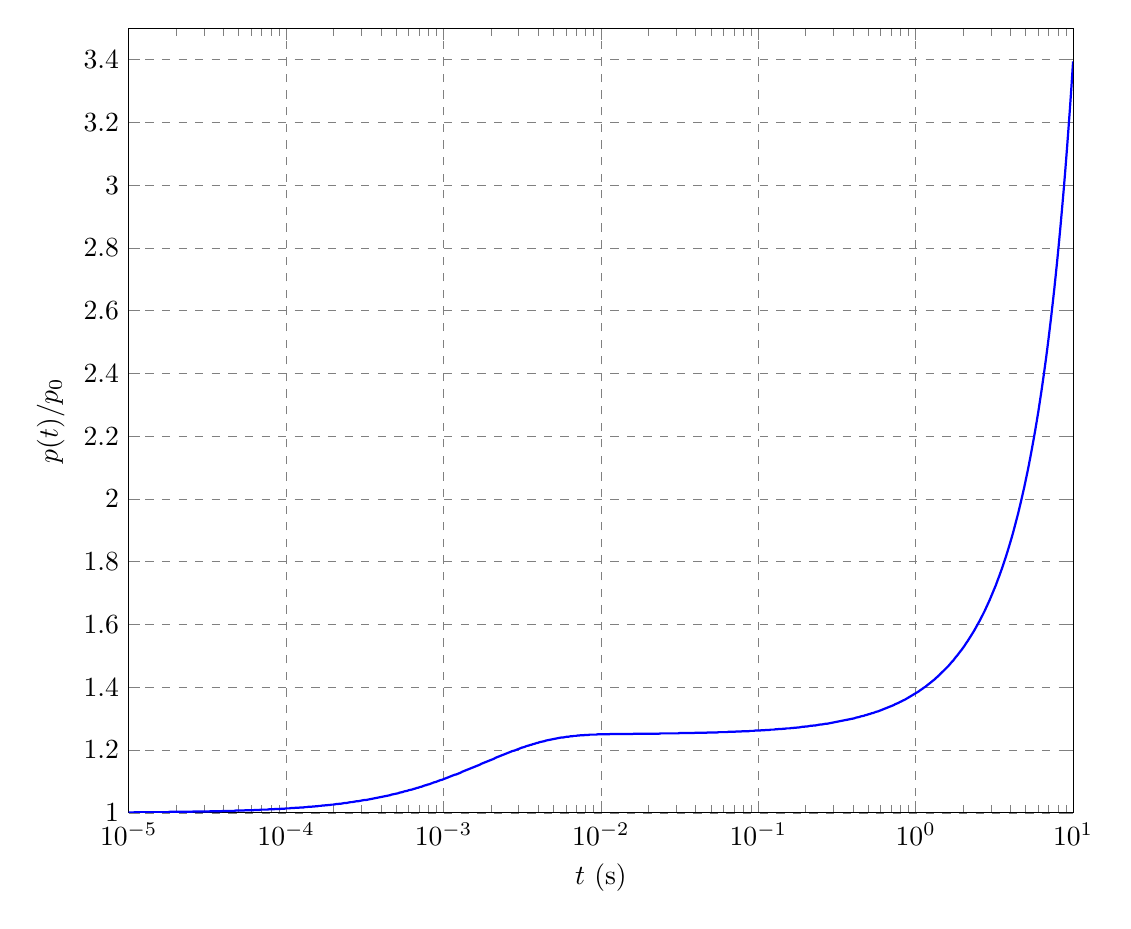
\begin{tikzpicture} \begin{axis}
[scale=1.75, xmode=log,
 xmin=1e-5, xmax=10,
 ymin=1, ymax=3.5,
 grid=major, 
 major grid style={color=gray,line width=0.2pt, dashed},
 xlabel=$t$ (s),
 ylabel=$p(t)/p_0$,
]

\addplot[line width=0.8pt, color=blue] coordinates {
( 1.000e-05, 1.001e+00 ) ( 1.023e-05, 1.001e+00 ) ( 1.047e-05, 1.001e+00 ) ( 1.072e-05, 1.001e+00 ) ( 1.096e-05, 1.002e+00 ) ( 1.122e-05, 1.002e+00 ) ( 1.148e-05, 1.002e+00 ) ( 1.175e-05, 1.002e+00 ) ( 1.202e-05, 1.002e+00 ) ( 1.230e-05, 1.002e+00 ) ( 1.259e-05, 1.002e+00 ) ( 1.288e-05, 1.002e+00 ) ( 1.318e-05, 1.002e+00 ) ( 1.349e-05, 1.002e+00 ) ( 1.380e-05, 1.002e+00 ) ( 1.413e-05, 1.002e+00 ) ( 1.445e-05, 1.002e+00 ) ( 1.479e-05, 1.002e+00 ) ( 1.514e-05, 1.002e+00 ) ( 1.549e-05, 1.002e+00 ) ( 1.585e-05, 1.002e+00 ) ( 1.622e-05, 1.002e+00 ) ( 1.660e-05, 1.002e+00 ) ( 1.698e-05, 1.002e+00 ) ( 1.738e-05, 1.002e+00 ) ( 1.778e-05, 1.002e+00 ) ( 1.820e-05, 1.003e+00 ) ( 1.862e-05, 1.003e+00 ) ( 1.905e-05, 1.003e+00 ) ( 1.950e-05, 1.003e+00 ) ( 1.995e-05, 1.003e+00 ) ( 2.042e-05, 1.003e+00 ) ( 2.089e-05, 1.003e+00 ) ( 2.138e-05, 1.003e+00 ) ( 2.188e-05, 1.003e+00 ) ( 2.239e-05, 1.003e+00 ) ( 2.291e-05, 1.003e+00 ) ( 2.344e-05, 1.003e+00 ) ( 2.399e-05, 1.003e+00 ) ( 2.455e-05, 1.003e+00 ) ( 2.512e-05, 1.003e+00 ) ( 2.570e-05, 1.004e+00 ) ( 2.630e-05, 1.004e+00 ) ( 2.692e-05, 1.004e+00 ) ( 2.754e-05, 1.004e+00 ) ( 2.818e-05, 1.004e+00 ) ( 2.884e-05, 1.004e+00 ) ( 2.951e-05, 1.004e+00 ) ( 3.020e-05, 1.004e+00 ) ( 3.090e-05, 1.004e+00 ) ( 3.162e-05, 1.004e+00 ) ( 3.236e-05, 1.004e+00 ) ( 3.311e-05, 1.005e+00 ) ( 3.388e-05, 1.005e+00 ) ( 3.467e-05, 1.005e+00 ) ( 3.548e-05, 1.005e+00 ) ( 3.631e-05, 1.005e+00 ) ( 3.715e-05, 1.005e+00 ) ( 3.802e-05, 1.005e+00 ) ( 3.890e-05, 1.005e+00 ) ( 3.981e-05, 1.006e+00 ) ( 4.074e-05, 1.006e+00 ) ( 4.169e-05, 1.006e+00 ) ( 4.266e-05, 1.006e+00 ) ( 4.365e-05, 1.006e+00 ) ( 4.467e-05, 1.006e+00 ) ( 4.571e-05, 1.006e+00 ) ( 4.677e-05, 1.006e+00 ) ( 4.786e-05, 1.007e+00 ) ( 4.898e-05, 1.007e+00 ) ( 5.012e-05, 1.007e+00 ) ( 5.129e-05, 1.007e+00 ) ( 5.248e-05, 1.007e+00 ) ( 5.370e-05, 1.007e+00 ) ( 5.495e-05, 1.008e+00 ) ( 5.623e-05, 1.008e+00 ) ( 5.754e-05, 1.008e+00 ) ( 5.888e-05, 1.008e+00 ) ( 6.026e-05, 1.008e+00 ) ( 6.166e-05, 1.008e+00 ) ( 6.310e-05, 1.009e+00 ) ( 6.457e-05, 1.009e+00 ) ( 6.607e-05, 1.009e+00 ) ( 6.761e-05, 1.009e+00 ) ( 6.918e-05, 1.010e+00 ) ( 7.079e-05, 1.010e+00 ) ( 7.244e-05, 1.010e+00 ) ( 7.413e-05, 1.010e+00 ) ( 7.586e-05, 1.010e+00 ) ( 7.762e-05, 1.011e+00 ) ( 7.943e-05, 1.011e+00 ) ( 8.128e-05, 1.011e+00 ) ( 8.318e-05, 1.011e+00 ) ( 8.511e-05, 1.012e+00 ) ( 8.710e-05, 1.012e+00 ) ( 8.913e-05, 1.012e+00 ) ( 9.120e-05, 1.012e+00 ) ( 9.333e-05, 1.013e+00 ) ( 9.550e-05, 1.013e+00 ) ( 9.772e-05, 1.013e+00 ) ( 1.000e-04, 1.014e+00 ) ( 1.023e-04, 1.014e+00 ) ( 1.047e-04, 1.014e+00 ) ( 1.072e-04, 1.015e+00 ) ( 1.096e-04, 1.015e+00 ) ( 1.122e-04, 1.015e+00 ) ( 1.148e-04, 1.016e+00 ) ( 1.175e-04, 1.016e+00 ) ( 1.202e-04, 1.016e+00 ) ( 1.230e-04, 1.017e+00 ) ( 1.259e-04, 1.017e+00 ) ( 1.288e-04, 1.017e+00 ) ( 1.318e-04, 1.018e+00 ) ( 1.349e-04, 1.018e+00 ) ( 1.380e-04, 1.019e+00 ) ( 1.413e-04, 1.019e+00 ) ( 1.445e-04, 1.019e+00 ) ( 1.479e-04, 1.020e+00 ) ( 1.514e-04, 1.020e+00 ) ( 1.549e-04, 1.021e+00 ) ( 1.585e-04, 1.021e+00 ) ( 1.622e-04, 1.022e+00 ) ( 1.660e-04, 1.022e+00 ) ( 1.698e-04, 1.023e+00 ) ( 1.738e-04, 1.023e+00 ) ( 1.778e-04, 1.024e+00 ) ( 1.820e-04, 1.024e+00 ) ( 1.862e-04, 1.025e+00 ) ( 1.905e-04, 1.025e+00 ) ( 1.950e-04, 1.026e+00 ) ( 1.995e-04, 1.026e+00 ) ( 2.042e-04, 1.027e+00 ) ( 2.089e-04, 1.028e+00 ) ( 2.138e-04, 1.028e+00 ) ( 2.188e-04, 1.029e+00 ) ( 2.239e-04, 1.029e+00 ) ( 2.291e-04, 1.030e+00 ) ( 2.344e-04, 1.031e+00 ) ( 2.399e-04, 1.031e+00 ) ( 2.455e-04, 1.032e+00 ) ( 2.512e-04, 1.033e+00 ) ( 2.570e-04, 1.034e+00 ) ( 2.630e-04, 1.034e+00 ) ( 2.692e-04, 1.035e+00 ) ( 2.754e-04, 1.036e+00 ) ( 2.818e-04, 1.037e+00 ) ( 2.884e-04, 1.037e+00 ) ( 2.951e-04, 1.038e+00 ) ( 3.020e-04, 1.039e+00 ) ( 3.090e-04, 1.040e+00 ) ( 3.162e-04, 1.041e+00 ) ( 3.236e-04, 1.041e+00 ) ( 3.311e-04, 1.042e+00 ) ( 3.388e-04, 1.043e+00 ) ( 3.467e-04, 1.044e+00 ) ( 3.548e-04, 1.045e+00 ) ( 3.631e-04, 1.046e+00 ) ( 3.715e-04, 1.047e+00 ) ( 3.802e-04, 1.048e+00 ) ( 3.890e-04, 1.049e+00 ) ( 3.981e-04, 1.050e+00 ) ( 4.074e-04, 1.051e+00 ) ( 4.169e-04, 1.052e+00 ) ( 4.266e-04, 1.053e+00 ) ( 4.365e-04, 1.054e+00 ) ( 4.467e-04, 1.055e+00 ) ( 4.571e-04, 1.056e+00 ) ( 4.677e-04, 1.058e+00 ) ( 4.786e-04, 1.059e+00 ) ( 4.898e-04, 1.060e+00 ) ( 5.012e-04, 1.061e+00 ) ( 5.129e-04, 1.062e+00 ) ( 5.248e-04, 1.064e+00 ) ( 5.370e-04, 1.065e+00 ) ( 5.495e-04, 1.066e+00 ) ( 5.623e-04, 1.068e+00 ) ( 5.754e-04, 1.069e+00 ) ( 5.888e-04, 1.070e+00 ) ( 6.026e-04, 1.072e+00 ) ( 6.166e-04, 1.073e+00 ) ( 6.310e-04, 1.074e+00 ) ( 6.457e-04, 1.076e+00 ) ( 6.607e-04, 1.077e+00 ) ( 6.761e-04, 1.079e+00 ) ( 6.918e-04, 1.080e+00 ) ( 7.079e-04, 1.082e+00 ) ( 7.244e-04, 1.083e+00 ) ( 7.413e-04, 1.085e+00 ) ( 7.586e-04, 1.087e+00 ) ( 7.762e-04, 1.088e+00 ) ( 7.943e-04, 1.090e+00 ) ( 8.128e-04, 1.091e+00 ) ( 8.318e-04, 1.093e+00 ) ( 8.511e-04, 1.095e+00 ) ( 8.710e-04, 1.097e+00 ) ( 8.913e-04, 1.098e+00 ) ( 9.120e-04, 1.100e+00 ) ( 9.333e-04, 1.102e+00 ) ( 9.550e-04, 1.104e+00 ) ( 9.772e-04, 1.105e+00 ) ( 1.000e-03, 1.107e+00 ) ( 1.023e-03, 1.109e+00 ) ( 1.047e-03, 1.111e+00 ) ( 1.072e-03, 1.113e+00 ) ( 1.096e-03, 1.115e+00 ) ( 1.122e-03, 1.117e+00 ) ( 1.148e-03, 1.119e+00 ) ( 1.175e-03, 1.121e+00 ) ( 1.202e-03, 1.122e+00 ) ( 1.230e-03, 1.124e+00 ) ( 1.259e-03, 1.126e+00 ) ( 1.288e-03, 1.128e+00 ) ( 1.318e-03, 1.131e+00 ) ( 1.349e-03, 1.133e+00 ) ( 1.380e-03, 1.135e+00 ) ( 1.413e-03, 1.137e+00 ) ( 1.445e-03, 1.139e+00 ) ( 1.479e-03, 1.141e+00 ) ( 1.514e-03, 1.143e+00 ) ( 1.549e-03, 1.145e+00 ) ( 1.585e-03, 1.147e+00 ) ( 1.622e-03, 1.149e+00 ) ( 1.660e-03, 1.151e+00 ) ( 1.698e-03, 1.153e+00 ) ( 1.738e-03, 1.156e+00 ) ( 1.778e-03, 1.158e+00 ) ( 1.820e-03, 1.160e+00 ) ( 1.862e-03, 1.162e+00 ) ( 1.905e-03, 1.164e+00 ) ( 1.950e-03, 1.166e+00 ) ( 1.995e-03, 1.168e+00 ) ( 2.042e-03, 1.170e+00 ) ( 2.089e-03, 1.172e+00 ) ( 2.138e-03, 1.175e+00 ) ( 2.188e-03, 1.177e+00 ) ( 2.239e-03, 1.179e+00 ) ( 2.291e-03, 1.181e+00 ) ( 2.344e-03, 1.183e+00 ) ( 2.399e-03, 1.185e+00 ) ( 2.455e-03, 1.187e+00 ) ( 2.512e-03, 1.189e+00 ) ( 2.570e-03, 1.191e+00 ) ( 2.630e-03, 1.193e+00 ) ( 2.692e-03, 1.195e+00 ) ( 2.754e-03, 1.197e+00 ) ( 2.818e-03, 1.198e+00 ) ( 2.884e-03, 1.200e+00 ) ( 2.951e-03, 1.202e+00 ) ( 3.020e-03, 1.204e+00 ) ( 3.090e-03, 1.206e+00 ) ( 3.162e-03, 1.208e+00 ) ( 3.236e-03, 1.209e+00 ) ( 3.311e-03, 1.211e+00 ) ( 3.388e-03, 1.213e+00 ) ( 3.467e-03, 1.214e+00 ) ( 3.548e-03, 1.216e+00 ) ( 3.631e-03, 1.217e+00 ) ( 3.715e-03, 1.219e+00 ) ( 3.802e-03, 1.220e+00 ) ( 3.890e-03, 1.222e+00 ) ( 3.981e-03, 1.223e+00 ) ( 4.074e-03, 1.225e+00 ) ( 4.169e-03, 1.226e+00 ) ( 4.266e-03, 1.227e+00 ) ( 4.365e-03, 1.228e+00 ) ( 4.467e-03, 1.230e+00 ) ( 4.571e-03, 1.231e+00 ) ( 4.677e-03, 1.232e+00 ) ( 4.786e-03, 1.233e+00 ) ( 4.898e-03, 1.234e+00 ) ( 5.012e-03, 1.235e+00 ) ( 5.129e-03, 1.236e+00 ) ( 5.248e-03, 1.237e+00 ) ( 5.370e-03, 1.238e+00 ) ( 5.495e-03, 1.239e+00 ) ( 5.623e-03, 1.240e+00 ) ( 5.754e-03, 1.240e+00 ) ( 5.888e-03, 1.241e+00 ) ( 6.026e-03, 1.242e+00 ) ( 6.166e-03, 1.242e+00 ) ( 6.310e-03, 1.243e+00 ) ( 6.457e-03, 1.244e+00 ) ( 6.607e-03, 1.244e+00 ) ( 6.761e-03, 1.245e+00 ) ( 6.918e-03, 1.245e+00 ) ( 7.079e-03, 1.246e+00 ) ( 7.244e-03, 1.246e+00 ) ( 7.413e-03, 1.247e+00 ) ( 7.586e-03, 1.247e+00 ) ( 7.762e-03, 1.247e+00 ) ( 7.943e-03, 1.248e+00 ) ( 8.128e-03, 1.248e+00 ) ( 8.318e-03, 1.248e+00 ) ( 8.511e-03, 1.249e+00 ) ( 8.710e-03, 1.249e+00 ) ( 8.913e-03, 1.249e+00 ) ( 9.120e-03, 1.249e+00 ) ( 9.333e-03, 1.249e+00 ) ( 9.550e-03, 1.250e+00 ) ( 9.772e-03, 1.250e+00 ) ( 1.000e-02, 1.250e+00 ) ( 1.023e-02, 1.250e+00 ) ( 1.047e-02, 1.250e+00 ) ( 1.072e-02, 1.250e+00 ) ( 1.096e-02, 1.250e+00 ) ( 1.122e-02, 1.250e+00 ) ( 1.148e-02, 1.251e+00 ) ( 1.175e-02, 1.251e+00 ) ( 1.202e-02, 1.251e+00 ) ( 1.230e-02, 1.251e+00 ) ( 1.259e-02, 1.251e+00 ) ( 1.288e-02, 1.251e+00 ) ( 1.318e-02, 1.251e+00 ) ( 1.349e-02, 1.251e+00 ) ( 1.380e-02, 1.251e+00 ) ( 1.413e-02, 1.251e+00 ) ( 1.445e-02, 1.251e+00 ) ( 1.479e-02, 1.251e+00 ) ( 1.514e-02, 1.251e+00 ) ( 1.549e-02, 1.251e+00 ) ( 1.585e-02, 1.251e+00 ) ( 1.622e-02, 1.252e+00 ) ( 1.660e-02, 1.252e+00 ) ( 1.698e-02, 1.252e+00 ) ( 1.738e-02, 1.252e+00 ) ( 1.778e-02, 1.252e+00 ) ( 1.820e-02, 1.252e+00 ) ( 1.862e-02, 1.252e+00 ) ( 1.905e-02, 1.252e+00 ) ( 1.950e-02, 1.252e+00 ) ( 1.995e-02, 1.252e+00 ) ( 2.042e-02, 1.252e+00 ) ( 2.089e-02, 1.252e+00 ) ( 2.138e-02, 1.252e+00 ) ( 2.188e-02, 1.252e+00 ) ( 2.239e-02, 1.252e+00 ) ( 2.291e-02, 1.252e+00 ) ( 2.344e-02, 1.252e+00 ) ( 2.399e-02, 1.253e+00 ) ( 2.455e-02, 1.253e+00 ) ( 2.512e-02, 1.253e+00 ) ( 2.570e-02, 1.253e+00 ) ( 2.630e-02, 1.253e+00 ) ( 2.692e-02, 1.253e+00 ) ( 2.754e-02, 1.253e+00 ) ( 2.818e-02, 1.253e+00 ) ( 2.884e-02, 1.253e+00 ) ( 2.951e-02, 1.253e+00 ) ( 3.020e-02, 1.253e+00 ) ( 3.090e-02, 1.253e+00 ) ( 3.162e-02, 1.254e+00 ) ( 3.236e-02, 1.254e+00 ) ( 3.311e-02, 1.254e+00 ) ( 3.388e-02, 1.254e+00 ) ( 3.467e-02, 1.254e+00 ) ( 3.548e-02, 1.254e+00 ) ( 3.631e-02, 1.254e+00 ) ( 3.715e-02, 1.254e+00 ) ( 3.802e-02, 1.254e+00 ) ( 3.890e-02, 1.254e+00 ) ( 3.981e-02, 1.255e+00 ) ( 4.074e-02, 1.255e+00 ) ( 4.169e-02, 1.255e+00 ) ( 4.266e-02, 1.255e+00 ) ( 4.365e-02, 1.255e+00 ) ( 4.467e-02, 1.255e+00 ) ( 4.571e-02, 1.255e+00 ) ( 4.677e-02, 1.255e+00 ) ( 4.786e-02, 1.256e+00 ) ( 4.898e-02, 1.256e+00 ) ( 5.012e-02, 1.256e+00 ) ( 5.129e-02, 1.256e+00 ) ( 5.248e-02, 1.256e+00 ) ( 5.370e-02, 1.256e+00 ) ( 5.495e-02, 1.256e+00 ) ( 5.623e-02, 1.257e+00 ) ( 5.754e-02, 1.257e+00 ) ( 5.888e-02, 1.257e+00 ) ( 6.026e-02, 1.257e+00 ) ( 6.166e-02, 1.257e+00 ) ( 6.310e-02, 1.257e+00 ) ( 6.457e-02, 1.258e+00 ) ( 6.607e-02, 1.258e+00 ) ( 6.761e-02, 1.258e+00 ) ( 6.918e-02, 1.258e+00 ) ( 7.079e-02, 1.258e+00 ) ( 7.244e-02, 1.259e+00 ) ( 7.413e-02, 1.259e+00 ) ( 7.586e-02, 1.259e+00 ) ( 7.762e-02, 1.259e+00 ) ( 7.943e-02, 1.260e+00 ) ( 8.128e-02, 1.260e+00 ) ( 8.318e-02, 1.260e+00 ) ( 8.511e-02, 1.260e+00 ) ( 8.710e-02, 1.260e+00 ) ( 8.913e-02, 1.261e+00 ) ( 9.120e-02, 1.261e+00 ) ( 9.333e-02, 1.261e+00 ) ( 9.550e-02, 1.262e+00 ) ( 9.772e-02, 1.262e+00 ) ( 1.000e-01, 1.262e+00 ) ( 1.023e-01, 1.262e+00 ) ( 1.047e-01, 1.263e+00 ) ( 1.072e-01, 1.263e+00 ) ( 1.096e-01, 1.263e+00 ) ( 1.122e-01, 1.264e+00 ) ( 1.148e-01, 1.264e+00 ) ( 1.175e-01, 1.264e+00 ) ( 1.202e-01, 1.265e+00 ) ( 1.230e-01, 1.265e+00 ) ( 1.259e-01, 1.265e+00 ) ( 1.288e-01, 1.266e+00 ) ( 1.318e-01, 1.266e+00 ) ( 1.349e-01, 1.267e+00 ) ( 1.380e-01, 1.267e+00 ) ( 1.413e-01, 1.267e+00 ) ( 1.445e-01, 1.268e+00 ) ( 1.479e-01, 1.268e+00 ) ( 1.514e-01, 1.269e+00 ) ( 1.549e-01, 1.269e+00 ) ( 1.585e-01, 1.269e+00 ) ( 1.622e-01, 1.270e+00 ) ( 1.660e-01, 1.270e+00 ) ( 1.698e-01, 1.271e+00 ) ( 1.738e-01, 1.271e+00 ) ( 1.778e-01, 1.272e+00 ) ( 1.820e-01, 1.272e+00 ) ( 1.862e-01, 1.273e+00 ) ( 1.905e-01, 1.274e+00 ) ( 1.950e-01, 1.274e+00 ) ( 1.995e-01, 1.275e+00 ) ( 2.042e-01, 1.275e+00 ) ( 2.089e-01, 1.276e+00 ) ( 2.138e-01, 1.277e+00 ) ( 2.188e-01, 1.277e+00 ) ( 2.239e-01, 1.278e+00 ) ( 2.291e-01, 1.278e+00 ) ( 2.344e-01, 1.279e+00 ) ( 2.399e-01, 1.280e+00 ) ( 2.455e-01, 1.281e+00 ) ( 2.512e-01, 1.281e+00 ) ( 2.570e-01, 1.282e+00 ) ( 2.630e-01, 1.283e+00 ) ( 2.692e-01, 1.284e+00 ) ( 2.754e-01, 1.284e+00 ) ( 2.818e-01, 1.285e+00 ) ( 2.884e-01, 1.286e+00 ) ( 2.951e-01, 1.287e+00 ) ( 3.020e-01, 1.288e+00 ) ( 3.090e-01, 1.289e+00 ) ( 3.162e-01, 1.290e+00 ) ( 3.236e-01, 1.291e+00 ) ( 3.311e-01, 1.292e+00 ) ( 3.388e-01, 1.293e+00 ) ( 3.467e-01, 1.294e+00 ) ( 3.548e-01, 1.295e+00 ) ( 3.631e-01, 1.296e+00 ) ( 3.715e-01, 1.297e+00 ) ( 3.802e-01, 1.298e+00 ) ( 3.890e-01, 1.299e+00 ) ( 3.981e-01, 1.300e+00 ) ( 4.074e-01, 1.301e+00 ) ( 4.169e-01, 1.303e+00 ) ( 4.266e-01, 1.304e+00 ) ( 4.365e-01, 1.305e+00 ) ( 4.467e-01, 1.307e+00 ) ( 4.571e-01, 1.308e+00 ) ( 4.677e-01, 1.309e+00 ) ( 4.786e-01, 1.311e+00 ) ( 4.898e-01, 1.312e+00 ) ( 5.012e-01, 1.314e+00 ) ( 5.129e-01, 1.315e+00 ) ( 5.248e-01, 1.317e+00 ) ( 5.370e-01, 1.318e+00 ) ( 5.495e-01, 1.320e+00 ) ( 5.623e-01, 1.322e+00 ) ( 5.754e-01, 1.323e+00 ) ( 5.888e-01, 1.325e+00 ) ( 6.026e-01, 1.327e+00 ) ( 6.166e-01, 1.329e+00 ) ( 6.310e-01, 1.331e+00 ) ( 6.457e-01, 1.333e+00 ) ( 6.607e-01, 1.335e+00 ) ( 6.761e-01, 1.337e+00 ) ( 6.918e-01, 1.339e+00 ) ( 7.079e-01, 1.341e+00 ) ( 7.244e-01, 1.343e+00 ) ( 7.413e-01, 1.346e+00 ) ( 7.586e-01, 1.348e+00 ) ( 7.762e-01, 1.350e+00 ) ( 7.943e-01, 1.353e+00 ) ( 8.128e-01, 1.355e+00 ) ( 8.318e-01, 1.358e+00 ) ( 8.511e-01, 1.360e+00 ) ( 8.710e-01, 1.363e+00 ) ( 8.913e-01, 1.366e+00 ) ( 9.120e-01, 1.369e+00 ) ( 9.333e-01, 1.372e+00 ) ( 9.550e-01, 1.375e+00 ) ( 9.772e-01, 1.378e+00 ) ( 1.000e+00, 1.381e+00 ) ( 1.023e+00, 1.384e+00 ) ( 1.047e+00, 1.387e+00 ) ( 1.072e+00, 1.391e+00 ) ( 1.096e+00, 1.394e+00 ) ( 1.122e+00, 1.398e+00 ) ( 1.148e+00, 1.401e+00 ) ( 1.175e+00, 1.405e+00 ) ( 1.202e+00, 1.409e+00 ) ( 1.230e+00, 1.413e+00 ) ( 1.259e+00, 1.417e+00 ) ( 1.288e+00, 1.421e+00 ) ( 1.318e+00, 1.425e+00 ) ( 1.349e+00, 1.430e+00 ) ( 1.380e+00, 1.434e+00 ) ( 1.413e+00, 1.439e+00 ) ( 1.445e+00, 1.444e+00 ) ( 1.479e+00, 1.449e+00 ) ( 1.514e+00, 1.454e+00 ) ( 1.549e+00, 1.459e+00 ) ( 1.585e+00, 1.464e+00 ) ( 1.622e+00, 1.469e+00 ) ( 1.660e+00, 1.475e+00 ) ( 1.698e+00, 1.481e+00 ) ( 1.738e+00, 1.486e+00 ) ( 1.778e+00, 1.493e+00 ) ( 1.820e+00, 1.499e+00 ) ( 1.862e+00, 1.505e+00 ) ( 1.905e+00, 1.512e+00 ) ( 1.950e+00, 1.518e+00 ) ( 1.995e+00, 1.525e+00 ) ( 2.042e+00, 1.532e+00 ) ( 2.089e+00, 1.540e+00 ) ( 2.138e+00, 1.547e+00 ) ( 2.188e+00, 1.555e+00 ) ( 2.239e+00, 1.563e+00 ) ( 2.291e+00, 1.571e+00 ) ( 2.344e+00, 1.579e+00 ) ( 2.399e+00, 1.588e+00 ) ( 2.455e+00, 1.597e+00 ) ( 2.512e+00, 1.606e+00 ) ( 2.570e+00, 1.615e+00 ) ( 2.630e+00, 1.625e+00 ) ( 2.692e+00, 1.635e+00 ) ( 2.754e+00, 1.645e+00 ) ( 2.818e+00, 1.656e+00 ) ( 2.884e+00, 1.667e+00 ) ( 2.951e+00, 1.678e+00 ) ( 3.020e+00, 1.690e+00 ) ( 3.090e+00, 1.702e+00 ) ( 3.162e+00, 1.714e+00 ) ( 3.236e+00, 1.726e+00 ) ( 3.311e+00, 1.740e+00 ) ( 3.388e+00, 1.753e+00 ) ( 3.467e+00, 1.767e+00 ) ( 3.548e+00, 1.781e+00 ) ( 3.631e+00, 1.796e+00 ) ( 3.715e+00, 1.811e+00 ) ( 3.802e+00, 1.827e+00 ) ( 3.890e+00, 1.843e+00 ) ( 3.981e+00, 1.860e+00 ) ( 4.074e+00, 1.877e+00 ) ( 4.169e+00, 1.895e+00 ) ( 4.266e+00, 1.914e+00 ) ( 4.365e+00, 1.933e+00 ) ( 4.467e+00, 1.952e+00 ) ( 4.571e+00, 1.973e+00 ) ( 4.677e+00, 1.994e+00 ) ( 4.786e+00, 2.016e+00 ) ( 4.898e+00, 2.038e+00 ) ( 5.012e+00, 2.062e+00 ) ( 5.129e+00, 2.086e+00 ) ( 5.248e+00, 2.111e+00 ) ( 5.370e+00, 2.137e+00 ) ( 5.495e+00, 2.164e+00 ) ( 5.623e+00, 2.192e+00 ) ( 5.754e+00, 2.220e+00 ) ( 5.888e+00, 2.250e+00 ) ( 6.026e+00, 2.281e+00 ) ( 6.166e+00, 2.314e+00 ) ( 6.310e+00, 2.347e+00 ) ( 6.457e+00, 2.382e+00 ) ( 6.607e+00, 2.418e+00 ) ( 6.761e+00, 2.455e+00 ) ( 6.918e+00, 2.494e+00 ) ( 7.079e+00, 2.535e+00 ) ( 7.244e+00, 2.577e+00 ) ( 7.413e+00, 2.621e+00 ) ( 7.586e+00, 2.666e+00 ) ( 7.762e+00, 2.714e+00 ) ( 7.943e+00, 2.763e+00 ) ( 8.128e+00, 2.815e+00 ) ( 8.318e+00, 2.869e+00 ) ( 8.511e+00, 2.925e+00 ) ( 8.710e+00, 2.983e+00 ) ( 8.913e+00, 3.044e+00 ) ( 9.120e+00, 3.108e+00 ) ( 9.333e+00, 3.175e+00 ) ( 9.550e+00, 3.244e+00 ) ( 9.772e+00, 3.317e+00 ) ( 1.000e+01, 3.394e+00 ) 
};

%\legend{Fuel,Moderator}
\end{axis}
\end{tikzpicture}
\caption{Point kinetics model of a positive reactivity insertion in a critical reactor using one delayed neutron precursor group.}
 \label{Fig:kinetics_pointKineticsCriticalReactor_1group}
\end{center}
\end{figure}

An illustration of the point kinetics solution is depicted in Fig.~\ref{Fig:kinetics_pointKineticsCriticalReactor_1group} on semi-logarithmic scale in the time dimension. Here we use 
\begin{align}
  \beta = 0.007, \ \Lambda = 10^{-5} \text{ s}, \ \lambda = 0.4 \text{ s$^{-1}$, and } \rho_1 = 0.2\text{\textcent}. \nonumber
\end{align}
As expected we observe the power level rise twice. One on the short time scale, where an equilibrium level is reached within about $10^{-2}$ seconds of the start of the insertion. This again is for the immediate equilibration of prompt neutrons. Between 0.1 and 1 seconds, the power level begins to increase exponentially again as delayed neutron precursors buildup. This exponential rise continues indefinitely (at least until feedback occurs). 

Note that while the trends are correct and representative of what would occur in an actual reactor, the use of only a single delayed precursor group leads to the power increasing much faster than would occur in reality during late times. To get this correct, we would need to use at the six delayed precursor groups. The difference is the power would still rise smoothly in late times (i.e., it would not level off for some time interval) but would gradually blend together as the different precursor groups build in. 

\subsection{Inhour Equation and Asymptotic Inverse Period}

One question we would like to answer is finding the amount of reactivity $\rho$ we need to insert into a reactor to achieve a particular exponential rate of power rise (or fall) after any initial effects have subsided. This relationship is called the \emph{inhour equation}. (Supposedly, the naming is motivated by finding the tiny amount of reactivity that would be inserted into a critical such that the reactor such that the power would multiply by a factor of $e$ after one hour.) This inhour equation is also very useful in analyzing the asymptotic behavior from various reactivity insertions.

We return to the simple kinetics equation
\begin{align}
  \frac{dp}{dt} = \alpha(t) p(t),
\end{align}
where $\alpha(t)$ is a time-dependent inverse period of the reactor (including both prompt and delayed neutrons, in contrast to $\alpha_p$), which considers all the various effects from prompt rise to buildup of delayed neutron precursors and potentially even feedback effects. If we somehow know $\alpha(t)$, we could calculate the power by simply solving the differential equation:
\begin{align}
  p(t) = p_0 \exp\left[ \int_0^t \alpha(t') dt' \right] .
\end{align}

Of course, we do not normally know $\alpha(t)$, but we can infer something about it if we neglect feedback. Based on the previous results, we noticed that eventually a single exponential term dominates. This motivates separating $\alpha(t)$ into a constant asymptotic and time-dependent ephemeral parts:
\begin{align}
  \alpha(t) = \alpha + \delta\alpha(t) ,
\end{align}
where the ephemeral part $\delta\alpha(\infty) = 0$. Plugging this into the exponential solution and separating out the exponential of a sum as the product of exponentials, we get for late times
\begin{align}
  p(t) = p_0 \exp \left[ \int_0^t \delta\alpha(t') dt' \right] \exp \left[ \int_0^t \alpha dt' \right] = p_\infty e^{\alpha t } , \quad t \gg 0 . \label{Eq:kinetics_pointKineticsInhour_powerAsymptotic}
\end{align}
Here $p_\infty$ includes the initial parts of the transients and converges to a constant value as $t$ becomes large.

Of course, delayed neutrons are an important part of many reactor transients, so we should describe them as well. Mathematically, we expect the precursor concentrations to follow the same general functional behavior as the power, but be shifted in time. The reduced precursor density can be written in terms of a convolution integral involving the power history of the reactor. This is, for the $i$th precursor group,
\begin{align}
  \zeta_i(t) = \beta_i \int_{-\infty}^t p(t') e^{-\lambda_i ( t - t' ) } dt' .
\end{align}
This convolution integral produces delayed neutron precursors at some time $t'$ and decays them exponentially from their birth up to time $t$. Currently, we are most interested in the asymptotic behavior, so we can insert Eq.~\eqref{Eq:kinetics_pointKineticsInhour_powerAsymptotic} into this and carry out the integral to obtain,
\begin{align}
  \zeta_{i,\infty}(t) 
  &= \beta_i \int_{-\infty}^t p_\infty \exp \left[ \alpha t' - \lambda_i ( t - t' ) \right] dt'
  = \frac{ \beta_i }{ \alpha + \lambda_i } p_\infty e^{\alpha t} , \quad t \gg 0. \label{Eq:kinetics_asymptoticReducedPrecursorConcentration}
\end{align}
We can then compute the total source of delayed neutrons by multiplying this result for each precursor group by the respective decay constant $\lambda_i$ and adding them up:
\begin{align}
  s_d(t) = \sum_i \frac{ \beta_i \lambda_i }{ \alpha + \lambda_i }  p_\infty e^{\alpha t} , \quad t \gg 0. \label{Eq:kinetics_asymptoticDelayedNeutronSource}
\end{align}

We can now return to the point kinetics equation for the reactor power, but apply it to late times. The time derivative on the left-hand side becomes
\begin{subequations}
\begin{align}
  \frac{dp}{dt} = \alpha(t) p(t) \rightarrow \alpha p_\infty e^{\alpha t} , \quad t \gg 0.
\end{align}
The right-hand side of the point kinetics equation for late times in terms of the delayed source $s_d$ is then
\begin{align}
  \frac{ \rho - \beta }{ \Lambda } p(t) + s_d(t) = \frac{ \rho - \beta }{ \Lambda } p_\infty e^{\alpha t}  +   \frac{1}{\Lambda} \sum_i \frac{ \beta_i \lambda_i }{ \alpha + \lambda_i } p_\infty e^{\alpha t} .
\end{align}
\end{subequations}
Equating the left- and right-hand sides of the equation and cancelling out a common factor of $p_\infty e^{\alpha t}$ gives
\begin{align}
  \alpha = \frac{ \rho - \beta }{ \Lambda } +  \frac{1}{\Lambda} \sum_i \frac{ \beta_i \lambda_i }{ \alpha + \lambda_i } ,
\end{align}
which we can then solve of the reactivity $\rho$ to arrive at
\begin{align}
  \rho = \alpha \Lambda + \beta - \sum_i \frac{ \beta_i \lambda_i }{ \alpha + \lambda_i } . \label{Eq:kinetics_inhourEquation_initialForm}
\end{align}
We then expand out $\beta$ as the sum over precursor groups and combine terms:
\begin{align}
  \rho 
  &= \alpha \Lambda + \sum_i \beta_i - \sum_i \frac{ \beta_i \lambda_i }{ \alpha + \lambda_i } \nonumber \\
  &= \alpha \Lambda + \sum_i \left[ \beta_i - \frac{ \beta_i \lambda_i }{ \alpha + \lambda_i } \right] \nonumber \\
  &= \alpha \Lambda + \sum_i \left[ \frac{\beta_i (\alpha + \lambda_i)}{ \alpha + \lambda_i }  - \frac{ \beta_i \lambda_i }{ \alpha + \lambda_i } \right] , \nonumber 
\end{align}
and after cancelling the like $\lambda_i \beta_i$ term in the numerator within the summation we arrive at the conventional form of the inhour equation:
\begin{align}
  \rho = \alpha \Lambda + \sum_i \frac{ \beta_i \alpha }{ \alpha + \lambda_i } . \label{Eq:kinetics_inhourEquation}
\end{align}

Using this equation can then define the unit of reactivity of an inhour, corresponding to $\alpha = 1/3600$~s$^{-1}$. Inserting representative delayed neutron data, we get that
\begin{align}
  1 \text{ inhour} \approx 0.0035 \beta = 0.35\text{\textcent} . \nonumber
\end{align}
Again, this is a very small amount of reactivity and usually encountered in the context of small operational adjustments or particular experiments.

Now that we have the inhour equation we can explore the limiting cases for positive reactivity insertions and therefore values of $\alpha$. We can break these limiting cases into three types:
\begin{enumerate}
  \item Prompt transients (extremely large $\alpha$) where delayed neutrons can be completely neglected;
  \item rapid transients (large $\alpha$) where the decay of delayed neutrons produced during the transient can be neglected;
  \item very slow transients (very small $\alpha$).
\end{enumerate}

Prompt transients occur over such a fast timescale that $\alpha$ is so large that the third term in Eq.~\eqref{Eq:kinetics_inhourEquation_initialForm} is insignificant because the $\lambda_i$ are so small. This gives the result that
\begin{align}
  \rho = \alpha \Lambda + \beta.
\end{align}
Solving for $\alpha$ in this limit gives us the interpretation of $(\rho - \beta)/\Lambda$ as the inverse prompt period.

For rapid transients, we keep the third term in equation Eq.~\eqref{Eq:kinetics_inhourEquation_initialForm} but write the denominator as $\alpha + \lambda_i \approx \alpha$. This gives
\begin{align}
  \rho = \alpha \Lambda + \beta - \frac{1}{\alpha} \sum_i \beta_i \lambda_i .
\end{align}
The sum of the delayed precursor group fractions times the decay constants can be used to form an averaged decay constant,
\begin{align}
  \overline{\lambda} = \dfrac{ \displaystyle\sum_i \beta_i \lambda_i }{ \displaystyle\sum_i \beta_i } = \frac{1}{\beta} \displaystyle\sum_i \beta_i \lambda_i ,
\end{align}
giving
\begin{align}
  \rho = \alpha \Lambda + \beta \left( 1 - \frac{\overline{\lambda}}{\alpha} \right) .
\end{align}
This shows that for rapid transients, we can get away with using a single average precursor group. (Again, six groups are needed to get long time behavior on slower transients.) 

Additionally, we can consider the asymptotic delayed neutron source from Eq.~\eqref{Eq:kinetics_asymptoticDelayedNeutronSource} making the same approximation, $\alpha + \lambda_i \approx \alpha$, as before. Making this approximation and writing the result in terms of the integral over the power history, we see that
\begin{align}
  s_d(t) \approx \sum_i \frac{ \beta_i \lambda_i }{ \alpha }  p_\infty e^{\alpha t} = \beta \overline{\lambda} p_\infty \int_{-\infty}^t e^{\alpha t'} dt' ,
\end{align}
and comparing with Eq.~\eqref{Eq:kinetics_asymptoticReducedPrecursorConcentration}, we note that the integral excludes the decay term from the precursors. This result shows that while over the rapid transient, a significant inventory of delayed neutron precursors is produced, but these have not had enough time to substantively decay and produce delayed neutrons. This motivates treating the delayed neutron source as a constant.

Finally, for very slow transients, we have $\alpha \ll \lambda_k$ and we can take the inhour equation in Eq.~\eqref{Eq:kinetics_inhourEquation} and can write
\begin{align}
  \rho = \alpha \left( \Lambda +  \sum_i \frac{ \beta_i }{ \lambda_i } \right). 
\end{align}
Similar to the rapid transient case, we can define the mean of the inverses of the precursor decay constants as
\begin{align}
  \overline{\left(\frac{1}{\lambda}\right)} = \dfrac{ \displaystyle\sum_i \frac{\beta_i}{\lambda_i} }{ \displaystyle\sum_i \beta_i } = \frac{1}{\beta} \displaystyle\sum_i \frac{\beta_i}{\lambda_i} .
\end{align}
Applying this average gives
\begin{align}
  \rho = \alpha \left( \Lambda +  \beta  \overline{\left(\frac{1}{\lambda}\right)} \right). 
\end{align}
Interesting to note that $\Lambda$ is usually very small and since the $\lambda_i$ is also quite small the mean of its inverse is large. Therefore, the reactivity or prompt period $\alpha$ is primarily determined by the delayed neutrons and is largely insensitive to the prompt neutron lifetime. This makes sense since the reactivity insertion is tiny, so we expect the delayed neutrons, not the prompt behavior, to be driving the transient.

One other case that is important is a large negative reactivity insertion $\alpha \rightarrow -\infty$. If we inspect the inhour equation, we note that there are singularities in the denominators of the sum when $\alpha = -\lambda_i$. The largest value of these is $-\lambda_1$, corresponding to the longest-lived precursor. 

This has a very important implication: the slowest a reactor can shutdown is limited by the decay of the longest-lived delayed neutron precursor, $^{87}$Br. This makes sense because fission produces an inventory of these precursors that even if we shut off the fission reactions completely somehow, there is no practical way to remove those fission products. All we can then do is wait for them to decay. Therefore, when we shut down a reactor, we still have neutrons and fission occurring for minutes afterward, which creates additional heat generation (on top of the normal thermal load produced by the inventory of radioactive fission products) that must be removed to keep the fuel intact.

\section{Adjoint Function and Perturbations}

A common question an analyst needs to answer is how a change in a design input parameter impacts an output quantity of interest. Most common in reactor analysis the inputs are quantities such as moderator density, fuel temperature, fuel enrichment, control rod height, etc. and the output is typically the effective multiplication factor or reactivity. 

We are often interested in exploring the design space and finding a set of configurations that satisfy certain criteria, i.e., a critical reactor. Since the number of input parameters in a typical reactor is very large (each of the thousands of fuel pin or tens of assemblies could, in principle be different), we often perform what is called a sensitivity analysis. In this we determine what set of parameters are most influential in changing the reactivity. Additionally, we are also interested in quantifying uncertainties to ensure that the reactor design satisfies safety margins and perturbation theory can be used to predict the range of quantities that would be plausibly encountered given uncertainties in the input parameters such as nuclear cross sections or other design parameters that may be uncertainty because of, for example, manufacturing tolerances.

Additionally, the point kinetics equation we developed in the previous section are a bit ad hoc and based on the one-speed approximation, which is quite limiting given that we require at least two energy groups to get reasonable results for a thermal reactor. Extending these models to include energy dependence while retaining the their simplicity is not straightforward. To accomplish either of these goals, we need to use a mathematical object called the adjoint function, which we cover next.

\subsection{Adjoint Transport and Multigroup Diffusion Equation}

The adjoint function is the solution to a twin of sorts of the neutron transport equation. Here we derive the steady-state form of the adjoint transport equation, which is sufficient for the purposes of establishing perturbations and point kinetics. To do this, we take integrals of the neutron transport equation and through some manipulations we arrive at a new set of mathematical \emph{operators} that it turns out describes the transport process in reverse. For this reason the adjoint transport equation is sometimes called the backwards transport equation and the standard neutron transport equation is referred to as the forward transport equation. Given this, we can arrive at a physical interpretation of the adjoint function as the neutron importance toward a particular response. In the context of reactors, this importance measures the ability of a neutron to sustain the chain reaction in a multiplying system.

\subsubsection{Time-Dependent Transport Equation with Precursors}

We begin this derivation by introducing a bit of notation. Admittedly this, is a bit abstract at first, but as the derivation proceeds, it should hopefully become more concrete. First, we write down the time-dependent transport equation,
\begin{subequations} \label{Eq:kinetics_timeDependentTransportEquationsPrecursors}
\begin{align}
  &\frac{1}{v}\dho{\psi}{t} + \dir \cdot \nabla \psi(\pos,\dir,E,t) + \Sigma_t(\pos,E) \psi(\pos,\dir,E,t) \nonumber \\
  &= \int_0^\infty \int_{4\pi} \Sigma_s(\pos, \dir' \cdot \dir , E' \rightarrow E ) \psi(\pos,\dir',E',t) d\Omega' dE' \nonumber \\
  &+ \int_0^\infty \int_{4\pi} ( 1 - \beta ) \nu \Sigma_f(\pos,  E' ) \psi(\pos,\dir',E',t) d\Omega' dE' \nonumber \\
  &+ \sum_i \frac{\chi_i(E)}{4\pi} \lambda_i C_i(\pos,t) + Q(\pos,\dir,E) ,
\end{align}
and the precursor balance equations,
\begin{align}
  \dho{C_i}{t} + \lambda_i C_i(\pos,t) = \int_0^\infty \int_{4\pi} \beta_i \nu \Sigma_f(\pos,  E' ) \psi(\pos,\dir',E',t) d\Omega' dE' ,
\end{align}
in their full form. The initial and boundary conditions are
\begin{align}
  \psi(\pos,\dir,E,0) &= \psi_0(\pos, \dir, E ), \quad \pos \in \Gamma , \dir \in 4\pi, \\
  \psi(\pos,\dir,E,t) &= \psi^b(\pos,\dir,E,t), \quad \pos \in \partial \Gamma, \nhat \cdot \dir < 0, \\
  C_i(\pos,0) &= C_{i,0}(\pos) ), \quad \pos \in \Gamma .
\end{align}
\end{subequations}
Here again $\Gamma$ is some convex region and $\partial \Gamma$ denotes its boundary. The only significant simplifications to these equations are:
\begin{enumerate}
  \item The material properties (cross sections) are time independent;
  \item The internal source of neutrons is time independent;
  \item There is no internal source of delayed neutron precursors nor do they undergo motion.
\end{enumerate}

\subsubsection{Operators and Integration Shorthand}

Since writing this out multiple times is rather cumbersome and quite honestly obscures the main points, we introduce the following shorthand terms called operators. First, we bring the scattering term to the left-hand side and define the net migration operator:
\begin{subequations}
\begin{align}
  \mathcal{M} \psi = \dir \cdot \nabla \psi + \Sigma_t \psi - \int_0^\infty \int_{4\pi} \Sigma_s(\dir' \cdot \dir , E' \rightarrow E ) \psi(\dir',E') d\Omega' dE'.
\end{align}
where unnecessary functional dependences have been omitted for brevity. Next, we define the prompt fission operator as
\begin{align}
  \mathcal{F}_p \psi = \int_0^\infty \int_{4\pi} ( 1 - \beta ) \nu \Sigma_f( E' ) \psi(\dir',E') d\Omega' dE' .
\end{align}
We also define the production operator for delayed precursors in group $i$ as
\begin{align}
  \mathcal{B}_i \psi = \int_0^\infty \int_{4\pi} \beta_i \nu \Sigma_f( E' ) \psi(\dir',E') d\Omega' dE' .
\end{align}
Finally, for completeness, we define the \emph{total} fission operator in terms of the prompt and delayed components:
\begin{align}
  \mathcal{F} \psi = \mathcal{F}_p \psi + \sum_i \frac{\chi_i}{4\pi} \mathcal{B}_i \psi .
\end{align}
\end{subequations}

We can then write the neutron transport and precursor balance equations in shorthand as
\begin{subequations}
\begin{align}
  \frac{1}{v} \dho{\psi}{t} + \mathcal{M} \psi &= \mathcal{F}_p \psi + \sum_i \frac{\chi_i}{4\pi} \lambda_i C_i + Q , \\
  \dho{C_i}{t} + \lambda_i C_i &= \mathcal{B}_i \psi . 
\end{align}
We can easily arrive at the steady-state version by setting the time derivatives to zero and solving for the delayed neutron source. We get
\begin{align}
  \mathcal{M} \psi &= \mathcal{F} \psi + Q .
\end{align}
\end{subequations}

Next, we introduce another shorthand to denote integration over all positions in the reactor volume $\Gamma$, all directions, and all energies using angle brackets to denote an \emph{inner product}:
\begin{subequations}
\begin{align}
  \left< f, g \right> = \int_0^\infty \int_{4\pi} \int_\Gamma f(\pos,\dir,E,t) g(\pos,\dir,E,t) dV d\Omega dE , \label{Eq:kinetics_adjoint_volumeIntegralAngleBrackets}
\end{align}
where $f$ and $g$ are arbitrary functions. We also define the analogous surface integral over the boundary $\partial \Gamma$, all directions, and all energies using square brackets:
\begin{align}
  \left[ f, g \right] = \int_0^\infty \int_{4\pi} \int_{\partial \Gamma} (\nhat \cdot \dir ) f(\pos,\dir,E,t) g(\pos,\dir,E,t) dA d\Omega dE .  \label{Eq:kinetics_adjoint_surfaceIntegralSquareBrackets}
\end{align}
This is used to define the net current. Furthermore, we can break this up into incoming and outgoing directional components as
\begin{align}
  \left[ f, g \right]_- &= \int_0^\infty \int_{\nhat \cdot \dir < 0} \int_{\partial \Gamma}  (\nhat \cdot \dir )  f(\pos,\dir,E,t) g(\pos,\dir,E,t) dA d\Omega dE , \\
  \left[ f, g \right]_+ &= \int_0^\infty \int_{\nhat \cdot \dir > 0} \int_{\partial \Gamma}  |\nhat \cdot \dir | f(\pos,\dir,E,t) g(\pos,\dir,E,t) dA d\Omega dE ,
\end{align}
respectively to get the partial currents. This implies that the 
\begin{align}
  \left[ f, g \right] = \left[ f, g \right]_+ - \left[ f, g \right]_- ,
\end{align}
\end{subequations}
which follows from the definition that the net current is the outward partial current minus the inward partial current.

\subsubsection{Steady-State Adjoint Operators}

To arrive at the equation for the adjoint function, we take each of the terms in the steady-state transport equation and integrate them over all positions, energies, and directions. Using the transport equation in operator form, we can write
\begin{align}
  ( \mathcal{M} - \mathcal{F} ) f = Q , \label{Eq:kinetics_operatorFormAbstractSteadyStateTransport}
\end{align}
where $f$ is an arbitrary function of $(\pos,\dir,E)$ acted on by the physical operators of neutron transport.

We begin with the streaming or net leakage term. We take this term, multiply by some arbitrary function $g(\pos,\dir,E)$ and integrate over all position, direction, and energy. We obtain the expression
\begin{align}
  \int_0^\infty \int_{4\pi} \int_\Gamma g(\pos,\dir,E) ( \dir \cdot \nabla ) f(\pos,\dir,E) dV d\Omega dE . \nonumber
\end{align}
Now, we apply the product rule of gradients,
\begin{align}
  \nabla(fg) = f \nabla g + g \nabla f,
\end{align}
to write
\begin{align}
   &\int_0^\infty \int_{4\pi} \int_\Gamma g(\pos,\dir,E)  (\dir \cdot \nabla) f(\pos,\dir,E) dV d\Omega dE \nonumber \\
   &= \int_0^\infty \int_{4\pi} \int_\Gamma \dir \cdot \nabla \left[ f(\pos,\dir,E) g(\pos,\dir,E) \right] dV d\Omega dE \nonumber \\
   &- \int_0^\infty \int_{4\pi} \int_\Gamma f(\pos,\dir,E)  (\dir \cdot \nabla) g(\pos,\dir,E) dV d\Omega dE .
\end{align}

The term involving the gradient over the product of $f$ and $g$ can be converted into a surface integral using the divergence theorem:
\begin{align}
   &\int_0^\infty \int_{4\pi} \int_\Gamma \dir \cdot \nabla \left[ f(\pos,\dir,E) g(\pos,\dir,E) \right] dV d\Omega dE \nonumber \\
   &= \int_0^\infty \int_{4\pi} \int_{\partial \Gamma} ( \nhat \cdot \dir ) \nabla \left[ f(\pos,\dir,E) g(\pos,\dir,E) \right] dV d\Omega dE \nonumber \\
   &= [ f, g ].
\end{align}
Here we applied the shorthand for the surface integral using square brackets from Eq.~\eqref{Eq:kinetics_adjoint_surfaceIntegralSquareBrackets}.

Using the shorthand for the volume integral using angle braces from Eq.~\eqref{Eq:kinetics_adjoint_volumeIntegralAngleBrackets}, we can write this integrated net leakage term in shorthand as
\begin{align}
  \left< g, ( \dir \cdot \nabla ) f \right> = \left< g, ( -\dir \cdot \nabla ) f \right> + [ f , g ] . \label{Eq:kinetics_forwardAdjointTransportGeneralIdentity}
\end{align}
This states the integral over all space of a function $g$ times the net leakage operator $(\dir \cdot \nabla)$ acting on a function $f$ is equation to the same integral, except (1) where $f$ and $g$ are reversed and (2) the direction $\dir$ has been replaced with the directions $-\dir$, plus a surface integral term at the boundary of the product of these two functions. This direction reversal on the left and right hand sides is particularly important and is discussed more in detail later.

Moving onto the total interaction term, we once again multiply by $g$ and integrate over all volume, directions, and energies. This is
\begin{align}
  &\int_0^\infty \int_{4\pi} \int_\Gamma g(\pos,\dir,E) \Sigma_t(\pos,E) f(\pos,\dir,E) dV d\Omega dE \nonumber \\
  &\int_0^\infty \int_{4\pi} \int_\Gamma f(\pos,\dir,E) \Sigma_t(\pos,E) g(\pos,\dir,E) dV d\Omega dE .
\end{align}
The locations of $f$ and $g$ reverse trivially since $\Sigma_t$ is just a function and not a more general operator with complicated commutativity rules. Therefore, in shorthand, this is
\begin{align}
  \left< g, \Sigma_t f \right> = \left< f, \Sigma_t g \right> .
\end{align}

The scattering term is a bit messier because now we have integrals over both incident and outgoing directions and energies. Multiplying the scattering term by $g$ and integrating gives the expression,
\begin{align}
  \int_0^\infty \int_{4\pi} \int_\Gamma g(\pos,\dir,E) \int_0^\infty \int_{4\pi} \Sigma_s(\pos, \dir' \cdot \dir , E' \rightarrow E ) f(\pos,\dir',E') d\Omega' dE' dV d\Omega dE . \nonumber
\end{align}
The next step is to rearrange the integrals and then flip $E \rightarrow E'$ and $\dir \rightarrow \dir'$. This is permissible because variables of integration are dummy variables that can be arbitrarily named. We get
\begin{align}
  &\int_0^\infty \int_{4\pi} \int_\Gamma g(\pos,\dir,E) \int_0^\infty \int_{4\pi} \Sigma_s(\pos, \dir' \cdot \dir , E' \rightarrow E ) f(\pos,\dir',E') d\Omega' dE' dV d\Omega dE  \nonumber \\
  &= \int_0^\infty \int_{4\pi} \int_\Gamma \int_0^\infty \int_{4\pi} g(\pos,\dir,E) \Sigma_s(\pos, \dir' \cdot \dir , E' \rightarrow E ) f(\pos,\dir',E') d\Omega' dE' dV d\Omega dE \nonumber \\
  &= \int_0^\infty \int_{4\pi} \int_\Gamma \int_0^\infty \int_{4\pi} g(\pos,\dir',E') \Sigma_s(\pos, \dir \cdot \dir' , E \rightarrow E' ) f(\pos,\dir,E) d\Omega dE dV d\Omega' dE' \nonumber \\
  &= \int_0^\infty \int_{4\pi} \int_\Gamma f(\pos,\dir,E) \int_0^\infty \int_{4\pi}  \Sigma_s(\pos, \dir' \cdot \dir , E \rightarrow E' ) g(\pos,\dir',E') d\Omega' dE' dV d\Omega dE .
\end{align}

Inspecting the extreme left- and right-hand sides of the equation, we see that once again $f$ and $g$ have reversed roles. The difference here is that the energy transfer of the double-differential scattering cross section has been reversed. (The directional dependence is the same because the dot product is commutative.) This reversal of the energy transfer implies that whatever quantity is described by $g$ tends to gain energy as opposed to lose energy in the fast range.

Moving onto the fission term, we proceed similarly. We start with the expression,
\begin{align}
  \int_0^\infty \int_{4\pi} \int_\Gamma g(\pos,\dir,E) \frac{\chi(E)}{4\pi} \int_0^\infty \int_{4\pi} \nu \Sigma_f(\pos, E') f(\pos,\dir',E',t) d\Omega' dE' dV d\Omega dE . \nonumber
\end{align}
Once again, we rearrange the integrals and swap the primed and unprimed direction and energy variables,
\begin{align}
  &\int_0^\infty \int_{4\pi} \int_\Gamma g(\pos,\dir,E) \frac{\chi(E)}{4\pi} \int_0^\infty \int_{4\pi} \nu \Sigma_f(\pos, E') f(\pos,\dir',E',t) d\Omega' dE' dV d\Omega dE \nonumber \\
  &= \int_0^\infty \int_{4\pi} \int_\Gamma \int_0^\infty \int_{4\pi}  g(\pos,\dir,E) \frac{\chi(E)}{4\pi} \nu \Sigma_f(\pos, E') f(\pos,\dir',E') d\Omega' dE' dV d\Omega dE \nonumber \\
  &= \int_0^\infty \int_{4\pi} \int_\Gamma \int_0^\infty \int_{4\pi}  g(\pos,\dir',E') \frac{\chi(E')}{4\pi} \nu \Sigma_f(\pos, E) f(\pos,\dir,E) d\Omega dE dV d\Omega' dE' \nonumber \\
  &= \int_0^\infty \int_{4\pi} \int_\Gamma  f(\pos,\dir',E')  \frac{\nu \Sigma_f(\pos, E)}{4\pi} \int_0^\infty \int_{4\pi}  \chi(E')  g(\pos,\dir,E) d\Omega dE dV d\Omega' dE' .
\end{align}

Here not only have $f$ and $g$ switched roles, but so have the fission spectrum $\chi$ and the neutron production cross section $\nu\Sigma_f$. This seems to imply that the quantity described by $g$ undergoes ``fission'' with a frequency given by the fission spectrum and more of this quantity gets produced isotropically and with an energy spectrum given by the neutron production cross section. In other words, fast-energy ``neutrons'' undergo fission and tend to produce ``neutrons'' over the entire range where many are in the thermal range. 

Note that we could repeat this analysis for either the prompt fission or delayed precursor production operators. All that would change is we would have an additional factor of $1 - \beta$ and $\beta_i$ in each, respectively. The only caveat here is that these delayed fractions need to be taken at the energies $E$ and grouped with the neutron production cross section.

\subsubsection{Adjoint Operators and Transport Equation}

From the preceding analysis, we can define the adjoint net migration and total fission operators. These are denoted with a same symbol but a ``dagger'' (or sometimes $+$ or $*$ superscript),
\begin{subequations}
\begin{align}  
  \mathcal{M}^\dagger g &= -\dir \cdot \nabla g + \Sigma_t g - \int_0^\infty \int_{4\pi} \Sigma_s(\dir' \cdot \dir , E \rightarrow E ) g(\dir',E') d\Omega' dE', \\
  \mathcal{F}^\dagger g &= \frac{\nu\Sigma_f(E)}{4\pi} \int_0^\infty \int_{4\pi} \chi(E') g(\dir',E') d\Omega' dE',
\end{align}
\end{subequations}
Here again only the essential functional dependences have been shown. 

With these definitions, we can put together all of the integrated terms. Splitting up the resulting surface integral into inward and outward components, we arrive at the following relationship:
\begin{align}
  \left< g, ( \mathcal{M} - \mathcal{F} ) f \right> + \left[ g, f \right]_- = \left< f, ( \mathcal{M}^\dagger - \mathcal{F}^\dagger ) g \right> + \left[ f, g \right]_+ . \label{Eq:kinetics_adjointInnerProductRelation}
\end{align}
This relationship is important for establishing the physical interpretation in the next section, so we keep it in the back of the mind.

Now we write the steady-state adjoint transport equation in operator form as
\begin{align}
  ( \mathcal{M}^\dagger - \mathcal{F}^\dagger ) \psi^\dagger &= Q^\dagger . \label{Eq:kinetics_operatorFormSteadyStateAdjointTransport}
\end{align}
Where we refer to $\psi^\dagger$ and $Q^\dagger$ as the adjoint function (sometimes adjoint angular flux) and the adjoint source. We will delve into the physical interpretations of these abstract functions in the next section. The steady-state adjoint transport equation can be written out in full form as
\begin{align}
  &-\dir \cdot \nabla \psi^\dagger(\pos,\dir,E) + \Sigma_t(\pos,E) \psi^\dagger(\pos,\dir,E) \nonumber \\
  &= \int_0^\infty \int_{4\pi} \Sigma_s(\pos,\dir' \cdot \dir , E \rightarrow E ) \psi^\dagger(\pos,\dir',E') d\Omega' dE' \nonumber \\
  &+ \frac{\nu\Sigma_f(E)}{4\pi} \int_0^\infty \int_{4\pi} \chi(E') \psi^\dagger(\pos,\dir',E') d\Omega' dE' + Q^\dagger(\pos,\dir,E) .
\end{align}
Inspecting this equation, we note again the following differences or features in comparison to the standard or forward transport equaiton:
\begin{enumerate}
  \item The direction variable on the streaming term is $-\dir$. This means that adjoint particles travel in the direction opposite to or backwards from their nominal direction $\dir$.
  \item The total interaction term is unaffected. This means adjoint particles are lost via collisions at the same rate.
  \item The energy transfer in scattering is reversed such that adjoint particles tend to gain energy as opposed to lose energy in scattering events.
  \item The role of the neutron production cross section and the fission spectrum are reversed such that adjoint particles cause fission based on a pseudo cross section given by the fission spectrum and are emitted based on a pseudo spectrum as the neutron production cross section.
\end{enumerate}
Taken together, this means adjoint particles tend to travel in the reverse history as neutrons. In other words, a typical adjoint particle in a reactor is born as a thermal neutron where the neutron production cross section is high. This adjoint particle then upscatters until it reaches the fission range where it is absorbed and creates more fission adjoint particles.

We also need to define the boundary conditions. In the standard or forward transport equation, we must specify the inwardly directed particles. In the adjoint equation, however, we must the specify the \emph{outwardly} directed particles:
\begin{align}
  \psi^\dagger(\pos,\dir,E) = \psi^{\dagger,b}(\pos,\dir,E), \quad \pos \in \Gamma, \nhat \cdot \dir > 0 .
\end{align}

\subsubsection{$k$-Eigenvalue Form of the Adjoint Transport Equation}

This adjoint transport problem can be recast in terms of a $k$-eigenvalue problem, which is often of most interest in reactor analysis. The differences are fairly straightforward from the general steady state problem. We let the internal adjoint source $Q^\dagger = 0$ and the adjoint boundary condition $\psi^{\dagger,b} = 0$. This is exactly consistent to setting the internal source and boundary conditions for the standard $k$-eigenvalue form of the transport problem to zero. We then move the fission term to the right-hand side and apply a mathematical factor of $1/k^\dagger$ to enforce neutron balance:
\begin{align}
  \mathcal{M}^\dagger \psi^\dagger = \frac{1}{k^\dagger} \mathcal{F}^\dagger \psi^\dagger .
\end{align}

It turns out that $k = k^\dagger$. To show this, we multiply the adjoint transport equation by the angular flux $\psi$ and take integral over all positions, directions, and energies:
\begin{align}
  \left< \psi, \mathcal{M}^\dagger \psi^\dagger \right>  = \frac{1}{k^\dagger} \left< \psi, \mathcal{F}^\dagger \psi^\dagger \right> .
\end{align}

We can apply the relationship from Eq.~\eqref{Eq:kinetics_forwardAdjointTransportGeneralIdentity} for the integral and note that the boundary angular fluxes in both the forward and and adjoint transport problems are both zero, rendering the surface terms zero. We can write this result genearically as
\begin{align}
  \left< g , \mathcal{A}^\dagger f^\dagger \right> = \left< f^\dagger, \mathcal{A} g \right> . \label{Eq:kinetics_forwardAdjointNoBoundaryIdentity}
\end{align}
Here $f$ and $g$ are arbitrary functions and $\mathbf{A}$ is an arbitrary operator. Here we take $f = \psi$, $g = \psi^\dagger$ and $\mathcal{A}$ to be either the net migration $\mathcal{M}$ or fission $\mathcal{F}$ operators.

Applying this identity to both integrals effectively switches the role of the forward and transport operators. We then have
\begin{align}
  \left< \psi^\dagger, \mathcal{M} \psi \right>  = \frac{1}{k^\dagger} \left< \psi^\dagger, \mathcal{F} \psi \right> .
\end{align}
Note again that this trick only works when the boundary fluxes on \emph{both} the forward and adjoint transport problems are zero.

If we inspect this result, we notice this looks much like the forward transport $k$-eigenvalue problem,
\begin{align}
  \mathcal{M} \psi = \frac{1}{k} \mathcal{F} \psi . \label{Eq:kinetics_forwardKEigenvalueTransportProblemOperator}
\end{align}
We multiply this by the adjoint function $\psi^\dagger$ and then integrate over all positions, directions, and energies,
\begin{align}
  \left< \psi^\dagger, \mathcal{M} \psi \right>  = \frac{1}{k} \left< \psi^\dagger, \mathcal{F} \psi \right> .
\end{align}
The only difference now is in the factor of $1/k$. If we subtract these two results, we get
\begin{align}
  0  = \left( \frac{1}{k} - \frac{1}{k^\dagger} \right) \left< \psi^\dagger, \mathcal{F} \psi \right> .
\end{align}
The only way for this to be true is as follows:
\begin{enumerate}
  \item The fission source $\mathcal{F} \psi = 0$ everywhere. This would only be true for the case of no neutrons in the reactor and is not particularly interesting.
  \item The adjoint function $\psi^\dagger = 0$ everywhere. Not only would this be uninteresting, but it turns out from the physical interpretation we derive in the next section that this would be problematic.
  \item The eigenvalues $k = k^\dagger$, which is the only possible choice for physically interesting systems.
\end{enumerate}
Therefore, we write the adjoint transport problem as
\begin{align}
  \mathcal{M}^\dagger \psi^\dagger = \frac{1}{k} \mathcal{F}^\dagger \psi^\dagger , \label{Eq:kinetics_AdjointTransportKEigenvalueOperator}
\end{align}
using the standard $k$ eigenvalue.

\subsubsection{Adjoint Multigroup Diffusion Equation}

For reactor analysis, we can often get away with using diffusion theory as opposed to transport theory. The adjoint scalar flux and current vector follow from their standard definitions:
\begin{subequations}
\begin{align}
  \phi^\dagger(\pos,E) &= \int_{4\pi} \psi^\dagger(\pos,\dir,E) d\Omega, \\
  \mathbf{J}^\dagger(\pos,E) &= \int_{4\pi} \dir \psi^\dagger(\pos,\dir,E) d\Omega .
\end{align}
\end{subequations}
We almost always apply the multigroup approximation as well and solve the $k$-eigenvalue form. The process for deriving these equations is nearly identical compared to the standard or forward multigroup diffusion equations, so we just quote the result:
\begin{align}
  &- \nabla \cdot D_g(\pos) \nabla \phi_g^\dagger(\pos) + \Sigma_{Rg}(\pos) \phi^\dagger_g(\pos) \nonumber \\*
  &= \sum_{\substack{g' =1 \\ g' \ne g}}^G  \Sigma_{s,g \rightarrow g'}(\pos) \phi^\dagger_{g'}(\pos) + \frac{1}{k} \nu\Sigma_{fg} \sum_{g'=1}^G   \chi_{g'} \phi^\dagger_{g'}(\pos) .
\end{align}
This looks similar to the diffusion equation, except that the scattering matrix has been transposed and the role of $\nu\Sigma_f$ and $\chi$ have been reversed. 

We note that, unlike in the transport equation, the diffusion operator is unaffected. In fact, the only differences arise from the energy dependencies in the scattering and fission terms. For the special case of one-speed diffusion, the diffusion and adjoint equations are the same. We can state that the one-speed neutron diffusion equation is \emph{self adjoint} and therefore
\begin{align}
  \phi(\pos) = \phi^\dagger(\pos), \text{ for one-speed diffusion theory only.}
\end{align}
This finding is actually quite helpful because many perturbations such as those involving control rods can be successfully analyzed using the one-speed approximation.

The Marshak boundary conditions of the adjoint neutron diffusion equation are also of the same form as for the standard case, except now we specify the outward adjoint partial currents at the boundary as opposed to the inward one. It turns out, similar to for the diffusion term, that the reversal of directions cancel out and they are exactly the same. Therefore, in 1-D the Marshak vacuum boundary conditions for the adjoint diffusion equation can be written as
\begin{align}
  J^{\dagger,\pm} = \frac{1}{4} \phi^\dagger \pm \frac{D}{2} \frac{d\phi^\dagger}{dx} = 0.
\end{align}
Note the $\pm$ is flipped because we take the currents in the opposite directions. So on the right boundary, we assert that there is not rightward importance leaving the system, $J^{\dagger,+} = 0$, but this gives the same result as for the standard diffusion problem where there are no leftward neutrons entering the system, $J^- = 0$.

\subsection{Adjoint Function as the Neutron Importance}

The adjoint function is admittedly a bit of an abstract mathematical object. The interpretation comes from the choice of the adjoint source $Q^\dagger$. In a fixed source problem, we often have a particular quantity of interest that is measured by some detector. This detector could be the model of an actual detector, or some contrived one that is convenient. In an eigenvalue problem the adjoint source is the fission source and this leads to its own, rather interesting interpretation. It turns out in both cases we can think of these as neutron importance, but in a slightly different way in each scenario. We first consider the interpretation for the fixed source case and then cover the eigenvalue interpretation.

\subsubsection{Fixed-Source Problem Interpretation}

In a fixed source problem, we conventionally let the adjoint source equal to some space-energy dependent detector cross section:
\begin{align}
  Q^\dagger(\pos,\dir,E) = \Sigma_d(\pos,E) .
\end{align}
(We could also give it directional dependence if we like.) We note that if we multiply this adjoint source or detector cross section by the angular flux and integrate over all space, directions, and energies we get
\begin{align}
  \left< \psi, Q^\dagger \right> 
  &=  \left< \psi, \Sigma_d \right> \nonumber \\
  &= \int_0^\infty \int_{4\pi} \int_\Gamma \Sigma_d(\pos,E) \psi(\pos,\dir,E) dV d\Omega dE \nonumber \\
  &= \text{ reactions or detector counts within region $\Gamma$.}
\end{align}

Similarly, we can define the boundary condition for the adjoint transport equation as the detector efficiency:
\begin{align}
  \psi^{\dagger,b}(\pos,\dir,E) &= \epsilon_d(\pos,E) \nonumber \\
  &= \text{ expected number of detector counts a neutron exiting the region $\Gamma$ } \nonumber \\
  &= \text{ at position $\pos$ with energy $E$ will cause in external detectors.}
\end{align}
Therefore, if we multiply the adjoint boundary condition (detector efficiency) by the angular flux and integrate over the boundary positions, outgoing directions, and all energies we have
\begin{align}
  \left[ \psi, \psi^b \right]_+ &= \left[ \psi, \epsilon_d \right]_+ \nonumber \\
  &= \int_0^\infty \int_{\nhat \cdot \dir > 0} \int_{\partial \Gamma} ( \nhat \cdot \dir ) \epsilon_d(\pos,E) \psi(\pos,\dir,E) dA d\Omega dE \nonumber \\
  &= \text{ reactions or detector counts from neutrons exiting $\Gamma$.}
\end{align}
The sum of these is evidently the total detector counts for any detectors internal to $\Gamma$ as well as those outside $\Gamma$.

Now we return to Eq.~\eqref{Eq:kinetics_adjointInnerProductRelation} with the inner product. We let $f = \psi$, the angular flux, and $g = \psi^\dagger$:
\begin{align}
  \left< \psi^\dagger, ( \mathcal{M} - \mathcal{F} ) \psi \right> + \left[ \psi^\dagger, \psi \right]_- = \left< \psi, ( \mathcal{M}^\dagger + \mathcal{F}^\dagger ) \psi^\dagger \right> - \left[ \psi, \psi^\dagger \right]_+ .
\end{align}
We note that $( \mathcal{M} - \mathcal{F} ) \psi$ is simply equal to the source $Q$ by way of the steady-state transport equation from Eq.~\eqref{Eq:kinetics_operatorFormAbstractSteadyStateTransport}. Similarly, we have that $( \mathcal{M}^\dagger - \mathcal{F}^\dagger ) \psi^\dagger$ is equal to the adjoint source $Q^\dagger$ or detector cross section $\Sigma_d$ from Eq.~\eqref{Eq:kinetics_operatorFormSteadyStateAdjointTransport}. Also note the surface integral (square bracket term) on the left is over the inward directions, which means the angular flux there is given by the boundary condition $\psi^b$. Likewise, on the right, the surface integral is over the outward boundaries and the adjoint angular flux is given by its boundary condition, which is the detector efficiency $\epsilon_d$. Therefore, we have
\begin{align}
  \left< \psi^\dagger, Q \right> + \left[ \psi^\dagger, \psi^b \right]_- = \left< \psi, \Sigma_d \right> + \left[ \psi, \epsilon_d \right]_+ .
\end{align}

Based on the previous discussion, the right-hand side of this equation is the total number of detector counts considering both internal and external detectors. On the left-hand side, the first term accounts for neutrons born within the volume weighted by the adjoint function. The second term are neutrons entering from the boundary weighted by the adjoint function. Therefore, when we weight the source terms and boundary conditions by the adjoint function and integrate over all positions, energies, and directions, we get the count rate.

We can arrive at a physical interpretation by letting $Q$ be a unit point source that is monodirectional and monoenergetic:
\begin{align}
  Q(\pos,\dir,E) = \delta( \pos - \pos_0 ) \delta( \dir - \dir_0 ) \delta( E - E_0 ) ,
\end{align}
and the boundary condition $\psi^b = 0$. Inserting this into the integral balance and using the aforementioned reasoning, we then have
\begin{align}
  \psi(\pos_0,\dir_0,E_0) = 
  &\text{ the expected detector counts from a unit source at position $\pos_0$,} \nonumber \\*
  &\text{ direction $\dir_0$, and energy $E_0$.}
\end{align}
The same logic applies to the boundary condition. By superposition we can add this and scale for an arbitrary number of point source, or in the limit of a continuum, a volumetric source. This says the adjoint function gives us the expected contribution to a detector from an applied source. We often call the adjoint function the \emph{importance function} for this reason.

\subsubsection{Eigenvalue Problem Interpretation}

In an eigenvalue problem, the we recall the adjoint transport equation from Eq.~\eqref{Eq:kinetics_AdjointTransportKEigenvalueOperator} as
\begin{align}
  \mathcal{M}^\dagger \psi^\dagger = \frac{1}{k} \mathcal{F}^\dagger \psi^\dagger . \nonumber
\end{align}
Here we take the right-hand side, the adjoint fission source as $Q^\dagger$. 

Using a bit of reasoning based on the logic in the previous section, we can arrive at the following interpretation: the adjoint function in a $k$-eigenvalue problem is proportional to the ability of a hypothetical neutron introduced at position $\pos$, direction $\dir$, and energy $E$ into a system with eigenvalue $k$ to keep the self-sustaining chain reaction proceeding. (If the system of subcritical, for example, then balance is enforced by a factor of $1/k > 1$ on the fission source to ensure neutron balance.) In this sense, we can interpret the neutron importance as the ability to sustain the chain reaction.

We can be a bit more concrete about this with a thought experiment. Suppose we introduce a single neutron at $(\pos,\dir,E)$ into a critical reactor at some time $t = 0$ and there are no other neutrons present. This neutron may or may not find a fissionable nucleus and multiply. After a long time (typically several fission generations), we measure and record the number of neutrons in the reactor. At this point, we quench the reactor, removing all the neutrons. We then repeat the experiment giving a new measurement of the number of neutrons in the reactor after a long time. Because the behavior of an individual neutron is random, we expect to get different results during the measurements. After repeating this experiment many times, we take the average number of the measurements. This average corresponds is proportional to the importance function---recall that eigenvalue problems are always scalable by an arbitrary constant.

\subsection{Linear Perturbation Theory}

As mentioned, a common question a reactor analyst faces is performing a study on the space of input or design parameters, i.e., a sensitivity study. Attempting to use brute force techniques by directly solving the neutron transport or diffusion equations for a large number of possible input parameters is not typically practical. Fortunately, we have a way to get an estimate of the change in the reactivity $\Delta \rho$ from linear perturbation theory that would result from a hypothetical change in the reactor.

We encode such a change in the inputs as a change in the net migration and fission operators:
\begin{subequations}
\begin{align}
  \mathcal{M}' &= \mathcal{M} + \Delta \mathcal{M}, \\
  \mathcal{F}' &= \mathcal{F} + \Delta \mathcal{F}.
\end{align}
Examples are slightly changing the boron concentration in the moderator or the fuel enrichment in a localized part of the reactor. This change in the inputs leads to a change in the outputs, which are the angular flux and eigenvalue:
\begin{align}
  \psi' &= \psi + \Delta \psi, \\
  k'    &= k + \Delta k.
\end{align}
However, in the transport equation we have a factor of $1/k$, so rather than taking $\Delta k$, we take the change in $\lambda = 1/k$, which is $\Delta \lambda$. Therefore,
\begin{align}
  \lambda  &= \frac{1}{k} \\
  \lambda' &= \lambda + \Delta \lambda.
\end{align}
\end{subequations}

The neutron transport problem for a perturbed system is, exactly,
\begin{align}
  ( \mathcal{M} + \Delta \mathcal{M} ) ( \psi + \Delta \psi ) = ( \lambda + \Delta \lambda ) ( \mathcal{F} + \Delta \mathcal{F} ) ( \psi + \Delta \psi ) . \label{Eq:kinetics_linearPerturbationDerivation_step0}
\end{align}
Next, we expand this out:
\begin{align}
  &( \mathcal{M} \psi + \Delta \mathcal{M} \psi + \mathcal{M} \Delta \psi + \Delta \mathcal{M} \Delta \psi ) \nonumber \\
  &= ( \lambda + \Delta \lambda ) ( \mathcal{F} \psi + \Delta \mathcal{F} \psi + \mathcal{F} \Delta \psi + \Delta \mathcal{F} \Delta \psi ). \label{Eq:kinetics_linearPerturbationDerivation_step1}
\end{align}
Here we left the $\lambda + \Delta \lambda$ together because it makes the next step easier to see.

Next, we have to assume the perturbation is small enough that we are allowed to linearize the equation. In this equation, we have terms that are, in magnitude, proportional to the level $\Delta^0$, proportional to the perturbation $\Delta$, and proportional to the square of the perturbation $\Delta^2$. If the perturbation is small the quadratic $\Delta^2$ terms are much smaller than the those that scale as the perturbation in $\Delta$ and we can discard them. Therefore,
\begin{subequations}
\begin{align} 
  \Delta \mathcal{M} \Delta \psi \approx 0, \\
  \Delta \mathcal{F} \Delta \psi \approx 0,
\end{align}
\end{subequations}
Therefore, we have
\begin{align}
  &\mathcal{M} \psi + \Delta \mathcal{M} \psi + \mathcal{M} \Delta \psi \nonumber \\
  &= ( \lambda + \Delta \lambda ) ( \mathcal{F} \psi + \Delta \mathcal{F} \psi + \mathcal{F} \Delta \psi ). \label{Eq:kinetics_linearPerturbationDerivation_step2}
\end{align}
Then, we can expand in the eigenvalue terms, canceling all those as $\Delta^2$. This yields
\begin{align}
  &\mathcal{M} \psi + \Delta \mathcal{M} \psi + \mathcal{M} \Delta \psi \nonumber \\*
  &= \lambda ( \mathcal{F} \psi + \Delta \mathcal{F} \psi + \mathcal{F} \Delta \psi ) + \Delta \lambda \mathcal{F} \psi. \label{Eq:kinetics_linearPerturbationDerivation_step3}
\end{align}

We can make one immediate simplification and note from the transport equation in Eq.~\eqref{Eq:kinetics_forwardKEigenvalueTransportProblemOperator} that there is an $\mathbf{M}\psi$ term on the left that cancels with the $\lambda \mathbf{F} \psi$ term on the right. After making this cancellation we get
\begin{align}
  &\Delta \mathcal{M} \psi + \mathcal{M} \Delta \psi \nonumber \\
  &= \lambda ( \Delta \mathcal{F} \psi + \mathcal{F} \Delta \psi ) + \Delta \lambda \mathcal{F} \psi. \label{Eq:kinetics_linearPerturbationDerivation_step4}
\end{align}

Now everything is proportional to order $\Delta$ in the perturbation. Unfortunately, we are stuck here because we would need to find some way to estimate the change in the angular flux $\Delta \psi$, which is as difficult as solving the problem directly. Thankfully, we can use properties of adjoints to simplify this a bit. First, we do a minor rearrangement,
\begin{align}
  &( \Delta \mathcal{M} - \lambda \Delta \mathcal{F} ) \psi + \mathcal{M} \Delta \psi \nonumber \\*
  &= \Delta \lambda \mathcal{F} \psi + \lambda \mathcal{F} \Delta \psi .
\end{align}
Then we multiply the equation by the adjoint function $\psi^\dagger$ and integrate over all positions, directions, and energies. This gives
\begin{align}
  &\left< \psi^\dagger, ( \Delta \mathcal{M} - \lambda \Delta \mathcal{F} ) \psi \right> + \left< \psi^\dagger, \mathcal{M} \Delta \psi \right> \nonumber \\*
  &= \Delta \lambda \left< \psi^\dagger, \mathcal{F} \psi \right> + \lambda \left< \psi^\dagger, \mathcal{F} \Delta \psi \right>. \label{Eq:kinetics_linearPerturbationDerivation_step5}
\end{align}

It is not yet apparent why this helps. To see where to go from here, we then bring in the adjoint transport equation from Eq.~\eqref{Eq:kinetics_AdjointTransportKEigenvalueOperator} as
\begin{align}
  \mathcal{M}^\dagger \psi^\dagger = \lambda \mathcal{F}^\dagger \psi^\dagger , \nonumber
\end{align}
multiply it by the \emph{change in} the angular flux $\Delta \psi$ and carry out the same integrations, giving
\begin{align}
  \left< \Delta \psi, \mathcal{M}^\dagger \psi^\dagger \right> = \lambda \left< \Delta \psi, \mathcal{F}^\dagger \psi^\dagger \right> . 
\end{align}
Then, by using the identity in Eq.~\eqref{Eq:kinetics_forwardAdjointNoBoundaryIdentity}, we can flip the arguments in the integration inner products
\begin{align}
  \left< \psi^\dagger , \mathcal{M} \Delta \psi \right> = \lambda \left< \psi^\dagger , \mathcal{F} \Delta \psi \right> . 
\end{align}

Finally, we note that the terms on the left- and right-hand sides of this equation also appear on the left- and right-hand sides of Eq.~\eqref{Eq:kinetics_linearPerturbationDerivation_step5}. We can therefore cancel these $\Delta \psi$ out and solve for $\Delta \lambda$. This is then
\begin{align}
  \Delta \lambda = \frac{ \left< \psi^\dagger, ( \Delta \mathcal{M} - \lambda \Delta \mathcal{F} ) \psi \right> }{ \left< \psi^\dagger, \mathcal{F} \psi \right> }. \label{Eq:kinetics_linearPerturbation_DeltaLambda}
\end{align}
Note that this expression does not require knowledge of the change in the angular flux $\Delta \psi$, only the change in the inputs that are again given by the changes in the operators.

Expressing this in terms of the change in the reciprocal of $k$ or as the change in $\lambda$ is not particularly convenient; however, it is very straightforward to write this in terms of the reactivity as follows:
\begin{align}
  \Delta \rho 
  = \left( 1 - \frac{1}{k'} \right) - \left( 1 - \frac{1}{k} \right)
  = \frac{1}{k} - \frac{1}{k'}
  = -\Delta \lambda .
\end{align}
Therefore, the change an reactivity may be estimated by
\begin{align}
  \Delta \rho = \frac{ \left< \psi^\dagger, (  \lambda \Delta \mathcal{F} - \Delta \mathcal{M} ) \psi \right> }{ \left< \psi^\dagger, \mathcal{F} \psi \right> }. \label{Eq:kinetics_linearPerturbation_DeltaLambda}
\end{align}

We sometimes write this as the relative change in $k$, which is sometimes called the sensitivity with respect to $k$ for a given perturbation (usually such a perturbation is a differential change in this case). We again use the definition of $\Delta \rho$ but note that as long as the change in $k$ is small $k' k = ( k + \delta k ) k \approx k^2$. This is
\begin{align}
  \Delta \rho 
  = \frac{1}{k} - \frac{1}{k'}
  = \frac{k' - k}{k k'}
  \approx \frac{\Delta k}{k^2}.
\end{align}
Then, we have the relative change in $k$ is approximated by
\begin{align}
  \frac{ \Delta k }{ k } = \frac{ \left< \psi^\dagger, (  \lambda \Delta \mathcal{F} - \Delta \mathcal{M} ) \psi \right> }{ \left< \psi^\dagger, \lambda \mathcal{F} \psi \right> }. \label{Eq:kinetics_linearPerturbation_DeltaLambda}
\end{align}
Note that we moved a factor of $\lambda = 1/k$ into the fission source in the denominator.

Any of these expressions can be rendered in terms of multigroup diffusion theory. We replace the forward and adjoint angular fluxes with the scalar flux equivalents and we note that the net migration and fission operators become
\begin{subequations}
\begin{align}
  \mathcal{M} \phi_g = -\nabla D_g \nabla \phi + \Sigma_{Rg} \phi = \sum_{\substack{g' =1 \\ g' \ne g}}^G  \Sigma_{s,g \rightarrow g'} \phi_{g'} ,
  \mathcal{F} \phi_g =  \sum_{g'=1}^G  \nu\Sigma_{fg'} \phi_{g'}   
\end{align}
\end{subequations}
And the inner product becomes the integral over the reactor volume and a sum over energy groups,
\begin{align}
  \left< A, B \right> = \sum_{g=1}^G \int_\Gamma A_g(\pos) B_g(\pos) dV ,
\end{align}
where $A$ and $B$ are arbitrary quantities that have groupwise quantities $A_g$ and $B_g$.

\subsection{Example: Reactivity Change from Control Rod Insertion}

A common question in reactor analysis is the amount of negative reactivity insertion we get from inserting a control rod a certain depth $\Delta h$. Because control rods are made of a strong thermal absorbing material, we can often analyze this scenario with one-speed diffusion theory (the direct effect on fast neutrons is negligible) and treat it purely as a localized change in the absorption cross section $\Delta \Sigma_a$.

Suppose the reactor is very large and we can treat the $x$ and $y$ directions as infinite and uniform (in a homogenized sense) in extent. If the axial direction is large, we can use the zero-flux boundary condition and approximate the solution for the one-speed diffusion problem in the axial direction as
\begin{align}
  \phi(z) = A \cos\left( \frac{\pi z}{2H} \right) \quad, -H/2 \le z \le H/2 .
\end{align} 
We could also include an extrapolated boundary condition, but this would make the algebra much more complicated and not add much in the way of conceptual understanding. The adjoint function is then identical because one-speed diffusion theory is self-adjoint:
\begin{align}
  \phi^\dagger(z) = A \cos\left( \frac{\pi z}{2H} \right) \quad, -H/2 \le z \le H/2 .
\end{align}

Here we assume a pressurized water reactor where the control rod is normally fully outside the reactor at position $h = H/2$. This control rod is inserted in the $-z$ direction to some location $h$. The perturbation is then
\begin{align}
  \Delta \Sigma_a , \quad h \le z \le H/2, \nonumber
\end{align}
and zero otherwise. The estimate of the change in reactivity is then,
\begin{align}
  \Delta \rho 
  &= \frac{ \left< \phi^\dagger, (  \lambda \Delta \mathcal{F} - \Delta \mathcal{M} ) \psi \right> }{ \left< \phi^\dagger, \mathcal{F} \psi \right> } \nonumber \\
  &= \dfrac{ \displaystyle\int_h^{H/2} A^2 \Delta \Sigma_a \cos^2 \left( \dfrac{\pi z}{2 H} \right)dz }{ \displaystyle\int_{-H/2}^{H/2} A^2 \nu\Sigma_f \cos^2 \left( \dfrac{\pi z}{2 H} \right)dz }  \nonumber \\
  &= -\frac{ \Delta \Sigma_a }{ 2 \nu\Sigma_f } \left[ 1 - \frac{2h}{H} - \frac{1}{\pi} \sin\left( \frac{2\pi h}{H} \right) \right] .
\end{align}
We can write this in terms of the insertion $z_1$ as
\begin{align}
  z_1 = \frac{H}{2} - h ,
\end{align}
which gives the change reactivity as
\begin{align}
  \Delta \rho 
  &= -\frac{ \Delta \Sigma_a }{ 2 \nu\Sigma_f } \left[ \frac{2 z_1}{H}  - \frac{1}{\pi} \sin\left( \frac{2\pi z_1}{H} \right) \right] .
\end{align}

We define $-\Delta \rho$ as the \emph{integral control rod worth}, which estimates the change in reactivity for a control rod insertion $z_1$. We can differentiate this with respect to the the insertion $z_1$ and arrive at the \emph{differential control rod worth}. We obtain
\begin{align}
 -\frac{d\rho}{dz_1} = \frac{\Delta \Sigma_a}{ \nu \Sigma_f H } \left[ 1 - \cos\left( \frac{2\pi z_1}{H} \right) \right] .
\end{align}


\begin{figure}[tb!]
\begin{center}
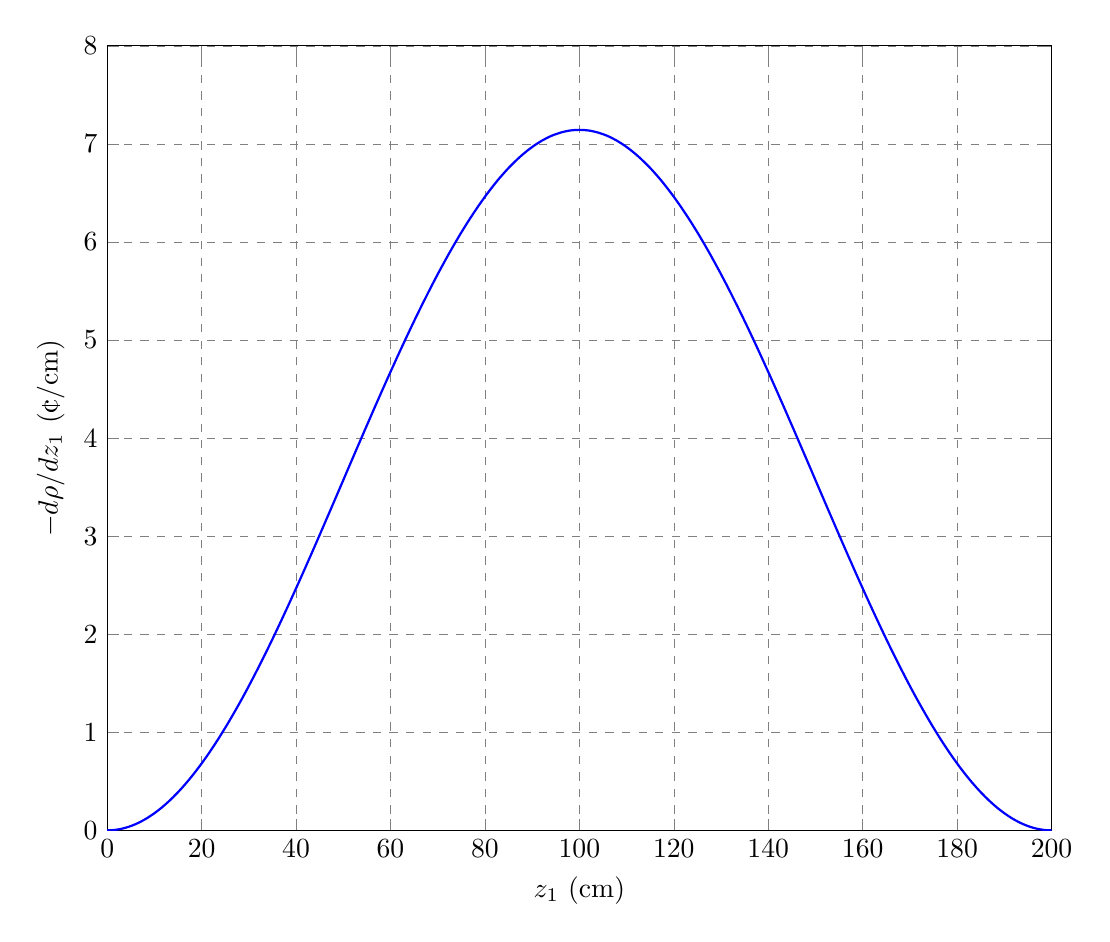
\begin{tikzpicture} \begin{axis}
[scale=1.75, 
 xmin=0, xmax=200,
 ymin=0, ymax=8,
 grid=major, 
 major grid style={color=gray,line width=0.2pt, dashed},
 xlabel=$z_1$ (cm),
 ylabel=$-d\rho/dz_1$ (\textcent/cm),
]

\addplot[line width=0.8pt, color=blue] coordinates {
(   0.0 , 0.000e+00 ) (   0.5 , 4.406e-04 ) (   1.0 , 1.762e-03 ) (   1.5 , 3.965e-03 ) (   2.0 , 7.047e-03 ) (   2.5 , 1.101e-02 ) (   3.0 , 1.585e-02 ) (   3.5 , 2.157e-02 ) (   4.0 , 2.816e-02 ) (   4.5 , 3.563e-02 ) (   5.0 , 4.397e-02 ) (   5.5 , 5.318e-02 ) (   6.0 , 6.326e-02 ) (   6.5 , 7.420e-02 ) (   7.0 , 8.601e-02 ) (   7.5 , 9.868e-02 ) (   8.0 , 1.122e-01 ) (   8.5 , 1.266e-01 ) (   9.0 , 1.418e-01 ) (   9.5 , 1.579e-01 ) (  10.0 , 1.748e-01 ) (  10.5 , 1.926e-01 ) (  11.0 , 2.111e-01 ) (  11.5 , 2.306e-01 ) (  12.0 , 2.508e-01 ) (  12.5 , 2.719e-01 ) (  13.0 , 2.937e-01 ) (  13.5 , 3.164e-01 ) (  14.0 , 3.399e-01 ) (  14.5 , 3.642e-01 ) (  15.0 , 3.893e-01 ) (  15.5 , 4.151e-01 ) (  16.0 , 4.418e-01 ) (  16.5 , 4.692e-01 ) (  17.0 , 4.973e-01 ) (  17.5 , 5.263e-01 ) (  18.0 , 5.560e-01 ) (  18.5 , 5.864e-01 ) (  19.0 , 6.176e-01 ) (  19.5 , 6.495e-01 ) (  20.0 , 6.821e-01 ) (  20.5 , 7.154e-01 ) (  21.0 , 7.494e-01 ) (  21.5 , 7.842e-01 ) (  22.0 , 8.196e-01 ) (  22.5 , 8.557e-01 ) (  23.0 , 8.925e-01 ) (  23.5 , 9.299e-01 ) (  24.0 , 9.680e-01 ) (  24.5 , 1.007e+00 ) (  25.0 , 1.046e+00 ) (  25.5 , 1.086e+00 ) (  26.0 , 1.127e+00 ) (  26.5 , 1.168e+00 ) (  27.0 , 1.210e+00 ) (  27.5 , 1.252e+00 ) (  28.0 , 1.295e+00 ) (  28.5 , 1.338e+00 ) (  29.0 , 1.382e+00 ) (  29.5 , 1.427e+00 ) (  30.0 , 1.472e+00 ) (  30.5 , 1.518e+00 ) (  31.0 , 1.564e+00 ) (  31.5 , 1.611e+00 ) (  32.0 , 1.658e+00 ) (  32.5 , 1.705e+00 ) (  33.0 , 1.753e+00 ) (  33.5 , 1.802e+00 ) (  34.0 , 1.851e+00 ) (  34.5 , 1.900e+00 ) (  35.0 , 1.950e+00 ) (  35.5 , 2.000e+00 ) (  36.0 , 2.051e+00 ) (  36.5 , 2.102e+00 ) (  37.0 , 2.153e+00 ) (  37.5 , 2.205e+00 ) (  38.0 , 2.257e+00 ) (  38.5 , 2.309e+00 ) (  39.0 , 2.362e+00 ) (  39.5 , 2.415e+00 ) (  40.0 , 2.468e+00 ) (  40.5 , 2.521e+00 ) (  41.0 , 2.575e+00 ) (  41.5 , 2.629e+00 ) (  42.0 , 2.683e+00 ) (  42.5 , 2.738e+00 ) (  43.0 , 2.792e+00 ) (  43.5 , 2.847e+00 ) (  44.0 , 2.902e+00 ) (  44.5 , 2.957e+00 ) (  45.0 , 3.013e+00 ) (  45.5 , 3.068e+00 ) (  46.0 , 3.124e+00 ) (  46.5 , 3.180e+00 ) (  47.0 , 3.235e+00 ) (  47.5 , 3.291e+00 ) (  48.0 , 3.347e+00 ) (  48.5 , 3.403e+00 ) (  49.0 , 3.459e+00 ) (  49.5 , 3.515e+00 ) (  50.0 , 3.571e+00 ) (  50.5 , 3.628e+00 ) (  51.0 , 3.684e+00 ) (  51.5 , 3.740e+00 ) (  52.0 , 3.796e+00 ) (  52.5 , 3.852e+00 ) (  53.0 , 3.908e+00 ) (  53.5 , 3.963e+00 ) (  54.0 , 4.019e+00 ) (  54.5 , 4.075e+00 ) (  55.0 , 4.130e+00 ) (  55.5 , 4.185e+00 ) (  56.0 , 4.241e+00 ) (  56.5 , 4.296e+00 ) (  57.0 , 4.351e+00 ) (  57.5 , 4.405e+00 ) (  58.0 , 4.460e+00 ) (  58.5 , 4.514e+00 ) (  59.0 , 4.568e+00 ) (  59.5 , 4.622e+00 ) (  60.0 , 4.675e+00 ) (  60.5 , 4.728e+00 ) (  61.0 , 4.781e+00 ) (  61.5 , 4.834e+00 ) (  62.0 , 4.886e+00 ) (  62.5 , 4.938e+00 ) (  63.0 , 4.990e+00 ) (  63.5 , 5.041e+00 ) (  64.0 , 5.092e+00 ) (  64.5 , 5.143e+00 ) (  65.0 , 5.193e+00 ) (  65.5 , 5.243e+00 ) (  66.0 , 5.292e+00 ) (  66.5 , 5.341e+00 ) (  67.0 , 5.389e+00 ) (  67.5 , 5.437e+00 ) (  68.0 , 5.485e+00 ) (  68.5 , 5.532e+00 ) (  69.0 , 5.579e+00 ) (  69.5 , 5.625e+00 ) (  70.0 , 5.671e+00 ) (  70.5 , 5.716e+00 ) (  71.0 , 5.760e+00 ) (  71.5 , 5.804e+00 ) (  72.0 , 5.848e+00 ) (  72.5 , 5.891e+00 ) (  73.0 , 5.933e+00 ) (  73.5 , 5.975e+00 ) (  74.0 , 6.016e+00 ) (  74.5 , 6.057e+00 ) (  75.0 , 6.097e+00 ) (  75.5 , 6.136e+00 ) (  76.0 , 6.175e+00 ) (  76.5 , 6.213e+00 ) (  77.0 , 6.250e+00 ) (  77.5 , 6.287e+00 ) (  78.0 , 6.323e+00 ) (  78.5 , 6.359e+00 ) (  79.0 , 6.393e+00 ) (  79.5 , 6.427e+00 ) (  80.0 , 6.461e+00 ) (  80.5 , 6.493e+00 ) (  81.0 , 6.525e+00 ) (  81.5 , 6.556e+00 ) (  82.0 , 6.587e+00 ) (  82.5 , 6.617e+00 ) (  83.0 , 6.646e+00 ) (  83.5 , 6.674e+00 ) (  84.0 , 6.701e+00 ) (  84.5 , 6.728e+00 ) (  85.0 , 6.754e+00 ) (  85.5 , 6.779e+00 ) (  86.0 , 6.803e+00 ) (  86.5 , 6.826e+00 ) (  87.0 , 6.849e+00 ) (  87.5 , 6.871e+00 ) (  88.0 , 6.892e+00 ) (  88.5 , 6.912e+00 ) (  89.0 , 6.932e+00 ) (  89.5 , 6.950e+00 ) (  90.0 , 6.968e+00 ) (  90.5 , 6.985e+00 ) (  91.0 , 7.001e+00 ) (  91.5 , 7.016e+00 ) (  92.0 , 7.031e+00 ) (  92.5 , 7.044e+00 ) (  93.0 , 7.057e+00 ) (  93.5 , 7.069e+00 ) (  94.0 , 7.080e+00 ) (  94.5 , 7.090e+00 ) (  95.0 , 7.099e+00 ) (  95.5 , 7.107e+00 ) (  96.0 , 7.115e+00 ) (  96.5 , 7.121e+00 ) (  97.0 , 7.127e+00 ) (  97.5 , 7.132e+00 ) (  98.0 , 7.136e+00 ) (  98.5 , 7.139e+00 ) (  99.0 , 7.141e+00 ) (  99.5 , 7.142e+00 ) ( 100.0 , 7.143e+00 ) ( 100.5 , 7.142e+00 ) ( 101.0 , 7.141e+00 ) ( 101.5 , 7.139e+00 ) ( 102.0 , 7.136e+00 ) ( 102.5 , 7.132e+00 ) ( 103.0 , 7.127e+00 ) ( 103.5 , 7.121e+00 ) ( 104.0 , 7.115e+00 ) ( 104.5 , 7.107e+00 ) ( 105.0 , 7.099e+00 ) ( 105.5 , 7.090e+00 ) ( 106.0 , 7.080e+00 ) ( 106.5 , 7.069e+00 ) ( 107.0 , 7.057e+00 ) ( 107.5 , 7.044e+00 ) ( 108.0 , 7.031e+00 ) ( 108.5 , 7.016e+00 ) ( 109.0 , 7.001e+00 ) ( 109.5 , 6.985e+00 ) ( 110.0 , 6.968e+00 ) ( 110.5 , 6.950e+00 ) ( 111.0 , 6.932e+00 ) ( 111.5 , 6.912e+00 ) ( 112.0 , 6.892e+00 ) ( 112.5 , 6.871e+00 ) ( 113.0 , 6.849e+00 ) ( 113.5 , 6.826e+00 ) ( 114.0 , 6.803e+00 ) ( 114.5 , 6.779e+00 ) ( 115.0 , 6.754e+00 ) ( 115.5 , 6.728e+00 ) ( 116.0 , 6.701e+00 ) ( 116.5 , 6.674e+00 ) ( 117.0 , 6.646e+00 ) ( 117.5 , 6.617e+00 ) ( 118.0 , 6.587e+00 ) ( 118.5 , 6.556e+00 ) ( 119.0 , 6.525e+00 ) ( 119.5 , 6.493e+00 ) ( 120.0 , 6.461e+00 ) ( 120.5 , 6.427e+00 ) ( 121.0 , 6.393e+00 ) ( 121.5 , 6.359e+00 ) ( 122.0 , 6.323e+00 ) ( 122.5 , 6.287e+00 ) ( 123.0 , 6.250e+00 ) ( 123.5 , 6.213e+00 ) ( 124.0 , 6.175e+00 ) ( 124.5 , 6.136e+00 ) ( 125.0 , 6.097e+00 ) ( 125.5 , 6.057e+00 ) ( 126.0 , 6.016e+00 ) ( 126.5 , 5.975e+00 ) ( 127.0 , 5.933e+00 ) ( 127.5 , 5.891e+00 ) ( 128.0 , 5.848e+00 ) ( 128.5 , 5.804e+00 ) ( 129.0 , 5.760e+00 ) ( 129.5 , 5.716e+00 ) ( 130.0 , 5.671e+00 ) ( 130.5 , 5.625e+00 ) ( 131.0 , 5.579e+00 ) ( 131.5 , 5.532e+00 ) ( 132.0 , 5.485e+00 ) ( 132.5 , 5.437e+00 ) ( 133.0 , 5.389e+00 ) ( 133.5 , 5.341e+00 ) ( 134.0 , 5.292e+00 ) ( 134.5 , 5.243e+00 ) ( 135.0 , 5.193e+00 ) ( 135.5 , 5.143e+00 ) ( 136.0 , 5.092e+00 ) ( 136.5 , 5.041e+00 ) ( 137.0 , 4.990e+00 ) ( 137.5 , 4.938e+00 ) ( 138.0 , 4.886e+00 ) ( 138.5 , 4.834e+00 ) ( 139.0 , 4.781e+00 ) ( 139.5 , 4.728e+00 ) ( 140.0 , 4.675e+00 ) ( 140.5 , 4.622e+00 ) ( 141.0 , 4.568e+00 ) ( 141.5 , 4.514e+00 ) ( 142.0 , 4.460e+00 ) ( 142.5 , 4.405e+00 ) ( 143.0 , 4.351e+00 ) ( 143.5 , 4.296e+00 ) ( 144.0 , 4.241e+00 ) ( 144.5 , 4.185e+00 ) ( 145.0 , 4.130e+00 ) ( 145.5 , 4.075e+00 ) ( 146.0 , 4.019e+00 ) ( 146.5 , 3.963e+00 ) ( 147.0 , 3.908e+00 ) ( 147.5 , 3.852e+00 ) ( 148.0 , 3.796e+00 ) ( 148.5 , 3.740e+00 ) ( 149.0 , 3.684e+00 ) ( 149.5 , 3.628e+00 ) ( 150.0 , 3.571e+00 ) ( 150.5 , 3.515e+00 ) ( 151.0 , 3.459e+00 ) ( 151.5 , 3.403e+00 ) ( 152.0 , 3.347e+00 ) ( 152.5 , 3.291e+00 ) ( 153.0 , 3.235e+00 ) ( 153.5 , 3.180e+00 ) ( 154.0 , 3.124e+00 ) ( 154.5 , 3.068e+00 ) ( 155.0 , 3.013e+00 ) ( 155.5 , 2.957e+00 ) ( 156.0 , 2.902e+00 ) ( 156.5 , 2.847e+00 ) ( 157.0 , 2.792e+00 ) ( 157.5 , 2.738e+00 ) ( 158.0 , 2.683e+00 ) ( 158.5 , 2.629e+00 ) ( 159.0 , 2.575e+00 ) ( 159.5 , 2.521e+00 ) ( 160.0 , 2.468e+00 ) ( 160.5 , 2.415e+00 ) ( 161.0 , 2.362e+00 ) ( 161.5 , 2.309e+00 ) ( 162.0 , 2.257e+00 ) ( 162.5 , 2.205e+00 ) ( 163.0 , 2.153e+00 ) ( 163.5 , 2.102e+00 ) ( 164.0 , 2.051e+00 ) ( 164.5 , 2.000e+00 ) ( 165.0 , 1.950e+00 ) ( 165.5 , 1.900e+00 ) ( 166.0 , 1.851e+00 ) ( 166.5 , 1.802e+00 ) ( 167.0 , 1.753e+00 ) ( 167.5 , 1.705e+00 ) ( 168.0 , 1.658e+00 ) ( 168.5 , 1.611e+00 ) ( 169.0 , 1.564e+00 ) ( 169.5 , 1.518e+00 ) ( 170.0 , 1.472e+00 ) ( 170.5 , 1.427e+00 ) ( 171.0 , 1.382e+00 ) ( 171.5 , 1.338e+00 ) ( 172.0 , 1.295e+00 ) ( 172.5 , 1.252e+00 ) ( 173.0 , 1.210e+00 ) ( 173.5 , 1.168e+00 ) ( 174.0 , 1.127e+00 ) ( 174.5 , 1.086e+00 ) ( 175.0 , 1.046e+00 ) ( 175.5 , 1.007e+00 ) ( 176.0 , 9.680e-01 ) ( 176.5 , 9.299e-01 ) ( 177.0 , 8.925e-01 ) ( 177.5 , 8.557e-01 ) ( 178.0 , 8.196e-01 ) ( 178.5 , 7.842e-01 ) ( 179.0 , 7.494e-01 ) ( 179.5 , 7.154e-01 ) ( 180.0 , 6.821e-01 ) ( 180.5 , 6.495e-01 ) ( 181.0 , 6.176e-01 ) ( 181.5 , 5.864e-01 ) ( 182.0 , 5.560e-01 ) ( 182.5 , 5.263e-01 ) ( 183.0 , 4.973e-01 ) ( 183.5 , 4.692e-01 ) ( 184.0 , 4.418e-01 ) ( 184.5 , 4.151e-01 ) ( 185.0 , 3.893e-01 ) ( 185.5 , 3.642e-01 ) ( 186.0 , 3.399e-01 ) ( 186.5 , 3.164e-01 ) ( 187.0 , 2.937e-01 ) ( 187.5 , 2.719e-01 ) ( 188.0 , 2.508e-01 ) ( 188.5 , 2.306e-01 ) ( 189.0 , 2.111e-01 ) ( 189.5 , 1.926e-01 ) ( 190.0 , 1.748e-01 ) ( 190.5 , 1.579e-01 ) ( 191.0 , 1.418e-01 ) ( 191.5 , 1.266e-01 ) ( 192.0 , 1.122e-01 ) ( 192.5 , 9.868e-02 ) ( 193.0 , 8.601e-02 ) ( 193.5 , 7.420e-02 ) ( 194.0 , 6.326e-02 ) ( 194.5 , 5.318e-02 ) ( 195.0 , 4.397e-02 ) ( 195.5 , 3.563e-02 ) ( 196.0 , 2.816e-02 ) ( 196.5 , 2.157e-02 ) ( 197.0 , 1.585e-02 ) ( 197.5 , 1.101e-02 ) ( 198.0 , 7.047e-03 ) ( 198.5 , 3.965e-03 ) ( 199.0 , 1.762e-03 ) ( 199.5 , 4.406e-04 ) ( 200.0 , 0.000e+00 ) 
};

%\legend{Fuel,Moderator}
\end{axis}
\end{tikzpicture}
\caption{Differential control rod insertion curve.}
 \label{Fig:kinetics_differentialControlRodInsertion}
\end{center}
\end{figure}

To illustrate this, let us suppose that $H = 200$~cm and $\Delta_a = 0.05$~cm$^{-1}$, and $\nu\Sigma_f = 1.0$~cm$^{-1}$. If we take the effective delayed neutron fraction $\beta = 0.007$. We can compute the differential control rod worth in \textcent of reactivity per unit insertion. This is displayed in Fig.~\ref{Fig:kinetics_differentialControlRodInsertion}. Because the reactor is symmetric, we see the differential control rod worth curve is also symmetric. It is also maximized at the center of the core. This is intuitive because in there are more neutrons in the center of the core and these neutrons are more important (less likely to leak out) than those on the perifery.

\subsection{Point Kinetics Model Revisited}

Now that we have the adjoint function, we can more rigorously define the point kinetics equation to account of spatial and energy variations in an average sense. It turns out the final result has exactly the same where the coefficients have a different definition involving adjoint weighting.

To begin, we start with the time-dependent neutron transport equation with precursors from Eqs.~\eqref{Eq:kinetics_timeDependentTransportEquationsPrecursors} and using operator notation:
\begin{align}
  &\frac{1}{v}\dho{\psi}{t} + \mathcal{M} \psi(\pos,\dir,E,t) \nonumber \\*
  &= \mathcal{F}_p \psi(\pos,\dir,E,t) + \sum_i \frac{\chi_i(E)}{4\pi} \lambda_i C_i(\pos,t) + Q(\pos,\dir,E) , \nonumber \\*
  &\dho{C_i}{t} = - \lambda_i C_i(\pos,t) + \mathcal{B}_i \psi(\pos,\dir,E,t) . \nonumber
\end{align}
Next, we assume that the space, direction, and energy dependencies are completely separable from the time dependence:
\begin{subequations}
\begin{align}
  \psi(\pos,\dir,E,t) \approx \Psi(\pos,\dir,E) p(t), \\
  C_i(\pos,\dir,E,t) \approx \Xi_i(\pos,\dir,E) \overline{C}_i(t). 
\end{align}
\end{subequations}
Inserting this into the equation gives
\begin{subequations}
\begin{align}
  &\frac{\Psi}{v}\frac{dp}{dt}  +   \mathcal{M} \Psi p(t) \nonumber \\*
  &= \mathcal{F}_p \Psi p(t)  + \sum_i \Xi_i \frac{\chi_i(E)}{4\pi} \lambda_i \overline{C}_i(t) + Q ,  \label{Eq:kinetics_pointKineticsDerivationAdjoint_NeutronBalance_step0} \\*
  &\Xi_i \frac{ d\overline{C}_i}{dt} = - \Xi_i  \lambda_i \overline{C}_i(t) +  \mathcal{B}_i \Psi p(t). \label{Eq:kinetics_pointKineticsDerivationAdjoint_PrecursorBalance_step0}
\end{align}
\end{subequations}

We then add and subtract the delayed neutron source to the right-hand side of the neutron balance equation and combine the prompt plus delayed fission sources. This becomes
\begin{align}
  &\frac{\Psi}{v}\frac{dp}{dt}  +   \mathcal{M} \Psi p(t) \nonumber \\*
  &= \mathcal{F} \Psi  p(t) - \sum_i \frac{\chi_i}{4\pi} \mathcal{B}_i \Psi  p(t) + \sum_i \Xi_i \frac{\chi_i(E)}{4\pi} \lambda_i \overline{C}_i(\pos,t) + Q . \label{Eq:kinetics_pointKineticsDerivationAdjoint_NeutronBalance_step1}
\end{align}
Next we multiply by the adjoint function of the shape function $\Psi^\dagger$ and integrate over the all volume, directions, and energy:
\begin{align}
  &\left< \Psi^\dagger, \frac{1}{v} \Psi \right> \frac{dp}{dt}   +  \left< \Psi^\dagger, \mathcal{M} \Psi \right> p(t) \nonumber \\*
  &= \left< \Psi^\dagger, \mathcal{F} \Psi \right>  p(t) - \sum_i \left< \Psi^\dagger, \frac{\chi_i}{4\pi} \mathcal{B}_i \Psi \right>   p(t) + \sum_i \left< \Psi^\dagger, \frac{\chi_i(E)}{4\pi} \lambda_i \Xi_i \right> \overline{C}_i(t) + \left< \Psi^\dagger, Q \right>. \label{Eq:kinetics_pointKineticsDerivationAdjoint_NeutronBalance_step2}
\end{align}

Then, we write down the steady-state adjoint neutron transport equation for the shape function from Eq.~\eqref{Eq:kinetics_AdjointTransportKEigenvalueOperator},
\begin{align}
  \mathcal{M}^\dagger \Psi^\dagger = \frac{1}{k} \mathcal{F}^\dagger \Psi^\dagger , \nonumber
\end{align}
multiply by the shape function $\Psi$, and integrate over all positions, directions, and energy in the reactor. This gives
\begin{align}
  \left< \Psi, \mathcal{M}^\dagger \Psi^\dagger \right> = \frac{1}{k} \left< \Psi, \mathcal{F}^\dagger \Psi^\dagger \right> . \nonumber
\end{align}
However, applying the identity in Eq.~\eqref{Eq:kinetics_forwardAdjointNoBoundaryIdentity}, we have
\begin{align}
  \left< \Psi^\dagger, \mathcal{M} \Psi \right> = \frac{1}{k} \left< \Psi^\dagger, \mathcal{F} \Psi \right> .
\end{align}
Then, we multiply this equation by $p(t)$ and subtract this from the balance equation Eq.~\eqref{Eq:kinetics_pointKineticsDerivationAdjoint_NeutronBalance_step2}. We notice that the net migration term cancels out. We then divide by the coefficient on the time derivative on the left-hand side and get
\begin{align}
   \frac{dp}{dt}  
  &=  \left( 1 - \frac{1}{k} \right) \dfrac{ \left< \Psi^\dagger, \mathcal{F} \Psi \right> }{ \left< \Psi^\dagger, \frac{1}{v} \Psi \right> } p(t)  - \sum_i \dfrac{ \left< \Psi^\dagger, \frac{\chi_i}{4\pi} \mathcal{B}_i \Psi \right> }{ \left< \Psi^\dagger, \frac{1}{v} \Psi \right> }  p(t) \nonumber \\*
  &+ \sum_i \dfrac{ \left< \Psi^\dagger, \frac{\chi_i(E)}{4\pi} \lambda_i \Xi_i \right> }{ \left< \Psi^\dagger, \frac{1}{v} \Psi \right> } \overline{C}_i(t) + \dfrac{ \left< \Psi^\dagger, Q \right> }{ \left< \Psi^\dagger, \frac{1}{v} \Psi \right> }. \label{Eq:kinetics_pointKineticsDerivationAdjoint_NeutronBalance_step3}
\end{align}

We note that reactivity is
\begin{align}
  \rho = 1 - \frac{1}{k} . \nonumber
\end{align}
We then define the \emph{effective} neutron generation time,
\begin{subequations} \label{Eq:kinetics_pointKineticsParameters_AdjointWeighted}
\begin{align}
  \Lambda_\eff = \dfrac{ \left< \Psi^\dagger, \frac{1}{v} \Psi  \right> }{ \left< \Psi^\dagger, \mathcal{F} \Psi \right> } ,
\end{align}
the \emph{effective} delayed neutron fraction for the $i$th precursor group
\begin{align}
  \beta_{\eff,i} = \dfrac{ \left< \Psi^\dagger, \frac{\chi_i}{4\pi} \mathcal{B}_i \Psi  \right> }{ \left< \Psi^\dagger, \mathcal{F} \Psi \right> } ,
\end{align}
the adjoint-weighted precursor concentration
\begin{align}
  \zeta_i(t) = \dfrac{ \left< \Psi^\dagger, \frac{\chi_i(E)}{4\pi} \Xi_i \right> }{ \left< \Psi^\dagger, \mathcal{F} \Psi \right> } \overline{C}_i(t) ,
\end{align}
and the adjoint-weighted source
\begin{align}
  s(t) = \dfrac{ \left< \Psi^\dagger, Q \right> }{ \left< \Psi^\dagger, \mathcal{F}  \Psi \right> }.
\end{align}
\end{subequations}
Applying these definitions and that $\beta_{\eff} = \sum_i \beta_{\eff,i}$, we get the point kinetics equations using the effective or adjoint-weighted parameters:
\begin{align}
  \frac{dp}{dt} = \left( \frac{ \rho - \beta_\eff }{ \Lambda_\eff } \right) p(t) + \frac{1}{\Lambda_\eff} \sum_i \lambda_i \zeta_i(t) + \frac{1}{\Lambda_\eff} s(t) .
\end{align}

Obtaining the precursor balance equation proceeds similarly. We first take Eq.~\eqref{Eq:kinetics_pointKineticsDerivationAdjoint_PrecursorBalance_step0} for the separated precursor equation and multiply it by $\Psi^\dagger \chi_i/4\pi$ and integrate over all positions, directions, and energies, to get
\begin{align}
  \left< \Psi^\dagger , \frac{\chi_i}{4\pi} \Xi_i \right> \frac{ d\overline{C}_i}{dt} = -\lambda_i   \left< \Psi^\dagger , \frac{\chi_i}{4\pi}  \Xi_i \right> \overline{C}_i(t) +  \left< \Psi^\dagger, \frac{\chi_i}{4\pi} \mathcal{B}_i \Psi \right> p(t)
\end{align}
We then divide by the adjoint-weighted fission source $\left< \Psi^\dagger, \mathcal{F} \Psi \right>$,
\begin{align}
  \frac{d}{dt} \dfrac{ \left< \Psi^\dagger , \frac{\chi_i}{4\pi} \Xi_i \right> }{ \left< \Psi^\dagger, \mathcal{F} \Psi \right> }  \overline{C}_i
 = -\lambda_i   \dfrac{ \left< \Psi^\dagger , \frac{\chi_i}{4\pi} \Xi_i \right> }{ \left< \Psi^\dagger, \mathcal{F} \Psi \right> } \overline{C}_i(t) 
 +  \dfrac{ \left< \Psi^\dagger, \frac{\chi_i}{4\pi} \mathcal{B}_i \Psi \right> }{  \left< \Psi^\dagger, \mathcal{F} \Psi \right> }  p(t) .
\end{align}
Finally we apply the definitions of the adjoint-weighted precursors and the effective delayed neutron fraction for the $i$th precursor group to obtain the final result of
\begin{align}
  \frac{d\zeta_i}{dt} = -\lambda_i \zeta_i(t) + \beta_{\eff,i} p(t) .
\end{align}

This completes the formal derivation. The point kinetics equations are identical to those we obtained earlier except the kinetics parameters have been replaced by the effective values and $\zeta_i(t)$ and $s(t)$ are defined a bit differently with adjoint functions. These new definitions are in Eq.~\eqref{Eq:kinetics_pointKineticsParameters_AdjointWeighted}. Using these alternative definitions yields a greater consistency with the continuous-energy or multigroup transport or diffusion equations, whereas the one-speed versions are correct, but leave out essential details.

For example, the energy dependence of the delayed neutron emission tends to increase the importance of delayed neutrons and therefore the effective delayed neutron fraction is greater than what would be predicted from a simple treatment. The reason is because lower energy neutrons in a thermal reactor are less likely to leak out and therefore more likely to cause fission and drive the chain reaction forward, in accordance with the interpretation of neutron importance. 

Another realization of this is in molten-salted fueled reactors. In these systems, delayed precursors are produced within the reactor but are advected after their creation. On balance the precursors tend to decay at lower importance regions than where they were initially created. This implies the effective delayed neutron factor tends to be smaller than for an equivalent reactor where the fuel is stationary. This reduction is vital to consider the boundary between delayed and prompt supercritical reactivities.

Another situation is the effective neutron generation time in a small metal system that is reflected by a large moderating reflector. In such as case, a neutron will can traverse far into the reflector and spend a large amount of time but be so far away from the actual fissile material so as not to matter with respect to the chain reaction. A simplistic calculation will grossly overestimate the effective neutron generation time (sometimes by orders of magnitude).



\section{Reactor Feedback and Control}

Thus far we solved the point kinetics equations in the absence of any feedback mechanisms. Of course, increasing the power increases the temperature, and this impacts the nuclear and material properties, which then impacts the kinetics equations. The purpose of this section is to describe the relevant \emph{natural} mechanisms, which we call here feedback. This contrasts with those that are externally imposed by an operator, which we classify as control mechanisms.

\subsection{Characterization of Natural Feedback Mechanisms}

Natural feedback mechanisms are inherent in the physics of an operating nuclear reactor and are therefore independent of any human intervention and can be completely relied upon to occur. As such, we often rely on these phenomena to provide inherent safety in the design, or we engineer the reactor in a way to mitigate or eliminate such mechanisms that may be detrimental to the operational safety of the reactor. In terms of feedback mechanisms, we can group into four distinct timescales:
\begin{enumerate}
  \item Immediate or prompt feedback. These occur on the timescale of the prompt neutron generation time $\Lambda$ or shorter. The most prominent example in reactor analysis is Doppler broadening, which is direct consequence of thermal motion and temperature and is therefore literally instantaneous with any rise in temperature. In small metal systems such as fast burst reactors or possibly space reactors where leakage is a major loss mechanism, thermal expansion effectively falls into this category; however, for metal-fueled reactors, such as sodium-cooled fast reactors that are large in size and especially thermal oxide fueled reactors, the heat transfer requires more time and is often in the next category.
  \item Short-term feedback. This feedback is on the same timescale of the delayed neutron precursors, milliseconds to minutes. Typically these feedback mechanisms are those related to the transfer of thermal energy via conduction or convection from the fuel into other parts of the reactor such as the coolant or moderator.
  \item Medium-term feedback. This timescale is on the hours to days timescale. The most important mechanism in this regime for thermal reactors is the buildup of a couple strongly absorbing fission products, namely $^{135}$I and $^{135}$Xe that have a major impact on the reactivity and in certain large reactors can lead to spatial oscillations that must be designed around or managed during operations.
  \item Long-term feedback. This is on the timescale of weeks, months, or even years depending on the design. This is in the form of the depletion of fuel, burnable absorbers placed in the reactor for long-term reactivity control, or the conversion of fertile isotopes into fissile ones, e.g., the buildup of $^{239}$Pu in light-water reactors.
\end{enumerate}

Which feedback mechanisms matter and by how much is strongly dependent on the reactor design. Much of this discussion focuses on conventional light-water reactors, for which the natural feedback mechanisms are well characterized in terms of them being positive or negative and a small number of them dominate. On the immediate to short time scales, these are Doppler feedback in the fuel and the moderator density effects. On longer timescales, the buildup of $^{135}$Xe becomes a concern as well as the depletion of fuel and burnable absorbers or the conversion of fertile isotopes.

Fast reactors, on the other hand, are a bit tricker on the immediate to short timescale because individual mechanisms tend to be small and whether they add or subtract from the reactivity is less obvious. In a sense, grappling with the various offsetting natural feedback mechanisms and ensuring the inherent safety of a particular fast reactor design is more challenging. Conversely, the buildup of $^{135}$Xe is largely irrelevant to the fast spectrum, so these issues are absent there. However, on longer time scales, fast reactors are often used for to create new fuel from fertile material (conversion or breeding) or leverage the fast spectrum to burn long-lived transuranic isotopes that create a radiotoxicity burden for long-term spent fuel management.

\subsection{Reactor Control Mechanisms}

Reactor control mechanisms are ways that an operator can insert positive or negative reactivity into a reactor. There are three broad types:
\begin{enumerate}
  \item Movable control elements. Usually these are strong neutron absorbers that can be inserted or removed from the reactor. In pressurized water reactors these are in the form of control rods that are inserted from the top of the reactor and consist of an allow of silver, indium, and cadmium. 
  
  In boiling water reactors, these are blades inserted from the bottom made of boron, which is a much stronger neutron absorber. The reason for the bottom insertion in a boiling water reactor is because the moderator is mostly in a liquid or low-quality steam phase and the neutron spectrum is quite thermal in contrast to the top of the core where the moderator is low-density, high-quality steam and therefore much less moderation. 
  
  In microreactors or space reactors, these movable control elements can take the form of movable reflectors or drums that increase reactivity. 
  
  The advantage of movable control elements is they are mechanical in nature and can quickly (on the seconds timescale) be used to vary the reactivity or shutdown the reactor if needed. The disadvantage is that their use leads to localized perturbations in the neutron flux that distorts the flux shape and leads to increased peaking. Conversely, control elements can be used to mitigate peaking as well. Peaking effects are problematic because the limiting factor is based on the peak power, not merely the average.
  
  \item Chemical shims or soluble poisons. This mechanism is primarily used only in pressurized water reactors. Boron is a strong neutron absorber that can be put dissolved into the water moderator/coolant by way of boric acid. The boron concentration is controlled through chemical means.
  
  The advantage to a chemical shim is that they uniformly dissolved in the coolant and therefore do not lead to peaking effects endemic to movable control elements. In this sense, an operator can fine tune the reactivity globally, hence the use of the word ``shim''. The major disadvantage is that manipulating the boron concentration through chemical means is a much more time consuming process and therefore cannot be practically used to shutdown the reactor. Furthermore, its use is rather limited to the pressurized water reactor design.
  
  \item Fixed burnable absorbers. These are solid neutron absorbers that are put into the assemblies and loaded in during fueling. These cannot be moved or changed during operations. 
  
  These can be separate elements, such as boron plates that act as curtains between fuel assembles that can be removed during refueling. Another is called wet-annular burnable absorbers (WABAs) that are separated from the fuel and are inserted in guide tubes during fabrication. These two strategies are most used in boiling water reactors.
  
  In pressurized water reactors, burnable absorbers tend to be integrated with the fuel. One option uses rare-earth elements, which tend to have high neutron capture cross sections, baked into certain fuel pellets. The most common is gadolinium oxide (Gd$_2$O$_3$). The other is integral fuel burnable absorbers (IFBA), which is a very thin ZrB$_2$ coating placed onto the fuel pin that shields the fuel from neutrons early the fueling cycle.
  
  The advantage of burnable absorbers is that they do not require human intervention during operations and are therefore a reliable type of feedback mechanism. Used appropriately they can tailor the neutron spectrum and distribution locally throughout a fueling cycle. Their drawback is they are fixed and once they are installed, cannot be changed during operation.
\end{enumerate}

\subsection{Reactor Startup and Reactivity Defects}

The discussion on reactor feedback and control must really be done in connection to how a reactor is brought from shutdown to full power operations, as there are key concepts and terminology that derive from this. Here we focus primarily on pressurized water reactors.

Initially or after an extended period of being offline because of refueling or repairs, a reactor and the surrounding energy conversion and safety systems are is in a \emph{cold shutdown} state. The first step is to bring the reactor from this cold state to what is termed \emph{hot-zero power} or hot standby. In this state, the reactor is at about 1\% of its full power level with coolant inlet temperatures and pressures near operating conditions. Bringing the reactor from cold shutdown is usually done using external energy sources, most commonly with the reactor coolant pumps, which produce a large amount (a few megawatts) of heat when they operate.

There are a few reasons that the reactor cannot be immediately brought up to full power from cold shutdown. The first is based on the fact that a reactor has large and complex machinery around it to support the removal of a vast amount of thermal energy. A rapid rise in power could potentially damage this machinery or exceed its ability to remove heat if it is not brought into operating conditions. Another is that the reactor and the machinery needs to undergo tests and checks to ensure it is operating correctly before there is too much power to remove. Additionally, the reactor can be brought up to criticality slowly and safely in this condition by the removal of control elements or soluble boron. Finally, at low temperatures the reactor can be in a condition (because of soluble boron in the moderator) with positive feedback, where an increase in temperature would lead to an increase in reactivity, leading to a further and increasingly rapid cycle of temperature and reactivity grows. (We expand on this further in the next sections.) This rapid increase in power could damage the fuel and cladding and is the reason why the reactor is brought into a hot-zero power condition by external means and not through fission. 

What distinguishes the hot-zero-power condition from the hot-full-power condition is that the feedback effects within the reactor for increasing the power up until about 1\% are negligible. There is of course still feedback effects on the reactivity that occur by virtue of raising the temperature of the system to the hot-zero-power condition, but this is of a different character from the perspective of the reactor. We refer to the change in reactivity as the \emph{temperature defect} $\rho_T$. (It is called a defect because it is always negative in any reasonable reactor.)

The fission distribution at hot-zero-power at criticality essentially behaves just as we calculated in the previous chapters. As the reactor is brought from 1\% of full power up to full power, the fuel temperature begins to rise dramatically and localized feedback effects become dominant. In a suitably designed reactor, the feedback loop is negative such that a rise in power tends to decrease the reactivity, so to raise the power the operators have to fight against these effects by inserting positive reactivity through removing control rods or diluting soluble boron in the coolant. Furthermore, localized feedback effects tend to flatten out the fission or power distribution spatially such that they no longer follow the simplified models that apply at hot zero power. The amount of reactivity that must be inserted to go from the hot-zero-power condition to the the hot-full-power condition is referred to as the \emph{power defect} $\rho_P$.

To review the reactivity defects:
\begin{align}
  \rho_T 
  &= \text{temperature defect} \nonumber \\
  &= \text{the inherent change in reactivity between the cold-shutdown and} \nonumber \\
  &\ \ \ \text{ hot-zero-power conditions.} \nonumber \\
  \rho_P
  &= \text{power defect} \nonumber \\
  &= \text{the inherent change in reactivity between the hot-zero-power and} \nonumber \\
  &\ \ \ \text{ hot-full-power conditions.} \nonumber
\end{align}
This implies the reactor at a minimum must have built in enough \emph{excess reactivity} $\rho_{ex}$ available to overcome these defects to even start the reactor. In reality, we need even more because once the reactor turns on additional feedback effects in the form of buildup of fission product poisons and fuel burnup occur. Of course, this excess reactivity must be offset by control mechanisms else the reactor would be in a very supercritical state. Formally, we state
\begin{align}
  \rho_{ex} 
  &= \text{excess reactivity} \nonumber \\
  &= \text{amount of (positive) reactivity available beyond the criticality condition.} \nonumber
\end{align}

\subsection{Temperature and Power Coefficients of Reactivity}

Now that we have discussed the ideas behind reactor feedback and control and how they relate to reactor operations, we need to formalize these ideas mathematically. To begin this, we start with the notion of the differential reactivity, which for a reactor near critical is the differential of the logarithm of $k$. This is
\begin{align}
  d\rho = d\left( 1 - \frac{1}{k} \right) = -d\left( \frac{1}{k} \right) = \frac{dk}{k^2} \approx \frac{dk}{k} = d(\ln k).
\end{align}
For $k \approx 1$, we have that $k^2 \approx k$.

From this we define the temperature coefficient of reactivity,
\begin{align}
  \gamma_T = \frac{d\rho}{dT} \approx \frac{1}{k} \frac{dk}{dT} .
\end{align}
(Most references use $\alpha_T$ for this, but we already have enough things using that Greek letter.) In a light-water reactor, the short-time feedback effects are from fuel Doppler broadening and the moderator density. We therefore, can break the overall temperature coefficient of reactivity into separate coefficients for the fuel and moderator as
\begin{align}
  \gamma_T = \gamma_T^F + \gamma_T^M .
\end{align}

Here the fuel temperature coefficient of reactivity is primarily driven by the change in the resonance escape probability $p$ because of Doppler broadening with other effects such as thermal expansion or changes in the scattering distribution are negligible. The fuel coefficient of reactivity is
\begin{align}
  \gamma_T^F = \frac{1}{k} \frac{dk}{d \overline{T}^F } \approx \frac{1}{p} \frac{dp}{d \overline{T}^F } .
\end{align}
The fuel temperature coefficient in a thermal reactor is almost always negative. The reason is because to thermalize the neutrons must escape highly absorbent low-lying resonances in $^{238}$U that broaden out significantly with increases in temperature. This is good because Doppler broadening is an inherent safety mechanism.

The moderator temperature coefficient of reactivity is primarily driven by the associated change in the density and to a lesser degree by the enhancement of leakage and upscattering (because of increased thermal motion). An increase in temperature has two primary effects. The first is the moderator is optically thinner and therefore neutrons in resonance ranges are less likely to downscatter and escape the resonances. Secondly, the moderator absorbs fewer thermal neutrons and therefore the thermal utilization $f$ is increased. This is described using the chain rule as
\begin{align}
  \gamma_T^M = \frac{1}{k} \frac{dk}{d \overline{T}^M }  \approx \frac{1}{k} \frac{dk}{dN^M} \frac{dN^M}{d \overline{T}^M } ,
\end{align}
and
\begin{align}
  \frac{1}{k} \frac{dk}{dN^M} \approx \frac{1}{p} \frac{dp}{d N^M } + \frac{1}{f} \frac{df}{d N^M } .
\end{align}

Unlike with the fuel Doppler coefficient, the moderator density coefficient could be either negative or positive. Generally speaking, we wish to avoid the latter scenario during regular operations because a positive feedback loop can lead to a rapid runaway in the reactivity and hence core damage. We call the case where the moderator temperature coefficient is negative \emph{undermoderated} and the case where it is positive \emph{overmoderated}. In the design phase of the reactor it is important to select a unit-cell pitch to fuel diameter ratio such that the reactor is undermoderated given ideal conditions. 

This gets complicated by the use of soluble poisons. The more boron dissolved in the moderator, the more absorbent it is, which moves the reactivity coefficient in the positive direction. This effectively limits the amount of soluble boron that can be safely used during normal operations, at least between hot-zero-power and hot-full-power conditions. As mentioned, it is sometimes the case that there is too much soluble boron in the reactor during cold shutdown scenarios where the moderator temperature coefficients would be positive. This necessitates bringing the reactor up to hot-zero-power conditions using external mechanisms versus fission.

The temperature coefficient is useful for quantifying the effect of bringing reactor up to hot-zero-power conditions. We can calculate the temperature defect to the temperature coefficient as
\begin{align}
  \rho_T = \int_{T_{amb}}^{T_{hzp}} \gamma_T(T) dT.
\end{align}
Here $T_{amb}$ is the ambient temperature during cold shutdown and $T_{hzp}$ is the temperature at hot-zero-power, which is typically taken to be about the coolant inlet temperature.

For hot-full-power conditions, the temperature coefficient is not particularly adequate and instead we use the power coefficient of reactivity. We can break this down into fuel and moderator components as
\begin{align}
  \gamma_P = \frac{d\rho}{dP} = \frac{1}{k} \frac{dk}{dP} = \frac{1}{k} \frac{dk}{d\overline{T}^F} \frac{d\overline{T}^F}{dP} + \frac{1}{k} \frac{dk}{d\overline{T}^M} \frac{d\overline{T}^M}{dP} ,
\end{align}
where $P$ is the reactor power. Any permissible design requires that the reactor power coefficient is always negative during any operating condition. If this is not the case, then it would be possible for a sudden runaway reactivity excursion to occur at full power, which could lead to core damage and potentially radiological release. The power defect can be calculated from the power coefficient of reactivity as
\begin{align}
  \rho_P = \int_{0}^{P_{FP}} \gamma_P(P) dP .
\end{align}
Here $P_{FP}$ are the full-power level of the reactor and we take the zero-power level to equal zero. Note that this is a slight approximation, since hot-zero-power conditions are typically at around 1\% operating power, but since $\gamma_P(P)$ is small below this, we can extend the range down to zero without much error.

\subsection{Superprompt Transient with Linear Feedback}

For most practical situations, we cannot obtain a closed-form analytical solution to many transient problems and must rely on numerical techniques. One of the notable exceptions is the case of a superprompt reactivity insertion where the temperature coefficient is approximately constant over the transient---this may be reasonable if the reactor is at zero power and the increase in temperature is not too large during the transient. In either case, it does provide an illustrative model of how these reactivity insertion accidents can proceed. So even if quantitatively it may not fully capture such a transient, it is nonetheless useful to get a good qualitative understanding.

First we introduce some definitions and preliminaries. We first assume a separation of the reactor power as the product of $P_{FP}$, the power level at the hot-full-power condition and the flux amplitude function,
\begin{align}
   P(t) = P_{FP} p(t) .
\end{align}
This is not strictly true because the conversion between flux and power is not constant, but it is fairly reasonable. The change in temperature is then proportional to energy release or time-integral over the power times a conversion factor,
\begin{subequations}
\begin{align}
  \Delta T = C_{IT} \int_0^t \left[ p(t') - p_0 \right] dt' .
\end{align}
Here the integrand is the difference in the flux amplitude versus the initial or nominal value that we take at $t = 0$. This subtraction of $p_0$ in the integrand implies \emph{stationary cooling} where thermal energy is transported out of the fuel. For simplicity, we sometimes remove $p_0$ entirely, 
\begin{align}
  \Delta T \approx C_{IT} \int_0^t  p(t')  dt' ,
\end{align}
\end{subequations}
which implies all energy generated in the fuel raises the temperature, not the incremental amount over nominal power. In this we treat the fuel adiabatically. This is not always justified, but simplifies the mathematics considerably, so we make this simplification here.

The conversion factor $C_{IT}$ is the rate of temperature rise at nominal full-power,
\begin{align}
  C_{IT} = \left( \dho{T}{t} \right)_{P_{FP}},
\end{align}
and has units of temperature per full-power per second or (K/fp-s). 

The unit of ``full power'' or fp is a bit confusing as it is technically dimensionless and arises from the assumed factorization of the power $P(t)$. Typical values for a pressurized water reactor is about 80~K/fp-s and for a boiling water reactor it is about 40~K/fp-s. Here we take $T$ as some representative or average fuel temperature.

In a thermal reactor, the dominant prompt feedback mechanism is resonance Doppler broadening. For a typical light-water reactor, this is on the order of $-0.02$\$/K. It is often convenient to multiply this by the conversion factor $C_{IT}$ to arrive at the energy coefficient
\begin{align}
  \gamma = C_{IT} \gamma_T .
\end{align}
For a pressurized water reactor, this is typically about $-1.6$\$/fp-s.

Next, we analyze the prompt kinetics solution we obtained for a positive reactivity insertion in a critical reactor. Here we consider the case $\rho_1 > \beta$. The flux amplitude is given in Eq.~\eqref{Eq:kinetics_fluxAmplitude_CriticalReactorPromptInsertionApproximate}, which we quote as
\begin{align}
  p(t) = p_0 \left[ \frac{ \rho_1 }{ \rho_1 - \beta } \exp\bigg( \frac{ \rho_1 - \beta }{ \Lambda } t \bigg)  - \frac{ \beta }{ \beta - \rho_1 }  \exp\left(  \frac{ \lambda \rho_1 }{ \rho_1 - \beta } t \right)  \right] .
\end{align}
Here we flipped the $\beta - \rho_1$ to keep signs positive. Note this solution is only valid so long as $\rho_1$ is not approximately $\beta$. Since $\rho_1 - \beta > 0$, both exponentials are positive with the first being dominant. The coefficient out front can be thought of as a pseudo initial condition,
\begin{align}
  \tilde{p}_0 = \frac{ \rho_1 }{ \rho_1 - \beta } p_0,
\end{align}
for a prompt transient where delayed neutron source can be neglected such that the solution would be given by
\begin{align}
  p(t) \approx \tilde{p}_0 \exp\bigg( \frac{ \rho_1 - \beta }{ \Lambda } t \bigg) .
\end{align}

With this out of the way, we are now prepared to set up the problem. Suppose the reactor is operating at critical and a reactivity insertion of $\rho_1 > \beta$ is made instantaneously at time $t = 0$. The reactivity can be written in terms of the energy coefficient and the adiabatic approximation,
\begin{align}
  \rho(t) = \rho_1 + \gamma \int_0^t p(t') dt' .
\end{align}
Since the energy coefficient $\gamma < 0$, then the reactivity decreases with time and also decreases more rapidly as the power rises. The net effect of this is that the second term quenches the prompt transient once the reactivity falls below $\beta$, since delayed neutrons are then required for the power to continue to rise.

We define the integral over the flux amplitude in the reactivity as a new variable,
\begin{align}
  w(t) = \int_0^t p(t') dt' ,
\end{align}
which is proportional to the energy release through time $t$. Therefore,
\begin{align}
  \rho(t) = \rho_1 + \gamma w(t) . \nonumber
\end{align}
Additionally, we differentiate $w(t)$ with respect to time to relate the it to $p(t)$,
\begin{align}
  \frac{dw}{dt} = p(t) .
\end{align}

In this transient, we neglect delayed neutrons entirely. The prompt kinetics equation is then
\begin{align}
  \frac{dp}{dt} = \frac{ \rho_1 + \gamma w(t) - \beta }{ \Lambda } p(t) = \alpha_1 p(t) + \frac{\gamma}{\Lambda} w(t) \frac{dw}{dt} .
\end{align}
Per the discussion above, we set the initial condition to the pseudo-initial condition for the prompt-only transient,
\begin{align}
  p(0) = \tilde{p}_0 = \frac{ \rho_1 }{ \rho_1 - \beta } p_0.
\end{align}
We can then integrate this equation from $0$ to $t$ to get
\begin{align}
  \frac{dw}{dt} = \alpha_1 w(t) + \frac{\gamma}{2 \Lambda} w^2(t) + \tilde{p}_0.
\end{align}

This is a first-order \emph{nonlinear} ordinary differential equation. Fortunately, in terms of nonlinear differential equations, this one is well known. It is called the \emph{Ricatti equation} and has a solution method. We obtain
\begin{subequations}
\begin{align}
  w(t) = 2 \tilde{p}_0  \frac{ e^{\alpha t} - 1 }{ ( \alpha - \alpha_1 ) e^{\alpha t} + ( \alpha + \alpha_1 ) },
\end{align}
where the inverse period is given by
\begin{align}
  \alpha^2 = \alpha_1^2 - \frac{2\gamma}{\Lambda} \tilde{p}_0 .
\end{align}
\end{subequations}

The presence of the energy coefficient makes this a bit awkward. We can convert this into reactivity units by multiplying by $\Lambda^2$ to get
\begin{align}
  \rho_b^2 = ( \rho_1 - \beta )^2 - 2 \gamma \Lambda \tilde{p}_0 .
\end{align}
Here $\rho_1 - \beta$ has units of \$ such that $\beta = 1$\$. We can then find the flux amplitude by differentiating this. After a significant amount of algebraic manipulation and use of hyperbolic trigonometric identities we can write the solution in terms of the hyperbolic secant as
\begin{align}
  p(t) = -\frac{\rho_b^2}{2\Lambda\gamma} \textrm{sech}^2 \left[ \frac{\rho_b}{2\Lambda} ( t - t_m ) \right] .
\end{align}
Note that $\gamma < 0$ and $\textrm{sech}^2(x) > 0$ so $p(t)$ is always positive. Here $t_m$ is the time at peak power, which is
\begin{align}
  t_m = \frac{\Lambda}{\rho_b} \ln \left[ \frac{ \rho_b + \rho_1 - \beta }{ \rho_b - ( \rho_1 - \beta )  } \right] .
\end{align}

The hyperbolic secant has a maximum value of one when the argument is zero. Therefore, the peak flux amplitude occurs at $t = t_m$ and is
\begin{align}
  p_m =  -\frac{\rho_b^2}{2\Lambda\gamma} .
\end{align}
We can also compute the reactivity as a function of time. This is
\begin{align}
  \rho(t) - \beta = \rho_b \dfrac{ 1 - \exp\left[ \dfrac{\rho_b}{\Lambda} ( t - t_m ) \right] }{ 1 + \exp\left[ \dfrac{\rho_b}{\Lambda} ( t - t_m ) \right] } .
\end{align}
Here we deducted off the delayed neutron fraction to denote the reactivity in excess of the transition to prompt supercritical.


\begin{figure}[tb!]
\begin{center}
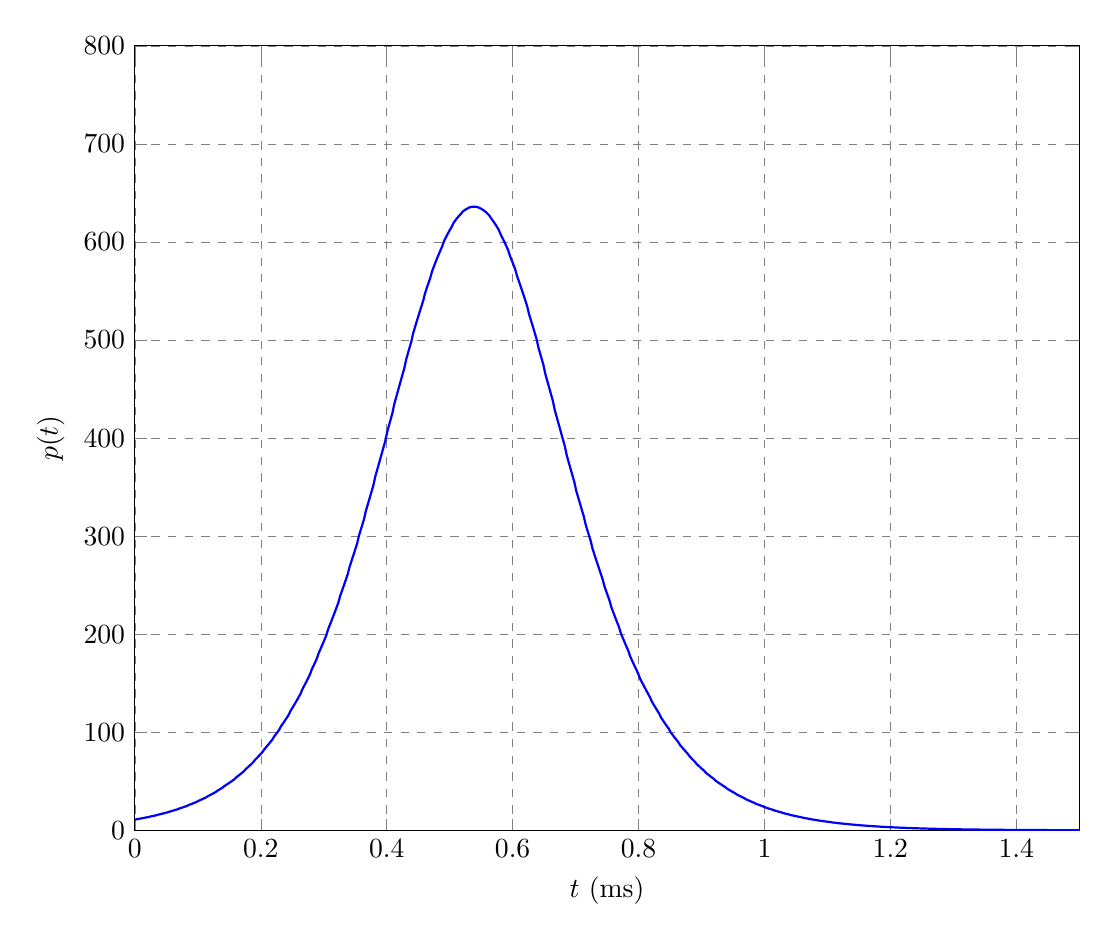
\begin{tikzpicture} \begin{axis}
[scale=1.75, 
 xmin=0, xmax=1.5,
 ymin=0, ymax=800,
 grid=major, 
 major grid style={color=gray,line width=0.2pt, dashed},
 xlabel=$t$ (ms),
 ylabel=$p(t)$,
]

\addplot[line width=0.8pt, color=blue] coordinates {
( 0.000, 11.000 )( 0.004, 11.420 )( 0.008, 11.856 )( 0.011, 12.309 )( 0.015, 12.779 )( 0.019, 13.266 )( 0.023, 13.772 )( 0.026, 14.297 )( 0.030, 14.842 )( 0.034, 15.407 )( 0.037, 15.994 )( 0.041, 16.602 )( 0.045, 17.233 )( 0.049, 17.888 )( 0.053, 18.568 )( 0.056, 19.273 )( 0.060, 20.004 )( 0.064, 20.763 )( 0.068, 21.550 )( 0.071, 22.366 )( 0.075, 23.212 )( 0.079, 24.090 )( 0.083, 25.000 )( 0.086, 25.944 )( 0.090, 26.923 )( 0.094, 27.938 )( 0.098, 28.990 )( 0.101, 30.081 )( 0.105, 31.212 )( 0.109, 32.384 )( 0.113, 33.599 )( 0.116, 34.859 )( 0.120, 36.164 )( 0.124, 37.516 )( 0.128, 38.918 )( 0.131, 40.370 )( 0.135, 41.874 )( 0.139, 43.432 )( 0.142, 45.046 )( 0.146, 46.718 )( 0.150, 48.449 )( 0.154, 50.242 )( 0.158, 52.098 )( 0.161, 54.019 )( 0.165, 56.008 )( 0.169, 58.066 )( 0.173, 60.197 )( 0.176, 62.401 )( 0.180, 64.681 )( 0.184, 67.039 )( 0.188, 69.479 )( 0.191, 72.001 )( 0.195, 74.609 )( 0.199, 77.305 )( 0.203, 80.092 )( 0.206, 82.971 )( 0.210, 85.946 )( 0.214, 89.020 )( 0.218, 92.193 )( 0.221, 95.470 )( 0.225, 98.853 )( 0.229, 102.344 )( 0.232, 105.947 )( 0.236, 109.663 )( 0.240, 113.495 )( 0.244, 117.446 )( 0.247, 121.519 )( 0.251, 125.716 )( 0.255, 130.040 )( 0.259, 134.492 )( 0.263, 139.076 )( 0.266, 143.794 )( 0.270, 148.647 )( 0.274, 153.639 )( 0.278, 158.771 )( 0.281, 164.045 )( 0.285, 169.463 )( 0.289, 175.027 )( 0.292, 180.737 )( 0.296, 186.596 )( 0.300, 192.604 )( 0.304, 198.763 )( 0.307, 205.073 )( 0.311, 211.535 )( 0.315, 218.148 )( 0.319, 224.912 )( 0.323, 231.828 )( 0.326, 238.894 )( 0.330, 246.109 )( 0.334, 253.472 )( 0.338, 260.981 )( 0.341, 268.633 )( 0.345, 276.427 )( 0.349, 284.357 )( 0.353, 292.422 )( 0.356, 300.617 )( 0.360, 308.936 )( 0.364, 317.376 )( 0.367, 325.930 )( 0.371, 334.592 )( 0.375, 343.354 )( 0.379, 352.210 )( 0.382, 361.152 )( 0.386, 370.169 )( 0.390, 379.254 )( 0.394, 388.397 )( 0.398, 397.585 )( 0.401, 406.810 )( 0.405, 416.058 )( 0.409, 425.316 )( 0.412, 434.573 )( 0.416, 443.815 )( 0.420, 453.027 )( 0.424, 462.194 )( 0.428, 471.301 )( 0.431, 480.334 )( 0.435, 489.275 )( 0.439, 498.108 )( 0.442, 506.817 )( 0.446, 515.384 )( 0.450, 523.792 )( 0.454, 532.023 )( 0.458, 540.061 )( 0.461, 547.887 )( 0.465, 555.484 )( 0.469, 562.834 )( 0.472, 569.921 )( 0.476, 576.727 )( 0.480, 583.236 )( 0.484, 589.431 )( 0.488, 595.298 )( 0.491, 600.820 )( 0.495, 605.984 )( 0.499, 610.776 )( 0.503, 615.183 )( 0.506, 619.192 )( 0.510, 622.795 )( 0.514, 625.979 )( 0.518, 628.737 )( 0.521, 631.060 )( 0.525, 632.942 )( 0.529, 634.379 )( 0.532, 635.365 )( 0.536, 635.897 )( 0.540, 635.975 )( 0.544, 635.599 )( 0.547, 634.768 )( 0.551, 633.486 )( 0.555, 631.756 )( 0.559, 629.584 )( 0.563, 626.974 )( 0.566, 623.936 )( 0.570, 620.476 )( 0.574, 616.605 )( 0.578, 612.333 )( 0.581, 607.672 )( 0.585, 602.634 )( 0.589, 597.234 )( 0.593, 591.484 )( 0.596, 585.399 )( 0.600, 578.996 )( 0.604, 572.290 )( 0.607, 565.298 )( 0.611, 558.036 )( 0.615, 550.522 )( 0.619, 542.773 )( 0.623, 534.806 )( 0.626, 526.639 )( 0.630, 518.290 )( 0.634, 509.775 )( 0.638, 501.113 )( 0.641, 492.321 )( 0.645, 483.415 )( 0.649, 474.412 )( 0.652, 465.329 )( 0.656, 456.180 )( 0.660, 446.982 )( 0.664, 437.749 )( 0.667, 428.496 )( 0.671, 419.236 )( 0.675, 409.983 )( 0.679, 400.749 )( 0.683, 391.547 )( 0.686, 382.388 )( 0.690, 373.282 )( 0.694, 364.240 )( 0.698, 355.271 )( 0.701, 346.385 )( 0.705, 337.590 )( 0.709, 328.892 )( 0.713, 320.301 )( 0.716, 311.821 )( 0.720, 303.460 )( 0.724, 295.222 )( 0.727, 287.112 )( 0.731, 279.134 )( 0.735, 271.294 )( 0.739, 263.593 )( 0.743, 256.034 )( 0.746, 248.621 )( 0.750, 241.355 )( 0.754, 234.237 )( 0.757, 227.270 )( 0.761, 220.453 )( 0.765, 213.788 )( 0.769, 207.275 )( 0.772, 200.913 )( 0.776, 194.702 )( 0.780, 188.642 )( 0.784, 182.732 )( 0.787, 176.971 )( 0.791, 171.357 )( 0.795, 165.889 )( 0.799, 160.566 )( 0.802, 155.385 )( 0.806, 150.346 )( 0.810, 145.445 )( 0.814, 140.681 )( 0.818, 136.051 )( 0.821, 131.554 )( 0.825, 127.186 )( 0.829, 122.946 )( 0.833, 118.831 )( 0.836, 114.838 )( 0.840, 110.965 )( 0.844, 107.210 )( 0.848, 103.568 )( 0.851, 100.039 )( 0.855, 96.620 )( 0.859, 93.307 )( 0.863, 90.098 )( 0.866, 86.991 )( 0.870, 83.982 )( 0.874, 81.070 )( 0.878, 78.252 )( 0.881, 75.525 )( 0.885, 72.887 )( 0.889, 70.336 )( 0.892, 67.868 )( 0.896, 65.482 )( 0.900, 63.175 )( 0.904, 60.945 )( 0.907, 58.790 )( 0.911, 56.707 )( 0.915, 54.694 )( 0.919, 52.750 )( 0.922, 50.872 )( 0.926, 49.058 )( 0.930, 47.306 )( 0.934, 45.614 )( 0.938, 43.980 )( 0.941, 42.403 )( 0.945, 40.880 )( 0.949, 39.410 )( 0.953, 37.992 )( 0.956, 36.623 )( 0.960, 35.302 )( 0.964, 34.027 )( 0.968, 32.796 )( 0.971, 31.610 )( 0.975, 30.465 )( 0.979, 29.360 )( 0.983, 28.295 )( 0.986, 27.267 )( 0.990, 26.276 )( 0.994, 25.320 )( 0.998, 24.399 )( 1.001, 23.510 )( 1.005, 22.653 )( 1.009, 21.826 )( 1.013, 21.030 )( 1.016, 20.262 )( 1.020, 19.521 )( 1.024, 18.807 )( 1.028, 18.119 )( 1.031, 17.456 )( 1.035, 16.816 )( 1.039, 16.200 )( 1.042, 15.606 )( 1.046, 15.034 )( 1.050, 14.482 )( 1.054, 13.950 )( 1.058, 13.438 )( 1.061, 12.944 )( 1.065, 12.468 )( 1.069, 12.010 )( 1.072, 11.568 )( 1.076, 11.143 )( 1.080, 10.732 )( 1.084, 10.337 )( 1.087, 9.957 )( 1.091, 9.590 )( 1.095, 9.236 )( 1.099, 8.896 )( 1.103, 8.568 )( 1.106, 8.252 )( 1.110, 7.947 )( 1.114, 7.654 )( 1.117, 7.372 )( 1.121, 7.100 )( 1.125, 6.837 )( 1.129, 6.585 )( 1.133, 6.342 )( 1.136, 6.107 )( 1.140, 5.882 )( 1.144, 5.664 )( 1.148, 5.455 )( 1.151, 5.253 )( 1.155, 5.059 )( 1.159, 4.872 )( 1.163, 4.692 )( 1.166, 4.518 )( 1.170, 4.351 )( 1.174, 4.190 )( 1.178, 4.035 )( 1.181, 3.886 )( 1.185, 3.742 )( 1.189, 3.603 )( 1.192, 3.470 )( 1.196, 3.342 )( 1.200, 3.218 )( 1.204, 3.099 )( 1.208, 2.984 )( 1.211, 2.873 )( 1.215, 2.767 )( 1.219, 2.664 )( 1.223, 2.566 )( 1.226, 2.471 )( 1.230, 2.379 )( 1.234, 2.291 )( 1.237, 2.206 )( 1.241, 2.124 )( 1.245, 2.046 )( 1.249, 1.970 )( 1.252, 1.897 )( 1.256, 1.826 )( 1.260, 1.759 )( 1.264, 1.694 )( 1.268, 1.631 )( 1.271, 1.570 )( 1.275, 1.512 )( 1.279, 1.456 )( 1.282, 1.402 )( 1.286, 1.350 )( 1.290, 1.300 )( 1.294, 1.252 )( 1.298, 1.205 )( 1.301, 1.161 )( 1.305, 1.118 )( 1.309, 1.076 )( 1.312, 1.036 )( 1.316, 0.998 )( 1.320, 0.961 )( 1.324, 0.925 )( 1.328, 0.891 )( 1.331, 0.858 )( 1.335, 0.826 )( 1.339, 0.795 )( 1.343, 0.766 )( 1.346, 0.737 )( 1.350, 0.710 )( 1.354, 0.684 )( 1.358, 0.658 )( 1.361, 0.634 )( 1.365, 0.610 )( 1.369, 0.588 )( 1.373, 0.566 )( 1.376, 0.545 )( 1.380, 0.525 )( 1.384, 0.505 )( 1.387, 0.486 )( 1.391, 0.468 )( 1.395, 0.451 )( 1.399, 0.434 )( 1.403, 0.418 )( 1.406, 0.403 )( 1.410, 0.388 )( 1.414, 0.373 )( 1.418, 0.359 )( 1.421, 0.346 )( 1.425, 0.333 )( 1.429, 0.321 )( 1.433, 0.309 )( 1.436, 0.298 )( 1.440, 0.287 )( 1.444, 0.276 )( 1.448, 0.266 )( 1.451, 0.256 )( 1.455, 0.246 )( 1.459, 0.237 )( 1.462, 0.228 )( 1.466, 0.220 )( 1.470, 0.212 )( 1.474, 0.204 )( 1.477, 0.196 )( 1.481, 0.189 )( 1.485, 0.182 )( 1.489, 0.175 )( 1.492, 0.169 )( 1.496, 0.162 )( 1.500, 0.156 )
};

%\legend{Fuel,Moderator}
\end{axis}
\end{tikzpicture}
\caption{Flux amplitude in a superprompt transient.}
 \label{Fig:kinetics_superpromptTransientFeedback}
\end{center}
\end{figure}

Figure~\ref{Fig:kinetics_superpromptTransientFeedback} depicts an example case for the flux amplitude using the following parameters:
\begin{align}
  \Lambda = 10^{-5} \text{ s}, \quad \rho_1 = 1.1\text{\$}, \quad \gamma = -0.8 \text{ \$/fp-s}. \nonumber
\end{align}
At $t = 0$, the flux amplitude starts at $\tilde{p}_0$ the level after the prompt jump and rises exponentially. 

After about 0.25~ms, feedback effects begin to become important and the reactivity begins to decline. After about 0.5~ms, the flux amplitude reaches its maximum. It is at this point the reactivity falls below prompt supercritical and the flux amplitude declines. Note that this model does not take into account delayed neutron emission. In reality, there is an inventory of delayed neutron precursors that gets produced during the prompt transient that then subsequently decay and produced neutrons. Instead of the flux amplitude falling to zero, it will level off to a higher level than the initial level prior to the transient. This steady level steadily declines as the delayed neutron precursors undergo radioactive decay.

\section{Fission Product Poisons}

Some fission products have large neutron capture cross sections. A handful of these are produced in a significant abundance such that their buildup and presence significantly increases the thermal capture of the fuel, decreasing the reactivity. There are two fission product chains that meet both of these criteria. By far the most important of these are $^{135}$I and $^{135}$Xe, which has a major impact on the operational characteristics of thermal reactors. The other one is $^{149}$Pm and $^{149}$Sm, which has a much smaller, but non-negligible impact on the reactivity. The half lives of these two species are on the order of hours, which introduces a medium timescale reactivity feedback mechanism that must be designed for.

\subsection{Xenon Poisoning}

The fission product $^{135}$I is produced in significant quantities, about 0.063 per fission, either directly or through relatively rapid $\beta^-$ decays of other fission fragments such as $^{135}$Te in its decay chain. $^{135}$I by itself is not particularly noteworthy in terms of its neutron capture cross section, being comparable to other fission products and having a half life of about 6.7~hours, which is not particularly unusual. 

Its immediate decay product $^{135}$Xe, however, has an enormous cross thermal capture section of approximately 2.6~\emph{million} barns, which is by far the highest of any known isotope. $^{135}$Xe is also radioactive, having a half-life of 9.2~hours. The consequence of this abnormally large cross section and high yield is that when a reactor operates, the absorption of the fuel increases, decreasing the reactivity until an equilibrium level is reached from the production from the decay of $^{135}$I and the destruction from either decaying itself or being transmuted to $^{136}$Xe by way of neutron capture. This effect is a bit of nuisance. 

More important is that when a reactor operates at a full power, it produces a large inventory of $^{135}$I that is proportional to the local scalar flux in the fuel. When the reactor shuts down, either intentionally or because of the detection of an abnormal condition, this inventory decays into $^{135}$Xe. Since the reactor is operating, there are not a significant number of neutron captures to remove them and the population of  $^{135}$Xe grows over the time scale of several hours to a much higher level than would be possible if the reactor were operating. The amount of $^{135}$Xe is often so large that it literally becomes impossible to restart the reactor for a period of time until the $^{135}$Xe decays to a sufficient amount. This condition is called \emph{poisoning out}. (In principle it is possible to design around this by including sufficient excess reactivity, but for power reactors on low-enriched uranium, it is impractical to do so.)

So when a reactor shuts down unintentionally, the operators typically have a few hours to address any problems and restart the reactor before a sufficient amount of $^{135}$Xe builds up. If this cannot be done, the operators must wait several hours (on the order of a day) for the poison to naturally decay away.

We can describe the density of $^{135}$I and $^{135}$Xe using radioactive decay equations by $I(t)$ and $X(t)$ respectively. For $^{135}$I, this is
\begin{align}
  \frac{dI}{dt} = 
  \underbrace{\gamma_I \Sigma_f \phi(t)}_{\parbox{2.5cm}{\scriptsize rate $^{135}$I is produced from fission, either directly or from decay of parent nuclei}} 
  - \underbrace{\lambda_I I(t)}_{\parbox{2cm}{\scriptsize rate $^{135}$I is removed by radioactive decay.}}  ,
\end{align}
and for $^{135}$Xe, we have
\begin{align}
  \frac{dX}{dt} = 
  \underbrace{\gamma_X \Sigma_f \phi(t)}_{\parbox{2.5cm}{\scriptsize rate $^{135}$Xe is produced directly from fission}}
  + \underbrace{\lambda_I I(t)}_{\parbox{2cm}{\scriptsize rate $^{135}$Xe is produced by decay of $^{135}$I}}  
  - \underbrace{\lambda_X X(t)}_{\parbox{2cm}{\scriptsize rate $^{135}$Xe is removed by radioactive decay.}}  
  - \underbrace{\sigma_a^X \phi(t) X(t)}_{\parbox{2.5cm}{\scriptsize rate $^{135}$Xe is removed by neutron capture.}}.
\end{align}
Typical values for these constants for $^{235}$U fission are as follows:
\begin{align}
   \gamma_I = 0.0628, \ \gamma_X = 0.00257, \ \lambda_I = 0.1035 \text{ hr$^{-1}$}, \ \lambda_X = 0.0753 \text{ hr$^{-1}$}, \  \sigma_a^X = 2.6 \text{ Mb}. \nonumber
\end{align}
Different fissionable isotopes have different yields that need to be looked up.

A few comments. First, we neglected the removal of $^{135}$I by neutron capture. A realistic calculation should include this, but in practice the contribution is small compared to decay. Second, $\gamma_I$ is the \emph{cumulative} fission product yield, which includes both direct production from fission and decays from all of its parent nuclei, whereas $\gamma_X$ is the \emph{independent} yield that only includes direct production from fission. Third, these are local to a particular region since $\phi$ depends on position throughout the reactor and we need to solve a decay equation for each spatial zone to get the local concentrations of the fission product poisons. Finally, care needs to be taken to use consistent units. The scalar flux typically has units of per area in cm$^2$, whereas cross sections have units of barns with 1 b $ = 10^{-24}$~cm$^2$.

If we assume $\phi(t) = \phi_0$ is constant in time, then solving these equations is straightforward, just a bit tedious of algebra. The solutions are
\begin{subequations}
\begin{align}
  I(t) &= \frac{ \gamma_I \Sigma_f \phi_0 }{ \lambda_I } \left( 1 - e^{-\lambda_I t } \right), \\
  X(t) 
  &= \frac{ ( \gamma_I + \gamma_X ) \Sigma_f \phi_0 }{ \lambda_X + \sigma_a^X \phi_0 } \left[ 1 - \exp \left( -\left( \lambda_X + \sigma_a^X \phi_0 \right) t \right) \right] \nonumber \\
  &+ \frac{ \gamma_I \Sigma_f \phi_0 }{ \lambda_X - \lambda_I + \sigma_a^X \phi_0 } \left[  \exp \left( -\left( \lambda_X + \sigma_a^X \phi_0 \right) t \right) - \exp \left( -\lambda_I t \right) \right] .
\end{align}
\end{subequations}

In practice, however, the $^{135}$Xe concentration impacts the local scalar flux and vice versa, so we need to use some numerical technique to solve the rate equations and the neutron transport or diffusion equation.  One approach is to use a standard time-stepping or forward Euler approach. This requires an impractical number of time steps, so we use a more advanced scheme called the predictor-corrector method. We detail this in Sec.~\ref{Sec:kinetics_fuelDepletionEquations}, since it applies to generic isotopic depletion problems.

Regarding the fission product poisons specifically, we are most interested in the \emph{equilibrium} concentrations after the reactor has been operating for some time. This can be solved given a flux level $\phi_0$ (proportional to reactor power) by either letting $t \rightarrow \infty$ in the above equation or more simply by setting the time derivatives in the differential equations to zero and solving the algebraic equations. The equilibrium $^{135}$I and $^{135}$Xe concentrations are
\begin{subequations} \label{Eq:kinetics_iodineXenonEquilibrium}
\begin{align}
  I_\infty &=  \frac{ \gamma_I \Sigma_f \phi_0 }{ \lambda_I } , \\
  X_\infty &=  \frac{ ( \gamma_I + \gamma_X ) \Sigma_f \phi_0 }{ \lambda_X + \sigma_a^X \phi_0  } . \label{Eq:kinetics_xenonEquilibrium}
\end{align}
\end{subequations}

For a typical power reactor, the average thermal scalar flux at hot-full power is on the order of $10^{14}$~cm$^{-2}\cdot$s$^{-1}$. (Research and isotope production reactors can have even higher fluxes in excess of $10^{15}$~cm$^{-2}\cdot$s$^{-1}$.) This is large enough such that the $\phi_0$ terms dominate and
\begin{align}
  X_\infty \approx \frac{ ( \gamma_I + \gamma_X ) \Sigma_f  }{ \sigma_a^X } , \quad   \phi_0 \gg \frac{\lambda_X}{\sigma_a^X} . 
\end{align}
This means that as the scalar flux and reactor power rises, the $^{135}$Xe concentration tends to saturate and does not appreciably increase with power level past a certain point and just depend on the material and nuclear properties. This is rather convenient as it makes it possible to estimate the negative reactivity insertion from the buildup of $^{135}$Xe.

One complication here is that $\phi_0$ is not a constant throughout the reactor core and may vary with position. Rather we are given the \emph{average} scalar flux $\overline{\phi}$ in the fuel, which is proportional to the reactor power. Because of this dependence and the fact that the local scalar flux depends on the $^{135}$Xe concentration and vice versa, we need to iterate to find the local values. 

The process is to solve a neutron transport or diffusion problem to find the scalar fluxes in the fuel normalized to the power, which is proportional to $\overline{\phi}$. We then use Eq.~\eqref{Eq:kinetics_iodineXenonEquilibrium} to guess the $^{135}$I and $^{135}$Xe concentrations at each local position. We then use these fission product concentrations in another neutron transport or diffusion solve to compute updated scalar fluxes that are again renormalized. We then use these scalar fluxes to update the poison concentrations. The process repeats until convergence. Fortunately, because the local effect on the reactivity tends to saturate for high scalar fluxes, this iteration tends to be quite stable.

We can estimate the effect on the reactivity using one-speed neutron diffusion with perturbation theory. For an \emph{infinite medium} the estimated change in reactivity for going from no $^{135}$Xe to the equilibrium state is
\begin{align}
  (\Delta \rho)_\text{Xe} \approx -\frac{ \Delta \Sigma_a }{ \nu \Sigma_f } = -\frac{ \sigma_a^X X_\infty }{ \nu \Sigma_f } =  -\frac{ \sigma_a^X ( \gamma_I + \gamma_X ) \Sigma_f \phi_0 }{ \nu \Sigma_f ( \lambda_X + \sigma_a^X \phi_0 )  } = -\frac{ \sigma_a^X ( \gamma_I + \gamma_X ) \phi_0 }{ \nu ( \lambda_X + \sigma_a^X \phi_0 )  }
\end{align}
At hot-full power conditions for a typical power reactor, $\phi_0$ is sufficiently large to we can eliminate the $\lambda_X$ term in the denominator and approximate the change in reactivity as
\begin{align}
  (\Delta \rho)_\text{Xe} \approx  -\frac{ ( \gamma_I + \gamma_X ) }{ \nu  } , \quad   \phi_0 \gg \frac{\lambda_X}{\sigma_a^X} .
\end{align}
For $^{235}$U this is approximately $-0.027$ or about $-4$\$ depending on the effective delayed neutron fraction of the system. Of course, there are a few assumptions with obtaining this estimate and the actual value may be different for a real system, but the ballpark is that a reactor needs an few dollars of excess reactivity to compensate for the buildup of $^{135}$Xe during full-power operation.

The equilibrium $^{135}$I concentration on the other hand, increases proportionally to the scalar flux $\phi_0$ and does not saturate at any practically achievable flux level. This means the higher the operating scalar flux, the larger the inventory of $^{135}$I at shutdown is, and the concentration of $^{135}$Xe that builds up will be higher. We can solve for the $^{135}$I and $^{135}$Xe concentrations post shutdown by solving the rate equations with $\phi_0 = 0$ using $I_\infty$ and $X_\infty$ as initial conditions. The solutions are
\begin{subequations}
\begin{align}
  I(t) &= I_\infty e^{-\lambda_I t}, \\
  X(t) &= X_\infty e^{-\lambda_X t} + \frac{ \lambda_I I_\infty }{ \lambda_I - \lambda_X } \left( e^{-\lambda_X t} - e^{-\lambda_I t} \right) .
\end{align}
\end{subequations}
Because $I_\infty$ is proportional to the operating scalar flux $\phi_0$, the second term in the post-shutdown $^{135}$Xe concentration equation tends to be large when $\phi_0$ is large. This second term accounts for the buildup and subsequent decay of $^{135}$Xe from the decay of $^{135}$I after shutdown.

We can show that if
\begin{align}
  \phi_0 < \frac{ \gamma_X \lambda_X }{ \gamma_I \sigma_a^X },
\end{align}
then there will be no buildup of $^{135}$Xe, since the maximal value is at shutdown. This ratio is about $4 \times 10^{11}$~cm$^{-2}\cdot$s$^{-1}$ for $^{235}$U fission, which is much lower than for a power reactor. So in practice, there will be a buildup of $^{135}$Xe where the maximum time is
\begin{align}
  t_\text{max} = \frac{1}{\lambda_I - \lambda_X} \ln \left[ \dfrac{ \lambda_I / \lambda_X }{ 1 + \dfrac{\lambda_X}{\lambda_I} \left( \dfrac{\lambda_I}{\lambda_X} - 1 \right) \dfrac{X_\infty}{I_\infty} } \right] .
\end{align}
For typical power reactors, we have
\begin{align}
  t_\text{max} \approx \frac{1}{\lambda_I - \lambda_X} \ln \left( \frac{\lambda_I}{\lambda_X} \right) = 11.6 \text{ hr}, \quad  \phi_0 \gg \frac{\lambda_X}{\sigma_a^X} .
\end{align}
The decay of $^{135}$Xe proceeds and depending on the operating flux level and the amount of excess reactivity available, the operators need to wait several hours beyond this before the reactor can be restarted. A typical value for the total poison out time is again, on the order of a day.

\subsection{Samarium Poisoning}

$^{135}$Xe is by far the dominant fission product poison. Of the remaining, there is one one other that is both produced in sufficient quantities and has a high enough capture cross section to be individually analyzed. This is $^{149}$Sm, which is a $\beta^-$ decay product from the chain starting with $^{149}$Ba decaying through $^{149}$Pm, which has a relatively long half life, and finally to the fission product poison itself. Most of the direct production comes from $^{149}$Ce or $^{149}$Pr, but these decay rapidly. 

As with the iodine-xenon chain, we often lump the production into the $^{149}$Pm fission product poison precursor as $^{149}$Nd and all its parent nuclides have a relatively short half lives--$^{149}$Nd decays in about 1.7 hours versus 53 hours for $^{149}$Pm. The major difference between $^{149}$Sm and $^{135}$Xe is that the former is stable, which makes the dynamics different and simpler.

We denote the $^{149}$Pm and $^{149}$Sm concentrations as $P(t)$ and $S(t)$ respectively. They satisfy the following rate equations:
\begin{align}
  \frac{dP}{dt} &= \gamma_P \Sigma_f \phi(t) - \lambda_P P(t), \\
  \frac{dS}{dt} &= \lambda_P P(t) - \sigma_a^S \phi(t) P(t).
\end{align}
As with $^{135}$I, the neutron capture of $^{149}$Pm is small enough that we can neglect it. One difference is that the direct production of $^{149}$Sm from fission is negligible, having an estimated direct yield of about $1.7 \times 10^{-12}$, so we exclude that term. Typical values for these constants with $^{235}$U fission are
\begin{align}
  \gamma_P = 0.0108, \ \lambda_P = 0.01306 \text{ hr$^{-1}$}, \ \sigma_a^S = 40.51 \text{ kb}. \nonumber
\end{align}

Again, assuming a constant scalar flux $\phi_0$, we can solve these rate equations and arrive at the equilibrium concentrations. These are
\begin{subequations}
\begin{align}
  P_\infty &= \frac{ \gamma_P \Sigma_f \phi_0 }{ \lambda_P } , \\
  S_\infty &= \frac{ \gamma_P \Sigma_f }{ \sigma_a^S } .
\end{align}
\end{subequations}
The reactivity effect of equilibrium ${149}$Sm can be similarly computed for a one-speed, infinite homogeneous mixture:
\begin{align}
  ( \Delta \rho )_\text{Sm} = -\frac{\sigma_a^S S_\infty}{\nu\Sigma_f} = -\frac{\Delta\Sigma_a}{\nu\Sigma_f} = -\frac{ \gamma_P \Sigma_f }{ \nu \Sigma_f \sigma_a^S } = -\frac{\gamma_P}{\nu} = -4.46 \times 10^{-3}.
\end{align}
Assuming an effective delayed neutron fraction of 0.007, this gives a ballpark estimate of $-0.64$\$ of reactivity. This implies that the reactivity effect for equilibrium $^{135}$Xe is on the order of six times greater than for equilibrium $^{149}$Sm.

The more important behavior for both $^{135}$Xe and $^{149}$Sm are post shutdown. In both cases, there is an inventory of the fission poison precursor built up that is proportional to the operating scalar flux that leads to a negative reactivity insertion following shutdown. Unlike $^{135}$Xe, the isotope $^{149}$Sm is stable, so the negative reactivity insertion is ``permanent'' in that it lasts until the reactor is turned back on and the $^{149}$Sm is burned away. So one cannot wait out the $^{149}$Sm transient unlike with $^{135}$Xe. Thankfully, the negative reactivity insertion is much smaller and we can much more easily manage around it. (It is theoretically possible to poison out on $^{149}$Sm, perhaps near the end of a fueling cycle, and this would require adding new fuel or doing a reshuffling.)

To analyze this, we can easily derive the post shutdown poison concentration as
\begin{align}
  S(t) = S_\infty + P_\infty ( 1 - e^{-\lambda_P t} ) .
\end{align}
This implies in the long run the entire $^{149}$Pm inventory decays into $^{119}$Sm and stays there. The negative reactivity insertion after a prolonged shutdown is
\begin{align}
  \Delta \rho = -\frac{\gamma_P}{\nu} \left( 1 + \frac{\sigma_a^S \phi_0 }{\lambda_P} \right) .
\end{align}
For a typical power reactor flux level of $10^{14}$~cm$^{-2}\cdot$s$^{-1}$ with $^{235}$U fission, this equates to a negative reactivity insertion of about $-0.0095$ or about $-1.35$\$ using the same effective delayed fraction of 0.007. This is large enough that it cannot be ignored, but it is not nearly as much a concern as for $^{135}$Xe.

Beyond $^{149}$Sm, there are just not any other fission product poisons with both a high enough yield and cross section. While modern analyses treat each fission product explicitly, older numerical techniques or simplified analyses use a single permanent lumped fission product poison that is assumed to be produced by any fission not creating $^{135}$I, $^{135}$Xe, or $^{149}$Pm. This lumped fission product poison typically has a capture cross section of about 50~b and slowly builds into the fuel. When a neutron is captured by this permanent poison, we assume that it simply converts into another fission product poison that is equivalent.

\subsection{Xenon Spatial Oscillations}

There is an important consideration related to $^{135}$Xe in large thermal reactors, which account for most operating power reactors. When a reactor is large, we say that it is \emph{neutronically decoupled} in the sense that a perturbation in one part of the reactor does not directly influence the neutrons in another part. The typical value for such a system is in excess of 30 neutron migration lengths, which again is most commercial reactors. In this case, we can develop a large concentration of $^{135}$Xe that migrates periodically throughout the reactor core, which locally depresses the flux.

To understand how this happens, suppose in one part of the reactor the neutron flux is higher compared to other parts of the reactor. This occurs naturally because of heterogeneities from moderator density differences from temperature or control rod placement axially. In this region of high flux, the local inventory of $^{135}$Xe will be burned up, driving a further increase in the flux level.

If the reactor is to held at a constant power, which is the case for standard operations, this local increase in flux must be offset by a decrease elsewhere, leading to a spatial tilt in the flux. Simultaneously, the other side of the reactor that had a low flux produces less $^{135}$I and therefore the inventory of $^{135}$Xe on that side depletes from radioactive decay. Eventually, the inventory of $^{135}$Xe on the high flux side gets sufficiently depleted such that the flux stops increasing, but the increased fission produces more $^{135}$I that then, in a matter of hours, decays to $^{135}$Xe. This buildup of $^{135}$Xe then decreases the power locally, and to hold the power constant, the flux on the other side must increase, reversing the tilt from one side to the other and the process repeats, but on the opposite sides. This causes an oscillation to form between the $^{135}$Xe and scalar flux between each side of the reactor that has a period on the order of 15-30 hours. 

The problem with having such an oscillation is that we normally desire the scalar flux to be spatially flat. The reason for this is the operational fuel temperature limits are driven by the local peak power and not the average, i.e., if the fuel exceeds its safe operating range anywhere in the reactor, it can lead to a fuel failure or exceed critical heat flux limits. Having such an oscillation leads to increased peaking (a local hot spot) and limits the operating power of the reactor. 

As such, we design a reactor to minimize the formation and impact of these spatial oscillations. Should they form, it is possible to move control rods into the reactor partially to suppress them. These motions are fairly complex and need to be built into the operational procedures.

\section{Reactor Fuel Cycles}

Over time the inventory of fissionable nuclides in the reactor depletes. When neutrons cause fission, the fuel isotope is split into two fragments. These fragments are usually radioactive and undergo decay, which generates further heat. While this thermal energy from repeated radioactive decay needs to be removed continuously for years to prevent the fuel from overheating, it is not sufficient to drive an energy conversion cycle. Therefore, these radioactive fragments are a waste byproduct of fission that must be managed. From the reactor's perspective, each fission means one less fissionable nuclide and there is a reduction in the total amount of excess reactivity in the reactor. 

The buildup of fission product poisons and the associated oscillations is on the timescale of hours and days. On the longer timescale of weeks or months, the depletion of the fuel via fission or burnable absorbers via capture must be considered. On one hand. the depletion of fuel decreases the reactivity because there is less fissionable material. On the other, the depletion of the burnable absorbers increases the reactivity because once they capture neutrons they lose their ability to capture further neutrons. Additionally, the fuel of power reactors consists primarily $^{238}$U, which is responsible for much of the absorption of neutrons. This neutron capture reaction produces $^{239}$U, which rapidly decays to $^{239}$Np, and after about 2.4 days, decays into $^{239}$Pu, which is itself fissile. Furthermore, this inventory of $^{239}$Pu captures neutrons to make $^{240}$Pu and then can capture another to make $^{241}$Pu, and so on. We refer to this as the conversion of fertile isotopes and is a long-term increase in reactivity (so long as we do not run out of fertile material.)

On balance, a typical thermal reactor has enough fuel and excess reactivity to sustain operations for about 18-24 months before new fuel needs to be cycled into the reactor. In other words the depletion of fuel dominates the production of fissile isotopes from conversion. At the end of a typical reactor cycle, about a third of the power comes from various Pu isotopes.

\subsection{Overall Nuclear Fuel Cycle}

\begin{figure}[tb!]
\begin{center}
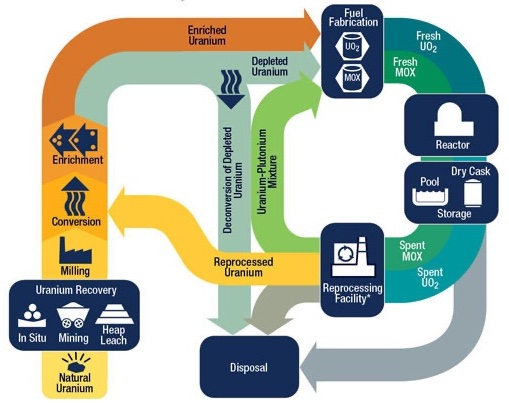
\includegraphics[width=0.8\textwidth]{./Figures/NRCFuelCycle.jpg}
\caption{Illustration of the nuclear fuel cycle (US Nuclear Regulatory Commission)}
\label{Fig:kinetics_nuclearFuelCycle}
\end{center}
\end{figure}

Before going into the analysis of the reactor, it is helpful to zoom out to the big picture of how the entire nuclear fuel cycle functions. This is depicted in Fig.~\ref{Fig:kinetics_nuclearFuelCycle}.

Before going into details, there are two primary types of fuel cycles in use. The US uses a once-through fuel cycle where fuel is put into a reactor, burned, and then disposed of as waste. France and Japan, on the other hand, perform fuel recycling, extracting the plutonium and blending it with uranium fuel to make mixed-oxide or MOX fuel assemblies that are then put back into reactors for additional burnup. 

The advantages of recycling is that it has a greater resource utilization and reduces the quantity of spent nuclear fuel that must be managed. The disadvantage is this comes at an increased cost, as mining uranium is inexpensive. Second, there is an increased risk of diversion of weapons usable materials. While reactor grade plutonium contains too much $^{240}$Pu to be an ideal nuclear explosive and is not the most attractive route for a nation state to pursue, it is nonetheless possible to use it for that purpose. This increased risk must be offset by increased costs to minimize the possibilities of such fuel diversions.

The once-through nuclear fuel cycle consists of the following major steps:
\begin{enumerate}
  \item Mining -- uranium is obtained by extracting it from ores underground resources. Like all mining, this is a polluting industry and is arguably the most environmentally damaging part of the nuclear fuel cycle. The argument in favor is because of the energy density of nuclear fuels, we require less mining than other energy sources.
  \item Milling -- the raw uranium ore must be extracted and comes in the composition of U$_3$O$_8$, which is sometimes called yellowcake. 
  \item Conversion -- in the US, fuel must be enriched and U$_3$O$_8$ is not a chemical form that permits this. We convert it into UF$_6$, which readily enters a gaseous phase.
  \item Enrichment -- the gaseous UF$_6$ is put into fast moving centrifuges. Because of the small mass differential between $^{235}$U and $^{238}$ the centrifugal forces preferentially push one isotope out more than other. The stock is moved through a series of such centrifuges until a desired enrichment (usually a few percent) is reached.
  \item Fuel Fabrication -- the enriched UF$_6$ is converted into ceramic UO$_2$ and sintered into pellets and sealed into fuel cladding tubes. These fuel rods are then put into bundles or assembles that are delivered to a power plant.
  \item Reactor -- the fuel is put into the reactor and is used to cause fission, producing thermal and then electrical energy. A typical fuel assembly resides in the reactor between 3-6 years.
  \item Onsite Storage -- once the fuel is sufficiently depleted it is moved out of the reactor for storage. Because of the large inventory of fission products, the fuel continues to generate a large amount of heat because of radioactive decay that must be removed. This is done by placing them into a spent fuel pool where the fuel assembly resides for several years. Once the radioactive inventory has decreased enough, the fuel is moved out of the pool and placed in dry casks that are cooled with air.
  \item Long-term Repository -- while not yet in operation, the plan in the US is to move the fuel in the spent fuel casks into a long-term or permanent repository for final disposition.
\end{enumerate}
 
In a fuel-recycle scenario, sometime after the fuel is removed from the reactor, it is sent to a reprocessing facility where it is chemically dissolved and separated. The plutonium is extracted and then mixed with uranium to create fuel with enough reactivity to go back into a reactor. The recycling process produces waste that must similarly be disposed of, but the volume and radiotoxicity is much less. 

More advanced fuel cycles are currently being investigated that make use of fast reactors that are capable of burning up the fissionable (but not fissile) actinides with long half lives that account for much of the radiotoxicity on the 1,000 to 100,000 year timeframe. While the technology is theoretically in place, it has yet to be demonstrated in an economically competitive manner.

\subsection{Fuel Burnup}

Zooming back into the reactor eventually, the fuel becomes too depleted to effectively sustain a chain reaction and must be removed from the reactor. This can be mitigated by reshuffling the fuel and mixing it with fresh fuel assemblies, but there are still limits. The limiting factor is not the availability of fuel per se, but rather the fuel experiences steady damage from the energetic fission fragments. Additionally, the buildup of these fragments changes the chemistry, leading to corrosive chemical interactions with the cladding. Also, some of the fission products are gases and these fill the sealed fuel-cladding tube and lead to an increase in internal pressure. As the fuel continues to burn up, its structural integrity diminishes and the probability of fuel failure increases with time. Therefore, fuel inventory concerns aside, it is necessary to remove the fuel from the reactor after a few years lest the fuel rods begin to fail and leak fission products into the coolant.

We quantify the fuel exposure to neutrons with a quantity called \emph{burnup}, which is defined as
\begin{align}
  B = \frac{\text{energy released from fission}}{\text{mass of the fissionable material}} .
\end{align}
Typically we express the energy in units of GWd (GigaWatt days), based on the thermal (not electrical) power of the reactor, and the units of mass as MTU, metric tons of uranium (excluding the mass of oxygen in the conventional UO$_2$ fuel). If different fissionable materials are used, then the mass needs to adjusted accordingly and sometimes the denominator is quoted as mass of heavy metal. Further, the mass of fissionable material typically includes all isotopes, not just, for example, the fissile $^{235}$U.

Typical end-of-life burnups for conventional UO$_2$ fuel is between 30 to 40 GWd/MTU. In recent years, there has been considerable effort to developing fuel capable of handling higher burnup, up to around 60 GWd/MTU, which means they can stay in the reactor longer and more energy can be extracted per unit mass. Advanced reactors such as gas-cooled variants use spherical TRISO fuel kernels that are capable of even higher fuel burnups.

\subsection{Conversion Ratio}

As mentioned, some of the fertile $^{238}$U in a reactor is converted into fissile plutonium isotopes. In a conventional reactor, the depletion of $^{235}$U cannot keep up with the creation of plutonium. However, it is possible to create more fuel than is burned in a \emph{breeder reactor}. For thermal reactors, we use a thorium-based cycle where the fertile $^{232}$Th captures neutrons and produces (after a couple $\beta^-$ decays) fissile $^{233}$U, which is the actual fuel. In fast reactors, we typically convert $^{238}$U into Pu isotopes in an external blanket that can then be extracted, chemically separated, and used to make more fuel for other reactors. In the early days of nuclear power, the known resources of uranium was thought to be much more limited than it actually is. Today, there is a large supply of economically mineable uranium resources such that the resource question is far less of an short or medium term concern. That said, there is still interest in thorium cycles or fast reactors, but these are driven by other factors rather than long-term uranium resources.

Regardless of whether the intent is to breed new fuel, some will be produced and this quantity is called the \emph{conversion ratio}. This is
\begin{align}
  C = \frac{\text{production rate of fissile atoms}}{\text{consumption rate of fissile atoms}} .
\end{align}
In a conventional reactor, the conversion ratio is less than one, i.e., the fuel is burned faster than it is produced. For a typical thermal power reactor, this conversion ratio is on the order of 0.5 to 0.6. In a breeder reactor, the conversion ratio is greater than one and is then usually called the \emph{breeding ratio}.

\subsection{Fuel Depletion Equations} \label{Sec:kinetics_fuelDepletionEquations}

Analyzing the depletion of the reactor is actually a very complicated process. Modern methods typically consider every reaction pathway and fission product individually, considering their radioactive decay. This is done by solving the rate equations including depletion and production, which is a series of first-order ordinary differential equations in each spatial region that depends on the local scalar flux $\phi(\pos,t)$. 

The general form of a rate equation in a reactor for isotope $i$ with concentration $N_i$ is
\begin{align}
  \frac{dN_i}{dt} &= 
  \underbrace{\sum_j \lambda_{ji} N_j(t) }_{\parbox{2.25cm}{\scriptsize rate isotope $i$ is produced from radioactive decay of all isotopes $j$}}
  + \underbrace{\sum_j \gamma_{ji} \sigma_{f,j} \phi(t) N_j(t)}_{\parbox{3.5cm}{\scriptsize rate isotope $i$ is produced from fission from all fissionable isotopes $j$}}
  + \underbrace{\sum_j \sigma_{ji} \phi(t) N_j(t)}_{\parbox{2.75cm}{\scriptsize rate isotope $i$ is produced from all non-fission nuclear reactions with isotopes $j$}} \nonumber \\
  &- \underbrace{\sum_x \sigma_{x,i} \phi(t) N_i(t)}_{\parbox{3cm}{\scriptsize rate isotope $i$ is removed because of all nuclear reactions $x$}}
  - \underbrace{\lambda_i N_i(t) }_{\parbox{1.75cm}{\scriptsize rate isotope $i$ is removed by radioactive decay}}.
\end{align}
Here
\begin{align}
  \lambda_{ji} &= \text{decay constant for isotope $j$ decaying to isotope $i$},  \nonumber \\
  \gamma_{ji}  &= \text{fission product yield for isotope $i$ from fissionable nucleus $j$}, \nonumber \\
  \sigma_{ji}  &= \text{reaction cross section for conversion from isotope $j$ into $i$}, \nonumber \\
  \sigma_{x,i} &= \text{cross section for reaction $x$ of isotope $i$}, \nonumber \\
  \lambda_i    &= \text{decay constant for isotope $i$ (for all decays)}. \nonumber 
\end{align}
An equation is written down for each isotope $i$. These equations can then be formed into a linear system as
\begin{align}
  \frac{d\mathbf{N}}{dt} = \mathbf{A}(t) \mathbf{N}(t) ,
\end{align}
where the coefficient matrix $\mathbf{A}$ depends on both the nuclear data and the local scalar flux $\phi(t)$, which carries the time dependence of the matrix. 

If we assume that the scalar flux is constant over some time interval, i.e., a time step in a calculation $t_i \le t < t_{i+1}$, then this system has a solution as the matrix exponential,
\begin{align}
  \mathbf{N}(t) = \exp\left[ (t-t_i) \mathbf{A} \right] \mathbf{N}(t_i) , \quad t_i \le t < t_{i+1} ,
\end{align}
where $\mathbf{N}(t_i)$ is a known initial condition at $t = t_i$, the beginning of the interval.

The complication that arises is similar to that of the fission product poisons in that the changes in local isotopics leads to a change in the local flux. This means that the depletion equations are non-linear and need to be solved numerically on a time grid that is fine enough to capture the temporal changes of the isotopic concentrations. 

The typical numerical scheme used is called the \emph{predictor-corrector method}. The idea is to break the reactor fueling cycle into a series of time steps that are sufficiently small to capture any changes in the reactor conditions. Typically, this means we need a relatively short time step or two to account for the buildup to the equilibrium states of the fission product poisons $^{135}$Xe and $^{149}$Sm every time the reactor changes its power level. Then, we need to take time steps of on the order of a few weeks to capture slower, long term fuel depletion and fertile conversion effects.

Suppose the isotopic compositions are known at the beginning of time step $t_i$ and given in a vector $\mathbf{N}(t_i)$ . We can then solve the neutron transport or diffusion equations using these componsitions with some numerical scheme to get the consistent scalar fluxes. We call these $\phi_1(t_i)$.

We then plug the scalar flux $\phi_1(t_i)$ into the system of rate equations and solve them at each position in the reactor to arrive at a \emph{prediction} of the new isotopic composition vector $\hat{\mathbf{N}}(t_i)$. We could use this prediction as the new isotopic compositions $\mathbf{N}(t_{i+1})$, but it turns out doing this, wile simple, would require taking very large time steps.

Instead, we use this new vector as input into the neutron transport and diffusion equation and solve for an updated scalar flux using the new compositions that we call $\phi_2(\pos,t_i)$. We then go back and compute a \emph{corrected} isotopic composition by using the average of the scalar fluxes,
\begin{align}
  \phi(t_i) = \frac{ \phi_1(t_i) + \phi_2(t_i) }{ 2 } ,
\end{align}
as the scalar flux to compute $\mathbf{N}(t_{i+1})$. We then use this as the initial condition of for the next time step. Because the core composition has changed, we then need to perform a criticality search after each time step based on changing control rod heights or soluble boron concentrations.

Note again that these equations must be solved for all locations in the reactor, so it can become a rather computationally taxing task for a large reactor with numerous fuel pins. Using the predictor-corrector method significantly improves the accuracy of the depletion solve over forward Euler and allows for taking much larger time steps than would be possible otherwise. More sophisticated methods exist, and finding better depletion solver techniques that balance accuracy versus computational costs remains an open area of study.

One thing worth mentioning is that the coefficients in the matrix $\mathbf{A}$ span several orders of magnitude. This implies we have phenomena that occur on timescales ranging from milliseconds to millions of years. It turns out that evaluating the matrix exponential is actually difficult in this case because of numerical precision issues. While this problem has not completely gone away, the last few decades have seen advances in numerical solution techniques capable of handing what we term stiff systems of differential equations, and the issue is far less acute than it used to be.

\subsection{Estimation of Fuel Cycle Length}

The depletion equations can be solved using numerical schemes to determine the fuel cycle length. Normally, the cycle ends when the fuel inventory has been depleted to the point where there is no remaining excess reactivity to make the reactor critical.

We can perform a simple analysis assuming a one-speed, infinite homogeneous medium to illustrate the general considerations, even though such a model is mostly of pedagogical use. We assume that the reactor is operated at a constant power (not a constant flux), which implies that
\begin{align}
  \Sigma_a^F(t) \phi(t) = \Sigma_a^F(0) \phi(0) , \label{Eq:kinetics_simplifiedBurnup_constantPowerFuelXS}
\end{align}
where $\Sigma_a^F(0)$ is the initial fuel loading and $\phi(0)$ is the initial flux level. This implies that the flux must change in time, specifically increasing to offset fuel depletion.

To solve for $\phi(t)$, we write s simple rate equation for the depletion of the fuel,
\begin{align}
  \frac{dN^F}{dt} = -\sigma_a^F N^F(t) \phi(t) = -\sigma_a^F N^F(0) \phi(0) .
\end{align}
Here we used the fact that $\Sigma_a^F \phi$ is constant over the cycle. (We also neglect the radioactive decay of the fuel, which, while not strictly true, is a reasonable assumption since the half life of any practical reactor fuel is going to be much greater than the cycle length.) Since the right-hand side is constant, we can simply integrate this to obtain the fuel atomic density as a function of time,
\begin{align}
  N^F(t) = N^F(0) -\sigma_a^F N^F(0) \phi(0) t = N^F(0) \left[ 1 - \sigma_a^F \phi(0) t \right] .
\end{align}
Multiplying the extreme left and right hand side by $\sigma_a^F$, we get the macroscopic fuel cross section as a function of time,
\begin{align}
  \Sigma_a^F(t) = \Sigma_a^F(0) \left[ 1 - \sigma_a^F \phi(0) t \right] . \label{Eq:kinetics_simplifiedBurnup_fuelAbsorptionXS_time}
\end{align}

We then substitute this into Eq.~\eqref{Eq:kinetics_simplifiedBurnup_constantPowerFuelXS} to obtain the relationship
\begin{align}
  \Sigma_a^F(0) \left[ 1 - \sigma_a^F \phi(0) t \right] \phi(t) = \Sigma_a^F(0) \phi(0) . \nonumber
\end{align}
We can then easily solve this for the scalar flux as a function of time,
\begin{align}
  \phi(t) = \frac{\phi(0)}{ 1 - \sigma_a^F \phi(0) t } . \label{Eq:kinetics_simplifiedBurnup_scalarFlux_time}
\end{align}
We refer to this as the flux history of the reactor needed to ensure a constant power.

For a single thermal energy group, we can write the effective multiplication factor $k$ as the product of the thermal fission factor $\eta = \nu\Sigma_f^F/\Sigma_a^F$ and the thermal utilization factor $f = \Sigma_a^F/\Sigma_a$. Here the absorption cross section $\Sigma_a$ includes components from the fuel $\Sigma_a^F$, moderator $\Sigma_a^M$, fission product poisons $\Sigma_a^P$, and control mechanisms $\Sigma_a^P$. Here we neglect the conversion of fertile to fissile isotopes to simplify the analysis. (Again, this is a pedagogical model anyway.) 

The effective multiplication factor is then
\begin{align}
  k = \eta f = \frac{ \eta \Sigma_a^F(t) }{ \Sigma_a^F(t) + \Sigma_a^M + \Sigma_a^P(t) + \Sigma_a^C(t) } = 1.
\end{align}
The control mechanism cross section is the operational parameter that can be adjusted to maintain criticality. We can solve for the control cross section as
\begin{align}
  \Sigma_a^C(t) = ( \eta - 1 ) \Sigma_a^F(t) - \Sigma_a^M - \Sigma_a^P(t) . \label{Eq:kinetics_simplifiedBurnup_controlXS}
\end{align}

Because we assumed no conversion of fertile isotopes, the fuel will deplete with time, decreasing $\Sigma_a^F$. Simultaneously, fission product poisons will build up so $\Sigma_a^P$ increases. These poisons include $^{135}$Xe, $^{149}$Sm, and a lumped permanent fission product poison contribution that does not saturate. Eventually, the amount of control needed to achieve criticality decreases to zero, and this time $t_c$ is the end of the fuel cycle.

What remains is determining how the fission product poisons build up with time. As we said, there are three contributions: xenon, samarium, and other permanent poisons. We write this as
\begin{align}
  \Sigma_a^P(t) = \Sigma_a^X(t) + \Sigma_a^S(t) + \Sigma_a^{fp}(t) .
\end{align}
We assume that both $^{135}$Xe and $^{149}$Sm reach an equilibrium state instantaneously, which is justified by the fuel cycle length being much longer than the buildup of either of those poisons. While the flux is changing continuously as a function of time, which renders the concept of ``equilibrium'' a bit suspect, we note that the flux increases as $(1-at)^{-1}$, which is fairly gradual. Therefore, we can just say the fission product poison precursors $^{135}$I and $^{149}$Pm change slow enough that the poisons themselves maintain a quasi-equilibrium.

The $^{135}$Xe cross section can be obtained by multiplying Eq.~\eqref{Eq:kinetics_xenonEquilibrium} by the $^{135}$Xe capture cross section $\sigma_a^X$ to obtain
\begin{align}
  \Sigma_a^X(t) = \frac{ ( \gamma_I + \gamma_X ) \Sigma_f(t) \phi(t) }{ \lambda_X / \sigma_a^X + \phi(t) } = \frac{ ( \gamma_I + \gamma_X ) \Sigma_f(0) \phi(0) }{ \lambda_X / \sigma_a^X + \phi(t) } .
\end{align}
Here we used the fact that we are keeping the power constant. For samarium, we get
\begin{align}
  \Sigma_a^S(t) = \gamma_P \Sigma_f(t) .
\end{align}

Next, we have to handle the permanent fission product poisons. These build up continuously and we assume that any when any poison captures a neutron it converts into an equivalent poison isotope. This is described by the rate equation,
\begin{align}
  \frac{dN^{fp}}{dt} = \gamma_{fp} \Sigma_f(t) \phi(t) = \gamma_{fp} \Sigma_f(0) \phi(0) , \quad N^{fp}(0) = 0.
\end{align}
Here again, the power is assumed to be constant so the right-hand side is a constant. We also assume there is initially no fission product poison, which is the case for fresh fuel. We can easily integrate this and multiply by the absorption cross section for the permanent fission product poison $\sigma_a^{fp}$ to obtain
\begin{align}
  \Sigma_a^{fp}(t) = \gamma_{fp} \sigma_a^{fp} \Sigma_f(0) \phi(0) t.
\end{align}

Inserting these equations into Eq.~\eqref{Eq:kinetics_simplifiedBurnup_controlXS} for the control cross section we get
\begin{align}
  \Sigma_a^C(t) &= ( \eta - 1 ) \Sigma_a^F(t) - \Sigma_a^M - \frac{ ( \gamma_I + \gamma_X ) \Sigma_f(0) \phi(0) }{ \lambda_X / \sigma_a^X + \phi(t) } \nonumber \\
   &- \gamma_P \Sigma_f(t) - \gamma_{fp}  \sigma_a^{fp} \Sigma_f(0) \phi(0) t .
\end{align}
Now we have a bit of a hybrid notation here, with some terms involving the fission cross section and the others involving the fuel absorption cross section. To clean this up, we convert relate the fission to the absorption cross section. For this we write the capture to fission ratio as,
\begin{align}
  \kappa = \frac{\Sigma_\gamma^F}{\Sigma_f} = \frac{\Sigma_a^F - \Sigma_f}{\Sigma_f} = \frac{\Sigma_a^F}{\Sigma_f} - 1,
\end{align}
which we is constant in time since the nuclear properties do not vary, only the number densities. (One could argue the underlying spectrum to get the one-group cross section changes, but we are neglecting that.) This implies that
\begin{align}
  \Sigma_f(t) = \frac{\Sigma_a^F(t)}{ 1 + \kappa } .
\end{align}

Inserting this into the expression for the control cross section, we have
\begin{align}
    (1 + \kappa) \Sigma_a^C(t) &= ( \eta - 1 ) (1 + \kappa) \Sigma_a^F(t) -  (1 + \kappa) \Sigma_a^M - \frac{ ( \gamma_I + \gamma_X ) \Sigma_a^F(0) \phi(0) }{ \lambda_X / \sigma_a^X + \phi(t) } \nonumber \\
   &- \gamma_P \Sigma_a^F(t) - \gamma_{fp}  \sigma_a^{fp} \Sigma_a^F(0) \phi(0) t .
\end{align}
By Eq.~\eqref{Eq:kinetics_simplifiedBurnup_fuelAbsorptionXS_time}, we can replace $\Sigma_a^F(t)$ and divide by $\Sigma_a^F(0)$ to obtain
\begin{align}
    (1 + \kappa) \frac{\Sigma_a^C(t)}{\Sigma_a^F(0)} &= ( \eta - 1 ) (1 + \kappa)\left[ 1 - \sigma_a^F \phi(0) t \right] -  (1 + \kappa) \frac{\Sigma_a^M}{\Sigma_a^F(0)} \nonumber \\*
    &- \frac{ ( \gamma_I + \gamma_X )  \phi(0) }{ \lambda_X / \sigma_a^X + \phi(t) } 
     - \gamma_P  \left[ 1 - \sigma_a^F \phi(0) t \right] - \gamma_{fp} \sigma_a^{fp} \phi(0) t .
\end{align}

The ratio of the moderator to the initial fuel density can be related to the excess reactivity at the beginning of the fuel cycle. To see this, we write
The excess reactivity is
\begin{align}
  \rho_{ex} = 1 - \frac{1}{k(0)} = 1 - \frac{1}{\eta f(0)} 
  = 1 - \frac{\Sigma_a^F(0) + \Sigma_a^M}{\eta \Sigma_a^F(0)}
  = \frac{ (\eta-1) \Sigma_a^F(0) - \Sigma_a^M}{ \eta \Sigma_a^F(0)} 
\end{align}
This implies
\begin{align}
   \frac{\Sigma_a^M}{\Sigma_a^F(0)} = \eta - 1 - \eta \rho_{ex} .
\end{align}
Therefore,
\begin{align}
    (1 + \kappa) \frac{\Sigma_a^C(t)}{\Sigma_a^F(0)} 
    &= ( \eta - 1 ) (1 + \kappa)\left[ 1 - \sigma_a^F \phi(0) t \right] -  (\eta - 1 )(1 + \kappa) + ( 1 + \kappa ) \eta \rho_{ex} \nonumber \\*
    &- \frac{ ( \gamma_I + \gamma_X )  \phi(0) }{ \lambda_X / \sigma_a^X + \phi(t) } 
     - \gamma_P  \left[ 1 - \sigma_a^F \phi(0) t \right] - \gamma_{fp} \sigma_a^{fp} \phi(0) t \nonumber \\
    &= -( \eta - 1 ) (1 + \kappa)  \sigma_a^F \phi(0) t   + ( 1 + \kappa ) \eta \rho_{ex} \nonumber \\*
    &- \frac{ ( \gamma_I + \gamma_X )  \phi(0) }{ \lambda_X / \sigma_a^X + \phi(t) } 
     - \gamma_P  \left[ 1 - \sigma_a^F \phi(0) t \right] - \gamma_{fp} \sigma_a^{fp} \phi(0) t .
\end{align}

Now we observe for typical power reactors, $\phi(t) \gg \lambda_X / \sigma_a^X$. This allows the denominator of the xenon poison term to simplify. We can then apply Eq.~\eqref{Eq:kinetics_simplifiedBurnup_scalarFlux_time} to put $\phi(t)$ in terms of the initial scalar flux. We obtain
\begin{align}
    (1 + \kappa) \frac{\Sigma_a^C(t)}{\Sigma_a^F(0)} 
    &= -( \eta - 1 ) (1 + \kappa)  \sigma_a^F \phi(0) t   + ( 1 + \kappa ) \eta \rho_{ex} \nonumber \\*
    &- ( \gamma_I + \gamma_X ) \left[ 1 - \sigma_a^F \phi(0) t \right]
     - \gamma_P  \left[ 1 - \sigma_a^F \phi(0) t \right] - \gamma_{fp} \sigma_a^{fp} \phi(0) t .
\end{align}

Finally, we are ready to determine the cycle length. Recall at the end of cycle, the control cross section $\Sigma_c$ goes to zero. After setting the left-hand side to zero, we can solve for the cycle time as
\begin{align}
  t_c = \frac{ ( 1 + \kappa ) \eta \rho_{ex} - ( \gamma_I + \gamma_X + \gamma_P ) }
  { \left[ ( \eta - 1 ) (1 + \kappa)  \sigma_a^F -  ( \gamma_I + \gamma_X + \gamma_P ) \sigma_a^F + \gamma_{fp} \sigma_a^{fp} \right] \phi(0) } .
\end{align}
The numerator involves both positive and negative terms. This implies to have a positive cycle time, i.e., the reactor can go critical in the first place, we demand the numerator be positive. This puts a lower bound on the excess reactivity of
\begin{align}
  \rho_{ex} > \frac{ \gamma_I + \gamma_X + \gamma_P }{ \eta ( 1 + \kappa ) } = \frac{ \gamma_I + \gamma_X + \gamma_P }{ \nu } .
\end{align}
From this, we see the intuitive results. First, the higher the excess reactivity, the longer the cycle. Second, the higher the initial scalar flux (which then must increase in time to maintain constant power), the shorter the fuel cycle.

\subsection{Fuel Reload Fraction}

A typical power reactor fuel cycle lasts between 18 and 24 months. After this time, the fissile inventory is too low to sustain a chain reaction and new fuel needs to be added. It is not necessary to replace all of the fuel, and it is economically advantageous to minimize the amount of fresh fuel in the next cycle to maximize the utilization of each individual assembly. As such, we typically only replace a fraction of the fuel where a typical assembly will be in the reactor for two or three cycles before reaching its burnup limits where fuel failure becomes a significant concern.

The first task is to determine the reload fraction, which is the fraction of fresh fuel put into the reactor. To begin this analysis, we index each fuel batch $n$ and define $k_n$ as the infinite multiplication for the $n$th batch. For simplicity each batch is assumed to have the same number of fuel assemblies. The overall infinite multiplication factor for $N$ batches in the reactor is then approximately the mean of the infinite multiplication factors for each batch,
\begin{align}
  k = \frac{1}{N} \sum_{n=1}^N k_n .
\end{align}
In reality there is a spatial dependence that needs to be considered for how the assemblies within each batch are laid out (more on this later), but in practice this model works quite well since we strive for a spatially uniform flux distribution during reload by intelligently arranging the fuel and control materials.

The effective multiplication factor for each batch can then be parameterized by the burnup $B$ using a simple linear model:
\begin{align}
  k_n = k_0 - a B_n .
\end{align}
Here $k_0$ is the infinite multiplication factor for fresh fuel and $a$ is some rate coefficient proportional to the power. This linear model works quite well for low-enriched uranium fuel. One weakness is that it does not work particularly well for natural uranium fueled reactors.

We next denote $k_e$ as the end-of-cycle effective multiplication factor. Therefore, the burnup achievable for a reactor cycle consisting of fresh fuel is
\begin{align}
  B_1 = \frac{k_0 - k_e}{a} . \label{Eq:kinetics_fuelReload_burnupSingleCycle}
\end{align}

As mentioned, we do not replace all of the fuel, as it would be inefficient to do so. We can easily calculate the increased utilization of the fuel for a two-cycle case where we replace half of the fuel. The end-of-cycle multiplication factor (after the second pass) is then
\begin{align}
  k_e = \frac{k_0 - a B_2 }{ 2 } + \frac{ k_0 - 2 a B_2 }{ 2 } = k_0 - \frac{3}{2} a B_2 .
\end{align}
The first term is for the new batch and the second term is for the old batch that has now experienced twice the amount of burnup (note the factor of two in the numerator). Here $B_2$ is the burnup after each cycle for the two-fuel batch case. Solving for $B_2$ and using Eq.~\eqref{Eq:kinetics_fuelReload_burnupSingleCycle}, we obtain the relationship between the cycle burnup $B_2$ versus the single cycle $B_1$,
\begin{align}
  B_2 = \frac{2}{3} \frac{k_0 - k_e}{a} = \frac{2}{3} B_1 .
\end{align}
Since each fuel batch goes through two cycles, we multiply this new cycle burnup by a factor of two to get the total burnup as
\begin{align}
  B^{(2)} = 2 B_2 = \frac{4}{3} B_1 .
\end{align}
Here we denote the superscript in parentheses as as the discharge burnup after some number of cycles. Since
\begin{align}
  B^{(1)} = B_1,
\end{align}
we see that a two-cycle refueling with half of the fuel replaced yields one-third more burnup than is possible for a single cycle.

We can extend this to $N$ refueling cycles. Let $B_N$ be the burnup each cycle where the fuel sits in the reactor for $N$ cycles, having a discharge burnup of $B^{(N)}$. The effective multiplication for a fuel batch at the end of the cycle is
\begin{align}
  k_e = k_0 - \frac{1}{N} \sum_{n=1}^N n a B_N . \label{Eq:kinetics_EOCmultiplication_NCycle_Sum}
\end{align}
Using the summation identity
\begin{align}
  \sum_{n=1}^N n = \frac{N(N+1)}{2}, \nonumber
\end{align}
we obtain
\begin{align}
  k_e = k_0 - \left( \frac{N+1}{2} \right) a B_N .  \label{Eq:kinetics_EOCmultiplication_NCycle}
\end{align}
The cyclewise burnup is then
\begin{align}
  B_N = \frac{ 2 ( k_0 - k_e ) }{ a (N+1) } . \label{Eq:kinetics_cycleBurnup_NCycle}
\end{align}
We can then compute the discharge burnup for $N$ cycles as
\begin{align}
  B^{(N)} = N B_N = \frac{ 2 N }{ N + 1 } \left( \frac{ k_0 - k_e }{ a } \right) = \frac{ 2 N }{ N + 1 } B_1.
\end{align}

The limiting case for continuous refueling as $N \rightarrow \infty$ gives a discharge burnup of
\begin{align}
  B^{(\infty)} = 2 B_1 .
\end{align}
This means if we are inserting and removing new fuel continuously as in a molten salt reactor or approximately as a CANDU reactor, we can get twice the burnup per unit of fuel.

\subsection{Initial Excess Reactivity Requirement}

By using multiple refueling batches, we can reduce the amount of excess reactivity needed initially in the reactor. We define $k_{ex}^{(N)}$ as the initial multiplication factor with all control elements removed for an $N$-cycle refueling scheme. At equilibrium we insert the same amount of excess reactivity at the start of each fuel cycle. 

For a single cycle where the core is reloaded with fresh fuel, this is the value $^{(1)} = k_0$. For an $N$-cycle refueling strategy, we have
\begin{align}
  k_{ex}^{(N)} = k_0 - \frac{1}{N} \sum_{n=0}^{N-1} n a B_N = k_0 - \frac{ N - 1 }{ 2 } a B_N .
\end{align}
Here we note the summation index is shifted down by one in contrast to Eq.~\eqref{Eq:kinetics_EOCmultiplication_NCycle_Sum} because this is that the \emph{beginning} of the cycle versus the end. Subtracting Eq.~\eqref{Eq:kinetics_EOCmultiplication_NCycle} from this result yields
\begin{align}
  k_{ex}^{(N)} - k_e = \left( \frac{ N + 1 }{ 2 } \right) a B_N  - \left( \frac{N-1}{2} \right) a B_N = a B_N .
\end{align}
Finally, using Eq.~\eqref{Eq:kinetics_cycleBurnup_NCycle} to eliminate the per cycle burnup $B_N$ we obtain the ratio of the change in the multiplication factor for $N$-cycle to the single cycle:
\begin{align}
  \frac{ k_{ex}^{(N)} - k_e }{ k_0 - k_e } = \frac{2}{N+1} .
\end{align}

Evidently, the amount of excess reactivity needed per cycle is inversely proportional to the number of cycles that fuel is within the reactor. Intuitively, if we continuously refuel we do not require any excess reactivity as we are always able to add more fuel to immediately compensate for the natural loss of reactivity.

\subsection{Spatial Fuel Loading}

The previous analysis make gross simplifications and essentially assumes that we can somehow homogeneously mix the new and old fuel batches. The reality is that a the fundamental unit in a light-water reactor is a fuel assembly and there are often a few hundred of these in a typical reactor core. Each fuel assembly experiences a different local flux history and burnup characteristics depending on the layout and actions taken during operation (e.g., local control rod adjustments). 

The goal of a reactor designer is to select the optimal set and arrangement of fuel assemblies following a reload. Here optimal satisfies several requirements of giving a flat power distribution and maximizing the energy output of each fuel assembly while considering the various operational actions taken in the subsequent fuel cycles.

The number of possible fuel loading combinations scales as the factorial of the number of elements. Therefore, it is impossible to carry out an exhaustive analysis of every scenario. Furthermore, the time available during a refueling to actually perform the calculations and reach a decision is quite limited, being a few weeks for a typical reactor outage, during which the power plant is not generating electricity and not making money. 

Since time is of the essence, we have to settle for a simpler analysis. Typically fuel burnup limitations mean that a fuel assembly goes through two or three fuel loadings before being removed from the reactor. To achieve a flat power distribution, we often put the fresh fuel near the edge of the core. This makes sense since leakage would naturally cause the flux to be lower near the periphery, so we can offset this by surrounding the reactor core with fresh fuel. 

The interior consists of two regions, each containing fuel assemblies that have gone through one or two cycles. Typically we arrange these two zones in a checkerboard fashion putting the higher burnup (and less reactive) assemblies next to those with lower burnup and higher reactivity. Sometimes we put the highest burnup fuel in the center region where leakage effects are the lowest. We would then execute and algorithm that would search over a series of plausible fuel loadings within each group to achieve the desired operational characteristics.

\subsection{Spent Nuclear Fuel}

Fresh fuel in a typical light-water reactor is a few percent enriched, typically containing 3-5\%~$^{235}$U with the vast remainder being $^{238}$U with a very small amount of $^{234}$U. To increase economic competitiveness, commercial nuclear power plants are looking to increase the enrichment into the 5-10\% range, with advanced reactors going just below 20\%, which denotes the line between low and high-enriched uranium. It is certainly advantageous to use highly enriched fuel, and the reasons are not purely technical or even economic, but driven by nuclear nonproliferation concerns. Uranium enriched by 20\% and above could theoretically be used to manufacture a nuclear explosive, even though typical feedstocks for that purpose are in excess of 90\%.

After typical light-water reactor fuel with a few percent enrichment is put into the reactor, the $^{235}$U begins to deplete, either undergoing fission or being captured into not particularly fissionable $^{236}$U. 

The $^{238}$U undergoes either fission from fast neutrons, but mostly gets converted to $^{239}$U via neutron capture, which quickly decays to $^{239}$Np, and then again to fissile $^{239}$Pu. From here $^{239}$Pu can either undergo fission or neutron capture. The capture of neutrons results in $^{240}$Pu, which is a fissionable nuclide with a high capture cross section and a low fission cross section. $^{240}$Pu readily captures neutrons to make $^{241}$Pu, which can either capture neutrons to make $^{242}$Pu or decay to $^{241}$Am. The $^{242}$Pu decays to $^{243}$Pu, which quickly decays to $^{243}$Am. The neutron capture process continues to make other actinides in small quantities. We generally group isotopes that are not the abundant isotopes of uranium and plutonium produced in the nuclear fuel cycle as the \emph{minor actinides}. (There is a bit of ambiguity on which isotopes are precisely minor actinides, with $^{237}$Np being a one in particular, as there is enough of it to produce macroscopic, kilogram quantities.)

The isotope $^{239}$Pu is an excellent fuel for nuclear explosives, and is the major proliferation concern in the nuclear fuel cycle. Thankfully, as $^{239}$Pu builds up, not particularly fissionable $^{240}$Pu is created as well, which limits its utility as a weapons feedstock, even though it is theoretically possible to manufacture a nuclear explosive using any composition of plutonium. Reactors specifically designed to produce plutonium for weapons use short fuel cycles to not give $^{240}$Pu time to build up to a large percentage. Fuel in a commercial reactor is in much longer, typically 3-6 years, which means there is a much higher concentration of $^{240}$Pu, typically on the order of 80\%.

After going through a reactor, the material is referred to as spent nuclear fuel. The fissionable inventory consists of the following constituents with rough percentages:
\begin{enumerate}
  \item Some $^{235}$U remains in the reactor. Typically the enrichment is less than 1\%, and on the order of what is found in natural uranium ore.
  \item Most of the fuel is still $^{238}$U with a composition between 90-95\%, typically closer to the upper ebd of this range.
  \item About 1-2\% of the fuel has been converted into various isotopes of plutonium. About 80-85\% of this is $^{239}$Pu.
  \item A few tenths of a percent are minor actinides, most of which are neptunium, americium, and curium.
  \item The remaining about 5\% of the isotopes are fission products.
\end{enumerate}

This brew of actinides and fission products is the waste stream produced from nuclear power. As mentioned, the plutonium isotopes can be readily used to fabricate mixed-oxide nuclear fuel and reinserted into nuclear reactors. This is not currently done in the US, but it is Japan and France. The minor actinides are a bit more challenging to burn up as many of them are not fissile and therefore do not readily get destroyed in thermal reactors, but could be burned as a fuel in fast reactors.

Initially, most of the radioactivity from spent nuclear fuel is from the stew of fission products. These have a wide range of half lives, from minutes to millions of years. The ones with half lives on the order of minutes, hours, and a few days are particularly important immediately after the reactor shutdown and is of major source of thermal energy release and those with half-lives on the hours to days are a significant radiotoxicity concern during a nuclear accident. $^{131}$I is perhaps the most important of these, produced in great abundance from fission, having an 8-day half life, and being readily taken up biologically into the thyroid, it poses a major health concern in the days and weeks following a large radioactive release. (This fission product is the reason potassium iodide tablets would be distributed following nuclear accidents or the detonation of a nuclear explosive. The iodine in the tablet saturates the thyroid and prevents the uptake of radioactive $^{131}$I.)

After the spent nuclear fuel has cooled for months or a few years, all the short-lived fission products have decayed. The two fission product isotopes that contribute a large radiological hazard on this time scale are $^{90}$Sr and $^{137}$Cs with a half lives of 28 and 30 years respectively. These take a few hundred years to decay away. After about 250-300 years, the radiotoxicity from fission products has fission products has diminished significantly. There are a handful of fission products with very long half-lives, with $^{99}$Tc (211,000 year half life) being most responsible for the radioactivity of the long-lived fission products.

\begin{figure}[tb!]
\begin{center}
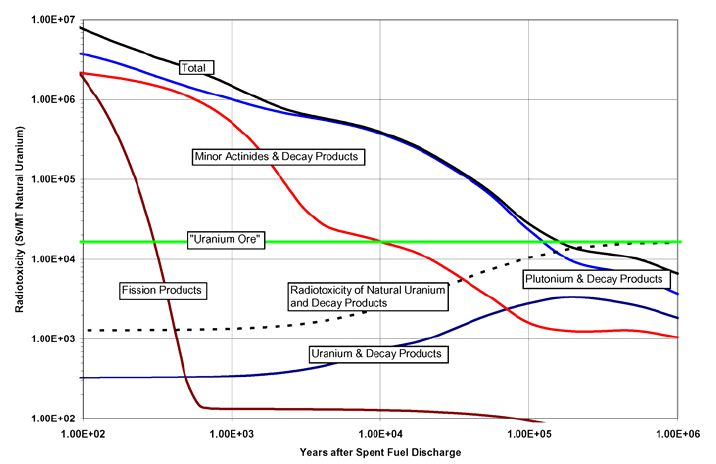
\includegraphics[width=1.0\textwidth]{./Figures/NEASpentNuclearlFuel.jpeg}
\caption{Radiotoxicity of Spent Nuclear Fuel by Component (NEA report 6090, 2006)}
\label{Fig:kinetics_spentNuclearFuelRadiotoxicity}
\end{center}
\end{figure}

The specific activity of spent nuclear fuel broken down by component is given in Fig.~\ref{Fig:kinetics_spentNuclearFuelRadiotoxicity}. Much of the long-lived radioactivity that is of major concern for the long-term disposal of spent nuclear fuel are the actinides, many of which have half-lives on the order of several thousands or a few tens of thousands of years. It is this range which is most problematic. While less radioactive than the shorter lived fission products, they are still short enough and in large enough quantities to cause a large radiation dose to anyone exposed to the material for tens of thousands of years. The plutonium isotopes and its decay products would take about 100,000 years to decay to the radioactivity level of natural uranium ore. The minor actinides are a bit shorter and require several thousands of years to similarly decay.

This length of time is much longer than human civilization and therefore plutonium and the minor actinides are the major concern with the long-term disposal of spent nuclear fuel. The fission products alone are a concern, but these \emph{only} need to be isolated for a few hundred years. While this is indeed a very long time, spanning several human lifespans, there is little question about the technical ability to engineer containers able to endure for this length of time. Indeed this provides the major motivation for recycling of spent nuclear fuel, as engineering barriers that hold for tens of thousands of years is highly questionable.

The issue of spent nuclear fuel disposal is both a technical challenge in addition to difficult raising questions of policy and environmental justice. Entire books have been written on this topic, and we will not attempt to address those questions here other than to note that radioactive wastes have a finite lifetime, as they are continually becoming less toxic overall as the natural process of radioactive decay proceeds. Other industrial wastes, produced in far greater quantities, have effectively infinite lifetimes. So while the disposal of spent nuclear fuel is an important societal problem that needs to be addressed, other than its toxicity being derived from radiation as opposed to chemistry, the questions it poses are very similar. Indeed, because of the energy density of nuclear fuels, the quantities generated are much smaller and are quite manageable.

